% Options for packages loaded elsewhere
\PassOptionsToPackage{unicode}{hyperref}
\PassOptionsToPackage{hyphens}{url}
\PassOptionsToPackage{dvipsnames,svgnames,x11names}{xcolor}
%
\documentclass[
]{book}
\usepackage{amsmath,amssymb}
\usepackage{iftex}
\ifPDFTeX
  \usepackage[T1]{fontenc}
  \usepackage[utf8]{inputenc}
  \usepackage{textcomp} % provide euro and other symbols
\else % if luatex or xetex
  \usepackage{unicode-math} % this also loads fontspec
  \defaultfontfeatures{Scale=MatchLowercase}
  \defaultfontfeatures[\rmfamily]{Ligatures=TeX,Scale=1}
\fi
\usepackage{lmodern}
\ifPDFTeX\else
  % xetex/luatex font selection
\fi
% Use upquote if available, for straight quotes in verbatim environments
\IfFileExists{upquote.sty}{\usepackage{upquote}}{}
\IfFileExists{microtype.sty}{% use microtype if available
  \usepackage[]{microtype}
  \UseMicrotypeSet[protrusion]{basicmath} % disable protrusion for tt fonts
}{}
\makeatletter
\@ifundefined{KOMAClassName}{% if non-KOMA class
  \IfFileExists{parskip.sty}{%
    \usepackage{parskip}
  }{% else
    \setlength{\parindent}{0pt}
    \setlength{\parskip}{6pt plus 2pt minus 1pt}}
}{% if KOMA class
  \KOMAoptions{parskip=half}}
\makeatother
\usepackage{xcolor}
\usepackage[b5paper,tmargin=1.5cm,bmargin=1.5cm,lmargin=1.0cm,rmargin=1.0cm]{geometry}
\usepackage{color}
\usepackage{fancyvrb}
\newcommand{\VerbBar}{|}
\newcommand{\VERB}{\Verb[commandchars=\\\{\}]}
\DefineVerbatimEnvironment{Highlighting}{Verbatim}{commandchars=\\\{\}}
% Add ',fontsize=\small' for more characters per line
\usepackage{framed}
\definecolor{shadecolor}{RGB}{248,248,248}
\newenvironment{Shaded}{\begin{snugshade}}{\end{snugshade}}
\newcommand{\AlertTok}[1]{\textcolor[rgb]{0.94,0.16,0.16}{#1}}
\newcommand{\AnnotationTok}[1]{\textcolor[rgb]{0.56,0.35,0.01}{\textbf{\textit{#1}}}}
\newcommand{\AttributeTok}[1]{\textcolor[rgb]{0.13,0.29,0.53}{#1}}
\newcommand{\BaseNTok}[1]{\textcolor[rgb]{0.00,0.00,0.81}{#1}}
\newcommand{\BuiltInTok}[1]{#1}
\newcommand{\CharTok}[1]{\textcolor[rgb]{0.31,0.60,0.02}{#1}}
\newcommand{\CommentTok}[1]{\textcolor[rgb]{0.56,0.35,0.01}{\textit{#1}}}
\newcommand{\CommentVarTok}[1]{\textcolor[rgb]{0.56,0.35,0.01}{\textbf{\textit{#1}}}}
\newcommand{\ConstantTok}[1]{\textcolor[rgb]{0.56,0.35,0.01}{#1}}
\newcommand{\ControlFlowTok}[1]{\textcolor[rgb]{0.13,0.29,0.53}{\textbf{#1}}}
\newcommand{\DataTypeTok}[1]{\textcolor[rgb]{0.13,0.29,0.53}{#1}}
\newcommand{\DecValTok}[1]{\textcolor[rgb]{0.00,0.00,0.81}{#1}}
\newcommand{\DocumentationTok}[1]{\textcolor[rgb]{0.56,0.35,0.01}{\textbf{\textit{#1}}}}
\newcommand{\ErrorTok}[1]{\textcolor[rgb]{0.64,0.00,0.00}{\textbf{#1}}}
\newcommand{\ExtensionTok}[1]{#1}
\newcommand{\FloatTok}[1]{\textcolor[rgb]{0.00,0.00,0.81}{#1}}
\newcommand{\FunctionTok}[1]{\textcolor[rgb]{0.13,0.29,0.53}{\textbf{#1}}}
\newcommand{\ImportTok}[1]{#1}
\newcommand{\InformationTok}[1]{\textcolor[rgb]{0.56,0.35,0.01}{\textbf{\textit{#1}}}}
\newcommand{\KeywordTok}[1]{\textcolor[rgb]{0.13,0.29,0.53}{\textbf{#1}}}
\newcommand{\NormalTok}[1]{#1}
\newcommand{\OperatorTok}[1]{\textcolor[rgb]{0.81,0.36,0.00}{\textbf{#1}}}
\newcommand{\OtherTok}[1]{\textcolor[rgb]{0.56,0.35,0.01}{#1}}
\newcommand{\PreprocessorTok}[1]{\textcolor[rgb]{0.56,0.35,0.01}{\textit{#1}}}
\newcommand{\RegionMarkerTok}[1]{#1}
\newcommand{\SpecialCharTok}[1]{\textcolor[rgb]{0.81,0.36,0.00}{\textbf{#1}}}
\newcommand{\SpecialStringTok}[1]{\textcolor[rgb]{0.31,0.60,0.02}{#1}}
\newcommand{\StringTok}[1]{\textcolor[rgb]{0.31,0.60,0.02}{#1}}
\newcommand{\VariableTok}[1]{\textcolor[rgb]{0.00,0.00,0.00}{#1}}
\newcommand{\VerbatimStringTok}[1]{\textcolor[rgb]{0.31,0.60,0.02}{#1}}
\newcommand{\WarningTok}[1]{\textcolor[rgb]{0.56,0.35,0.01}{\textbf{\textit{#1}}}}
\usepackage{longtable,booktabs,array}
\usepackage{calc} % for calculating minipage widths
% Correct order of tables after \paragraph or \subparagraph
\usepackage{etoolbox}
\makeatletter
\patchcmd\longtable{\par}{\if@noskipsec\mbox{}\fi\par}{}{}
\makeatother
% Allow footnotes in longtable head/foot
\IfFileExists{footnotehyper.sty}{\usepackage{footnotehyper}}{\usepackage{footnote}}
\makesavenoteenv{longtable}
\usepackage{graphicx}
\makeatletter
\def\maxwidth{\ifdim\Gin@nat@width>\linewidth\linewidth\else\Gin@nat@width\fi}
\def\maxheight{\ifdim\Gin@nat@height>\textheight\textheight\else\Gin@nat@height\fi}
\makeatother
% Scale images if necessary, so that they will not overflow the page
% margins by default, and it is still possible to overwrite the defaults
% using explicit options in \includegraphics[width, height, ...]{}
\setkeys{Gin}{width=\maxwidth,height=\maxheight,keepaspectratio}
% Set default figure placement to htbp
\makeatletter
\def\fps@figure{htbp}
\makeatother
\setlength{\emergencystretch}{3em} % prevent overfull lines
\providecommand{\tightlist}{%
  \setlength{\itemsep}{0pt}\setlength{\parskip}{0pt}}
\setcounter{secnumdepth}{5}
\newlength{\cslhangindent}
\setlength{\cslhangindent}{1.5em}
\newlength{\csllabelwidth}
\setlength{\csllabelwidth}{3em}
\newlength{\cslentryspacingunit} % times entry-spacing
\setlength{\cslentryspacingunit}{\parskip}
\newenvironment{CSLReferences}[2] % #1 hanging-ident, #2 entry spacing
 {% don't indent paragraphs
  \setlength{\parindent}{0pt}
  % turn on hanging indent if param 1 is 1
  \ifodd #1
  \let\oldpar\par
  \def\par{\hangindent=\cslhangindent\oldpar}
  \fi
  % set entry spacing
  \setlength{\parskip}{#2\cslentryspacingunit}
 }%
 {}
\usepackage{calc}
\newcommand{\CSLBlock}[1]{#1\hfill\break}
\newcommand{\CSLLeftMargin}[1]{\parbox[t]{\csllabelwidth}{#1}}
\newcommand{\CSLRightInline}[1]{\parbox[t]{\linewidth - \csllabelwidth}{#1}\break}
\newcommand{\CSLIndent}[1]{\hspace{\cslhangindent}#1}
\usepackage{booktabs}
% \usepackage{fontspec} %這個可能原本文檔就已經有了,放入時候check一下
% \usepackage{CJKutf8}
% \usepackage[UTF8]{inputenc}
\usepackage{CJK}
% \usepackage{xeCJK}

%英文字體調整(有時候交中文文件可能有規定對應的英文字體)
% \setmainfont{Times New Roman}
% \setmainfont{Noto Sans}

%中文字體main跟mono都需要哦,最後面的SC是簡體中文,也可以改成TC,不過SC的破字會比較少
% \setCJKmainfont{NotoSansTC-Regular.otf}
% \setCJKmonofont{NotoSansTC-Regular.otf}

% \usepackage{bm}
\usepackage{amsmath,amssymb}
% \usepackage[pagebackref=true]{hyperref}
% \usepackage[backref]{hyperref}
\usepackage[]{hyperref}
\usepackage[hyperpageref]{backref}
\hypersetup{
    colorlinks=true,
    linkcolor=blue,
    filecolor=magenta,      
    urlcolor=cyan
}

% \usepackage{fdsymbol} % vector over accent, but will use mathptmx
%% replace the rather ugly mathptmx \sum operator with the equivalent Computer Modern one
% \let\sum\relax
% \DeclareSymbolFont{CMlargesymbols}{OMX}{cmex}{m}{n}
% \DeclareMathSymbol{\sum}{\mathop}{CMlargesymbols}{"50}

\usepackage{cancel} % demo usepackage in PDF and require in HTML

% to wrap the text inside the margins of the PDF document when using code chunks in bookdown
\usepackage{fvextra}
\DefineVerbatimEnvironment{Highlighting}{Verbatim}{breaklines,commandchars=\\\{\}}

% \usepackage[backend=bibtex]{biblatex}
% \usepackage[backend=biber]{biblatex}
% \usepackage[]{biblatex}
% \DeclarePrintbibliographyDefaults{heading=bibintoc}

% \let\oldpb\printbibliography
% \renewcommand{\printbibliography}{\oldpb[heading=bibintoc]}

% SVG
\usepackage{svg}

% TikZ
\usepackage{tikz}
\usepackage{tikz-3dplot}
\usepackage{pgfplots}
\pgfplotsset{compat=1.15}
% animation
\usepackage[autoplay]{animate}

% xcolor colorbox
% https://www.overleaf.com/learn/latex/Using_colors_in_LaTeX
\usepackage[dvipsnames]{xcolor}
% \usepackage[svgnames]{xcolor}
% \usepackage[x11names]{xcolor}

\usepackage{mathrsfs}
\usetikzlibrary{arrows}
% \pagestyle{empty}
% \newcommand{\degre}{\ensuremath{^\circ}}

\usepackage[all]{xy}

% LaTeX Error: Too deeply nested
% https://stackoverflow.com/questions/57945414/too-deeply-nested-at-just-fourth-nesting-level-using-pandoc-with-markdown
\usepackage{enumitem}
\setlistdepth{20}
\renewlist{itemize}{itemize}{20}
\renewlist{enumerate}{enumerate}{20}
\setlist[itemize]{label=$\cdot$}
\setlist[itemize,1]{label=\textbullet}
\setlist[itemize,2]{label=--}
\setlist[itemize,3]{label=*}

% multicolumn
% https://bookdown.org/yihui/rmarkdown-cookbook/multi-column.html
\newenvironment{cols}[1][]{}{}

\newenvironment{col}[1]{\begin{minipage}{#1}\ignorespaces}{%
\end{minipage}
\ifhmode\unskip\fi
\aftergroup\useignorespacesandallpars}

\def\useignorespacesandallpars#1\ignorespaces\fi{%
#1\fi\ignorespacesandallpars}

\makeatletter
\def\ignorespacesandallpars{%
  \@ifnextchar\par
    {\expandafter\ignorespacesandallpars\@gobble}%
    {}%
}
\makeatother
\ifLuaTeX
  \usepackage{selnolig}  % disable illegal ligatures
\fi
\IfFileExists{bookmark.sty}{\usepackage{bookmark}}{\usepackage{hyperref}}
\IfFileExists{xurl.sty}{\usepackage{xurl}}{} % add URL line breaks if available
\urlstyle{same}
\hypersetup{
  pdftitle={math},
  pdfauthor={Joey Yu Hsu},
  colorlinks=true,
  linkcolor={Maroon},
  filecolor={Maroon},
  citecolor={Blue},
  urlcolor={Blue},
  pdfcreator={LaTeX via pandoc}}

\title{math}
\author{Joey Yu Hsu}
\date{2024-03-02}

\usepackage{amsthm}
\newtheorem{theorem}{Theorem}[chapter]
\newtheorem{lemma}{Lemma}[chapter]
\newtheorem{corollary}{Corollary}[chapter]
\newtheorem{proposition}{Proposition}[chapter]
\newtheorem{conjecture}{Conjecture}[chapter]
\theoremstyle{definition}
\newtheorem{definition}{Definition}[chapter]
\theoremstyle{definition}
\newtheorem{example}{Example}[chapter]
\theoremstyle{definition}
\newtheorem{exercise}{Exercise}[chapter]
\theoremstyle{definition}
\newtheorem{hypothesis}{Hypothesis}[chapter]
\theoremstyle{remark}
\newtheorem*{remark}{Remark}
\newtheorem*{solution}{Solution}
\begin{document}
\maketitle

{
\hypersetup{linkcolor=}
\setcounter{tocdepth}{1}
\tableofcontents
}
\hypertarget{index}{%
\chapter*{index}\label{index}}
\addcontentsline{toc}{chapter}{index}

math on bookdown started on 2024/01/28

\hypertarget{part-by-descipline}{%
\part{by descipline}\label{part-by-descipline}}

\hypertarget{nice-label}{%
\chapter{mathematics}\label{nice-label}}

\begin{itemize}
\tightlist
\item
  formula typesetting

  \begin{itemize}
  \tightlist
  \item
    TeX

    \begin{itemize}
    \tightlist
    \item
      LaTeX

      \begin{itemize}
      \tightlist
      \item
        pdfLaTeX
      \item
        XeLaTeX
      \item
        editor/tool:

        \begin{itemize}
        \tightlist
        \item
          LyX
        \item
          OverLeaf
        \item
          MathPix Snip
        \item
          Micro\$oft Office Word

          \begin{itemize}
          \tightlist
          \item
            WordTeX \url{https://tomwildenhain.com/wordtex/}

            \begin{itemize}
            \tightlist
            \item
              Pandoc dependent
            \end{itemize}
          \item
            \url{https://superuser.com/questions/1114697/select-a-different-math-font-in-microsoft-word}
          \item
            \url{https://www.youtube.com/watch?v=jlX_pThh7z8}
          \end{itemize}
        \item
          Micro\$oft Office PowerPoint

          \begin{itemize}
          \tightlist
          \item
            IguanaTeX \url{https://www.jonathanleroux.org/software/iguanatex/}
          \end{itemize}
        \end{itemize}
      \end{itemize}
    \end{itemize}
  \item
    MathML
  \item
    MathJax: JavaScript
  \end{itemize}
\item
  symbolic computing

  \begin{itemize}
  \tightlist
  \item
    Maple: by MapleSoft
  \item
    Mathematica: by Wolfram
  \end{itemize}
\item
  numeric computing

  \begin{itemize}
  \tightlist
  \item
    MatLab: by MathWorks
  \end{itemize}
\end{itemize}

\protect\hyperlink{equivalence-relation}{equivalence relation}\textsuperscript{{[}\ref{equivalence-relation}{]}}

\protect\hyperlink{equivalence-class}{equivalence class}\textsuperscript{{[}\ref{equivalence-class}{]}}

\protect\hyperlink{partition}{partition}\textsuperscript{{[}\ref{partition}{]}}

\hypertarget{physics}{%
\chapter{physics}\label{physics}}

\begin{itemize}
\tightlist
\item
  relativity

  \begin{itemize}
  \tightlist
  \item
    special relativity

    \begin{itemize}
    \tightlist
    \item
      \protect\hyperlink{lorentz-transformation}{Lorentz transformation}\textsuperscript{{[}\ref{lorentz-transformation}{]}}
    \end{itemize}
  \item
    general relativity
  \end{itemize}
\item
  analytic mechanics

  \begin{itemize}
  \tightlist
  \item
    {[}Lagrangian mechanics{]}
  \item
    Hamiltonian mechanics
  \end{itemize}
\item
  electromagnetism
\item
  quantum mechanics
\item
  field theory
\end{itemize}

\hypertarget{plot}{%
\chapter{plot}\label{plot}}

\begin{itemize}
\tightlist
\item
  LaTeX

  \begin{itemize}
  \tightlist
  \item
    \protect\hyperlink{tikz}{TikZ}\textsuperscript{{[}\ref{tikz}{]}}

    \begin{itemize}
    \tightlist
    \item
      TikZ-3Dplot
    \item
      PGFplots
    \end{itemize}
  \item
    xypic = \protect\hyperlink{xy-pic}{xy-pic}\textsuperscript{{[}\ref{xy-pic}{]}}
  \end{itemize}
\item
  \href{https://www.overleaf.com/}{OverLeaf}
\item
  \href{https://www.mathcha.io/}{MathCha}
\item
  \href{https://www.geogebra.org/}{GeoGebra}

  \begin{itemize}
  \tightlist
  \item
    \href{https://www.geogebra.org/classic}{GeoGebra Classic}: to export TikZ
  \item
    \href{https://www.geogebra.org/calculator}{GeoGebra Calculator Suite}
  \end{itemize}
\item
  Python

  \begin{itemize}
  \tightlist
  \item
    MatPlotLib
  \item
    Seaborn
  \item
    Plotly
  \item
    Manim
  \end{itemize}
\end{itemize}

neural network plot/draw
\url{https://github.com/ashishpatel26/Tools-to-Design-or-Visualize-Architecture-of-Neural-Network}

\hypertarget{programming-language}{%
\chapter{programming language}\label{programming-language}}

\begin{itemize}
\tightlist
\item
  \protect\hyperlink{python}{Python}\textsuperscript{{[}\ref{python}{]}}
\item
  JavaScript
\item
  SQL = structured query language
\item
  \protect\hyperlink{r}{R}\textsuperscript{{[}\ref{r}{]}}

  \begin{itemize}
  \tightlist
  \item
    RMarkdown

    \begin{itemize}
    \tightlist
    \item
      Bookdown
    \end{itemize}
  \item
    knitr: engine

    \begin{itemize}
    \tightlist
    \item
      TikZ
    \end{itemize}
  \item
    reticulate: Python
  \end{itemize}
\item
  C\#

  \begin{itemize}
  \tightlist
  \item
    web

    \begin{itemize}
    \tightlist
    \item
      MVC
    \item
      .NET
    \end{itemize}
  \item
    desktop

    \begin{itemize}
    \tightlist
    \item
      UWP = Universal Windows Platform
    \item
      WPF = Windows Presentation Foundation
    \item
      WinForms = Windows Forms
    \end{itemize}
  \item
    3D/game

    \begin{itemize}
    \tightlist
    \item
      Unity
    \end{itemize}
  \end{itemize}
\end{itemize}

\hypertarget{machine-learning}{%
\chapter{machine learning}\label{machine-learning}}

\hypertarget{part-by-date}{%
\part{by date}\label{part-by-date}}

\hypertarget{a-minimal-book-example}{%
\chapter{A Minimal Book Example}\label{a-minimal-book-example}}

\hypertarget{about}{%
\section{About}\label{about}}

This is a \emph{sample} book written in \textbf{Markdown}. You can use anything that Pandoc's Markdown supports; for example, a math equation \(a^2 + b^2 = c^2\).

\hypertarget{usage}{%
\subsection{Usage}\label{usage}}

Each \textbf{bookdown} chapter is an .Rmd file, and each .Rmd file can contain one (and only one) chapter. A chapter \emph{must} start with a first-level heading: \texttt{\#\ A\ good\ chapter}, and can contain one (and only one) first-level heading.

Use second-level and higher headings within chapters like: \texttt{\#\#\ A\ short\ section} or \texttt{\#\#\#\ An\ even\ shorter\ section}.

The \texttt{index.Rmd} file is required, and is also your first book chapter. It will be the homepage when you render the book.

\hypertarget{render-book}{%
\subsection{Render book}\label{render-book}}

You can render the HTML version of this example book without changing anything:

\begin{enumerate}
\def\labelenumi{\arabic{enumi}.}
\item
  Find the \textbf{Build} pane in the RStudio IDE, and
\item
  Click on \textbf{Build Book}, then select your output format, or select ``All formats'' if you'd like to use multiple formats from the same book source files.
\end{enumerate}

Or build the book from the R console:

\begin{Shaded}
\begin{Highlighting}[]
\NormalTok{bookdown}\SpecialCharTok{::}\FunctionTok{render\_book}\NormalTok{()}
\end{Highlighting}
\end{Shaded}

To render this example to PDF as a \texttt{bookdown::pdf\_book}, you'll need to install XeLaTeX. You are recommended to install TinyTeX (which includes XeLaTeX): \url{https://yihui.org/tinytex/}.

\hypertarget{preview-book}{%
\subsection{Preview book}\label{preview-book}}

As you work, you may start a local server to live preview this HTML book. This preview will update as you edit the book when you save individual .Rmd files. You can start the server in a work session by using the RStudio add-in ``Preview book'', or from the R console:

\begin{Shaded}
\begin{Highlighting}[]
\NormalTok{bookdown}\SpecialCharTok{::}\FunctionTok{serve\_book}\NormalTok{()}
\end{Highlighting}
\end{Shaded}

\hypertarget{hello-bookdown}{%
\section{Hello bookdown}\label{hello-bookdown}}

All chapters start with a first-level heading followed by your chapter title, like the line above. There should be only one first-level heading (\texttt{\#}) per .Rmd file.

\hypertarget{a-section}{%
\subsection{A section}\label{a-section}}

All chapter sections start with a second-level (\texttt{\#\#}) or higher heading followed by your section title, like the sections above and below here. You can have as many as you want within a chapter.

\hypertarget{an-unnumbered-section}{%
\subsubsection*{An unnumbered section}\label{an-unnumbered-section}}
\addcontentsline{toc}{subsubsection}{An unnumbered section}

Chapters and sections are numbered by default. To un-number a heading, add a \texttt{\{.unnumbered\}} or the shorter \texttt{\{-\}} at the end of the heading, like in this section.

\hypertarget{cross}{%
\section{Cross-references}\label{cross}}

Cross-references make it easier for your readers to find and link to elements in your book.

\hypertarget{chapters-and-sub-chapters}{%
\subsection{Chapters and sub-chapters}\label{chapters-and-sub-chapters}}

There are two steps to cross-reference any heading:

\begin{enumerate}
\def\labelenumi{\arabic{enumi}.}
\tightlist
\item
  Label the heading: \texttt{\#\ Hello\ world\ \{\#nice-label\}}.

  \begin{itemize}
  \tightlist
  \item
    Leave the label off if you like the automated heading generated based on your heading title: for example, \texttt{\#\ Hello\ world} = \texttt{\#\ Hello\ world\ \{\#hello-world\}}.
  \item
    To label an un-numbered heading, use: \texttt{\#\ Hello\ world\ \{-\#nice-label\}} or \texttt{\{\#\ Hello\ world\ .unnumbered\}}.
  \end{itemize}
\item
  Next, reference the labeled heading anywhere in the text using \texttt{\textbackslash{}@ref(nice-label)}; for example, please see Chapter \ref{cross}.

  \begin{itemize}
  \tightlist
  \item
    If you prefer text as the link instead of a numbered reference use: \protect\hyperlink{cross}{any text you want can go here}.
  \end{itemize}
\end{enumerate}

\hypertarget{captioned-figures-and-tables}{%
\subsection{Captioned figures and tables}\label{captioned-figures-and-tables}}

Figures and tables \emph{with captions} can also be cross-referenced from elsewhere in your book using \texttt{\textbackslash{}@ref(fig:chunk-label)} and \texttt{\textbackslash{}@ref(tab:chunk-label)}, respectively.

See Figure \ref{fig:nice-fig}.

\begin{Shaded}
\begin{Highlighting}[]
\FunctionTok{par}\NormalTok{(}\AttributeTok{mar =} \FunctionTok{c}\NormalTok{(}\DecValTok{4}\NormalTok{, }\DecValTok{4}\NormalTok{, .}\DecValTok{1}\NormalTok{, .}\DecValTok{1}\NormalTok{))}
\FunctionTok{plot}\NormalTok{(pressure, }\AttributeTok{type =} \StringTok{\textquotesingle{}b\textquotesingle{}}\NormalTok{, }\AttributeTok{pch =} \DecValTok{19}\NormalTok{)}
\end{Highlighting}
\end{Shaded}

\begin{figure}

{\centering 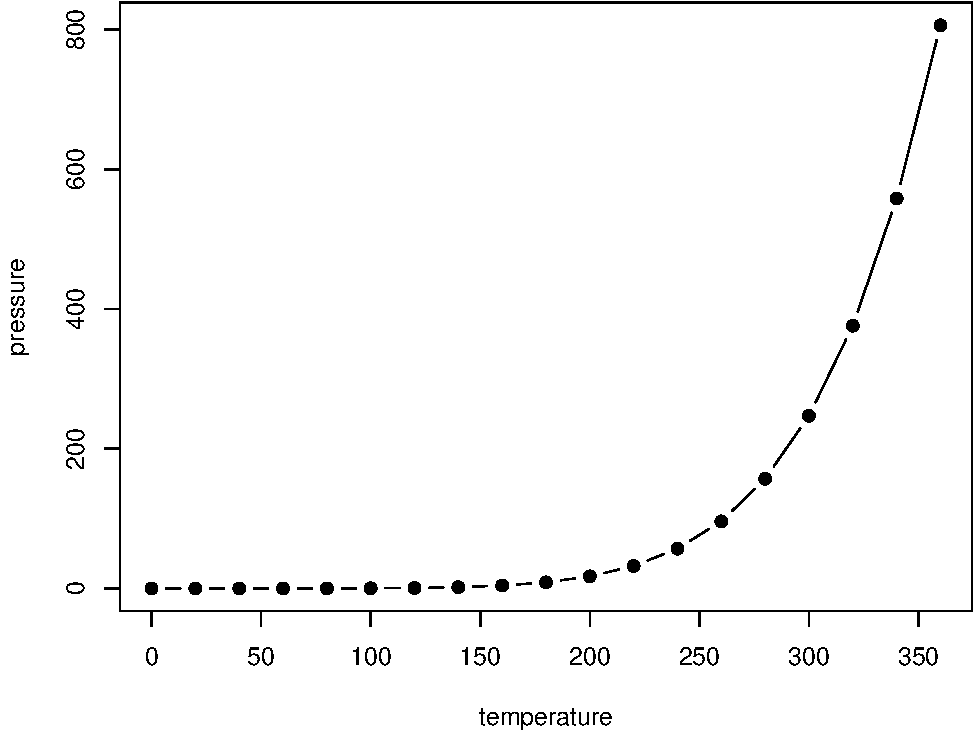
\includegraphics[width=0.8\linewidth]{202401280000-minimal-book-example_files/figure-latex/nice-fig-1} 

}

\caption{Here is a nice figure!}\label{fig:nice-fig}
\end{figure}

Don't miss Table \ref{tab:nice-tab}.

\begin{Shaded}
\begin{Highlighting}[]
\NormalTok{knitr}\SpecialCharTok{::}\FunctionTok{kable}\NormalTok{(}
  \FunctionTok{head}\NormalTok{(pressure, }\DecValTok{10}\NormalTok{), }\AttributeTok{caption =} \StringTok{\textquotesingle{}Here is a nice table!\textquotesingle{}}\NormalTok{,}
  \AttributeTok{booktabs =} \ConstantTok{TRUE}
\NormalTok{)}
\end{Highlighting}
\end{Shaded}

\begin{table}

\caption{\label{tab:nice-tab}Here is a nice table!}
\centering
\begin{tabular}[t]{rr}
\toprule
temperature & pressure\\
\midrule
0 & 0.0002\\
20 & 0.0012\\
40 & 0.0060\\
60 & 0.0300\\
80 & 0.0900\\
\addlinespace
100 & 0.2700\\
120 & 0.7500\\
140 & 1.8500\\
160 & 4.2000\\
180 & 8.8000\\
\bottomrule
\end{tabular}
\end{table}

\hypertarget{parts}{%
\section{Parts}\label{parts}}

You can add parts to organize one or more book chapters together. Parts can be inserted at the top of an .Rmd file, before the first-level chapter heading in that same file.

Add a numbered part: \texttt{\#\ (PART)\ Act\ one\ \{-\}} (followed by \texttt{\#\ A\ chapter})

Add an unnumbered part: \texttt{\#\ (PART\textbackslash{}*)\ Act\ one\ \{-\}} (followed by \texttt{\#\ A\ chapter})

Add an appendix as a special kind of un-numbered part: \texttt{\#\ (APPENDIX)\ Other\ stuff\ \{-\}} (followed by \texttt{\#\ A\ chapter}). Chapters in an appendix are prepended with letters instead of numbers.

\hypertarget{footnotes-and-citations}{%
\section{Footnotes and citations}\label{footnotes-and-citations}}

\hypertarget{footnotes}{%
\subsection{Footnotes}\label{footnotes}}

Footnotes are put inside the square brackets after a caret \texttt{\^{}{[}{]}}. Like this one \footnote{This is a footnote.}.

\hypertarget{citations}{%
\subsection{Citations}\label{citations}}

Reference items in your bibliography file(s) using \texttt{@key}.

For example, we are using the \textbf{bookdown} package\textsuperscript{\protect\hyperlink{ref-R-bookdown}{1}} (check out the last code chunk in index.Rmd to see how this citation key was added) in this sample book, which was built on top of R Markdown and \textbf{knitr}\textsuperscript{\protect\hyperlink{ref-xie2015}{2}} (this citation was added manually in an external file book.bib).
Note that the \texttt{.bib} files need to be listed in the index.Rmd with the YAML \texttt{bibliography} key.

The RStudio Visual Markdown Editor can also make it easier to insert citations: \url{https://rstudio.github.io/visual-markdown-editing/\#/citations}

\hypertarget{blocks}{%
\section{Blocks}\label{blocks}}

\hypertarget{equations}{%
\subsection{Equations}\label{equations}}

Here is an equation.

\begin{equation} 
  f\left(k\right) = \binom{n}{k} p^k\left(1-p\right)^{n-k}
  \label{eq:binom}
\end{equation}

You may refer to using \texttt{\textbackslash{}@ref(eq:binom)}, like see Equation \eqref{eq:binom}.

\hypertarget{theorems-and-proofs}{%
\subsection{Theorems and proofs}\label{theorems-and-proofs}}

Labeled theorems can be referenced in text using \texttt{\textbackslash{}@ref(thm:tri)}, for example, check out this smart theorem \ref{thm:tri}.

\begin{theorem}
\protect\hypertarget{thm:tri}{}\label{thm:tri}For a right triangle, if \(c\) denotes the \emph{length} of the hypotenuse
and \(a\) and \(b\) denote the lengths of the \textbf{other} two sides, we have
\[a^2 + b^2 = c^2\]
\end{theorem}

Read more here \url{https://bookdown.org/yihui/bookdown/markdown-extensions-by-bookdown.html}.

\hypertarget{callout-blocks}{%
\subsection{Callout blocks}\label{callout-blocks}}

The R Markdown Cookbook provides more help on how to use custom blocks to design your own callouts: \url{https://bookdown.org/yihui/rmarkdown-cookbook/custom-blocks.html}

\hypertarget{sharing-your-book}{%
\section{Sharing your book}\label{sharing-your-book}}

\hypertarget{publishing}{%
\subsection{Publishing}\label{publishing}}

HTML books can be published online, see: \url{https://bookdown.org/yihui/bookdown/publishing.html}

\hypertarget{pages}{%
\subsection{404 pages}\label{pages}}

By default, users will be directed to a 404 page if they try to access a webpage that cannot be found. If you'd like to customize your 404 page instead of using the default, you may add either a \texttt{\_404.Rmd} or \texttt{\_404.md} file to your project root and use code and/or Markdown syntax.

\hypertarget{metadata-for-sharing}{%
\subsection{Metadata for sharing}\label{metadata-for-sharing}}

Bookdown HTML books will provide HTML metadata for social sharing on platforms like Twitter, Facebook, and LinkedIn, using information you provide in the \texttt{index.Rmd} YAML. To setup, set the \texttt{url} for your book and the path to your \texttt{cover-image} file. Your book's \texttt{title} and \texttt{description} are also used.

This \texttt{gitbook} uses the same social sharing data across all chapters in your book- all links shared will look the same.

Specify your book's source repository on GitHub using the \texttt{edit} key under the configuration options in the \texttt{\_output.yml} file, which allows users to suggest an edit by linking to a chapter's source file.

Read more about the features of this output format here:

\url{https://pkgs.rstudio.com/bookdown/reference/gitbook.html}

Or use:

\begin{Shaded}
\begin{Highlighting}[]
\NormalTok{?bookdown}\SpecialCharTok{::}\NormalTok{gitbook}
\end{Highlighting}
\end{Shaded}

\hypertarget{test}{%
\chapter{test}\label{test}}

\url{https://bookdown.org/yihui/rmarkdown-cookbook/verbatim-code-chunks.html}

\hypertarget{rstudio}{%
\section{RStudio}\label{rstudio}}

\hypertarget{rtools}{%
\subsection{Rtools}\label{rtools}}

Rtools43 for Windows
\url{https://cran.r-project.org/bin/windows/Rtools/rtools43/rtools.html}

\hypertarget{addins}{%
\subsection{addins}\label{addins}}

\url{https://github.com/rstudio/addinexamples}

\begin{verbatim}
if (!requireNamespace("devtools", quietly = TRUE))
  install.packages("devtools")
  
devtools::install_github("rstudio/htmltools")
devtools::install_github("rstudio/shiny")
devtools::install_github("rstudio/miniUI")
\end{verbatim}

\hypertarget{rmarkdown}{%
\section{RMarkdown}\label{rmarkdown}}

\url{https://www.rstudio.com/wp-content/uploads/2015/02/rmarkdown-cheatsheet.pdf}

\url{https://slides.yihui.org/2020-taipei-satrday-rmarkdown.html\#1}

\hypertarget{url}{%
\subsection{URL}\label{url}}

\url{https://stackoverflow.com/questions/29787850/how-do-i-add-a-url-to-r-markdown}

\hypertarget{superscript-and-subscript}{%
\subsection{superscript and subscript}\label{superscript-and-subscript}}

script\textsuperscript{superscript}\textsubscript{subscript}

\begin{Shaded}
\begin{Highlighting}[]
\NormalTok{script\^{}superscript\^{}}
\end{Highlighting}
\end{Shaded}

script\textsuperscript{superscript}

\begin{Shaded}
\begin{Highlighting}[]
\NormalTok{\textasciitilde{}subscript\textasciitilde{}}
\end{Highlighting}
\end{Shaded}

script\textsubscript{subscript}

\hypertarget{latex}{%
\subsubsection{LaTeX}\label{latex}}

\url{https://tex.stackexchange.com/questions/580824/subscript-not-distinguished-enough}

\url{https://tex.stackexchange.com/questions/262295/make-subscript-size-smaller-always}

\hypertarget{equation}{%
\subsection{equation}\label{equation}}

\url{https://stackoverflow.com/questions/26049762/erroneous-nesting-of-equation-structures-in-using-beginalign-in-a-multi-l}

\hypertarget{image}{%
\subsection{image}\label{image}}

\url{https://stackoverflow.com/questions/25166624/insert-picture-table-in-r-markdown}

\begin{figure}
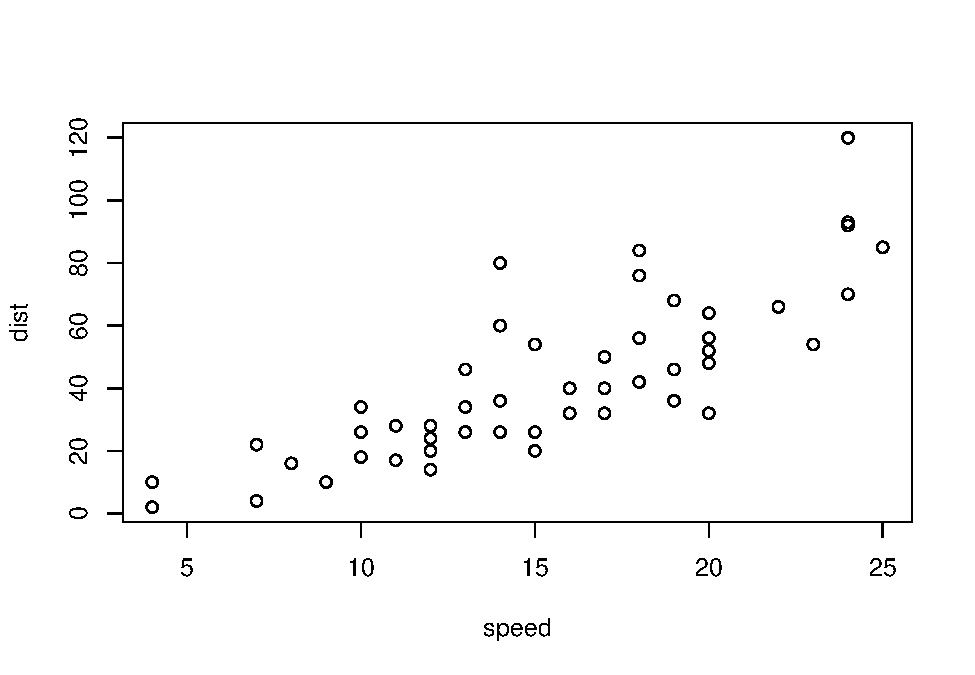
\includegraphics[width=0.75\linewidth]{202401280001-test_files/figure-latex/unnamed-chunk-4-1} \caption{conic sections}\label{fig:unnamed-chunk-4}
\end{figure}

\hypertarget{svg}{%
\subsubsection{SVG}\label{svg}}

\url{https://stackoverflow.com/questions/50165404/how-to-make-a-pdf-using-bookdown-including-svg-images}

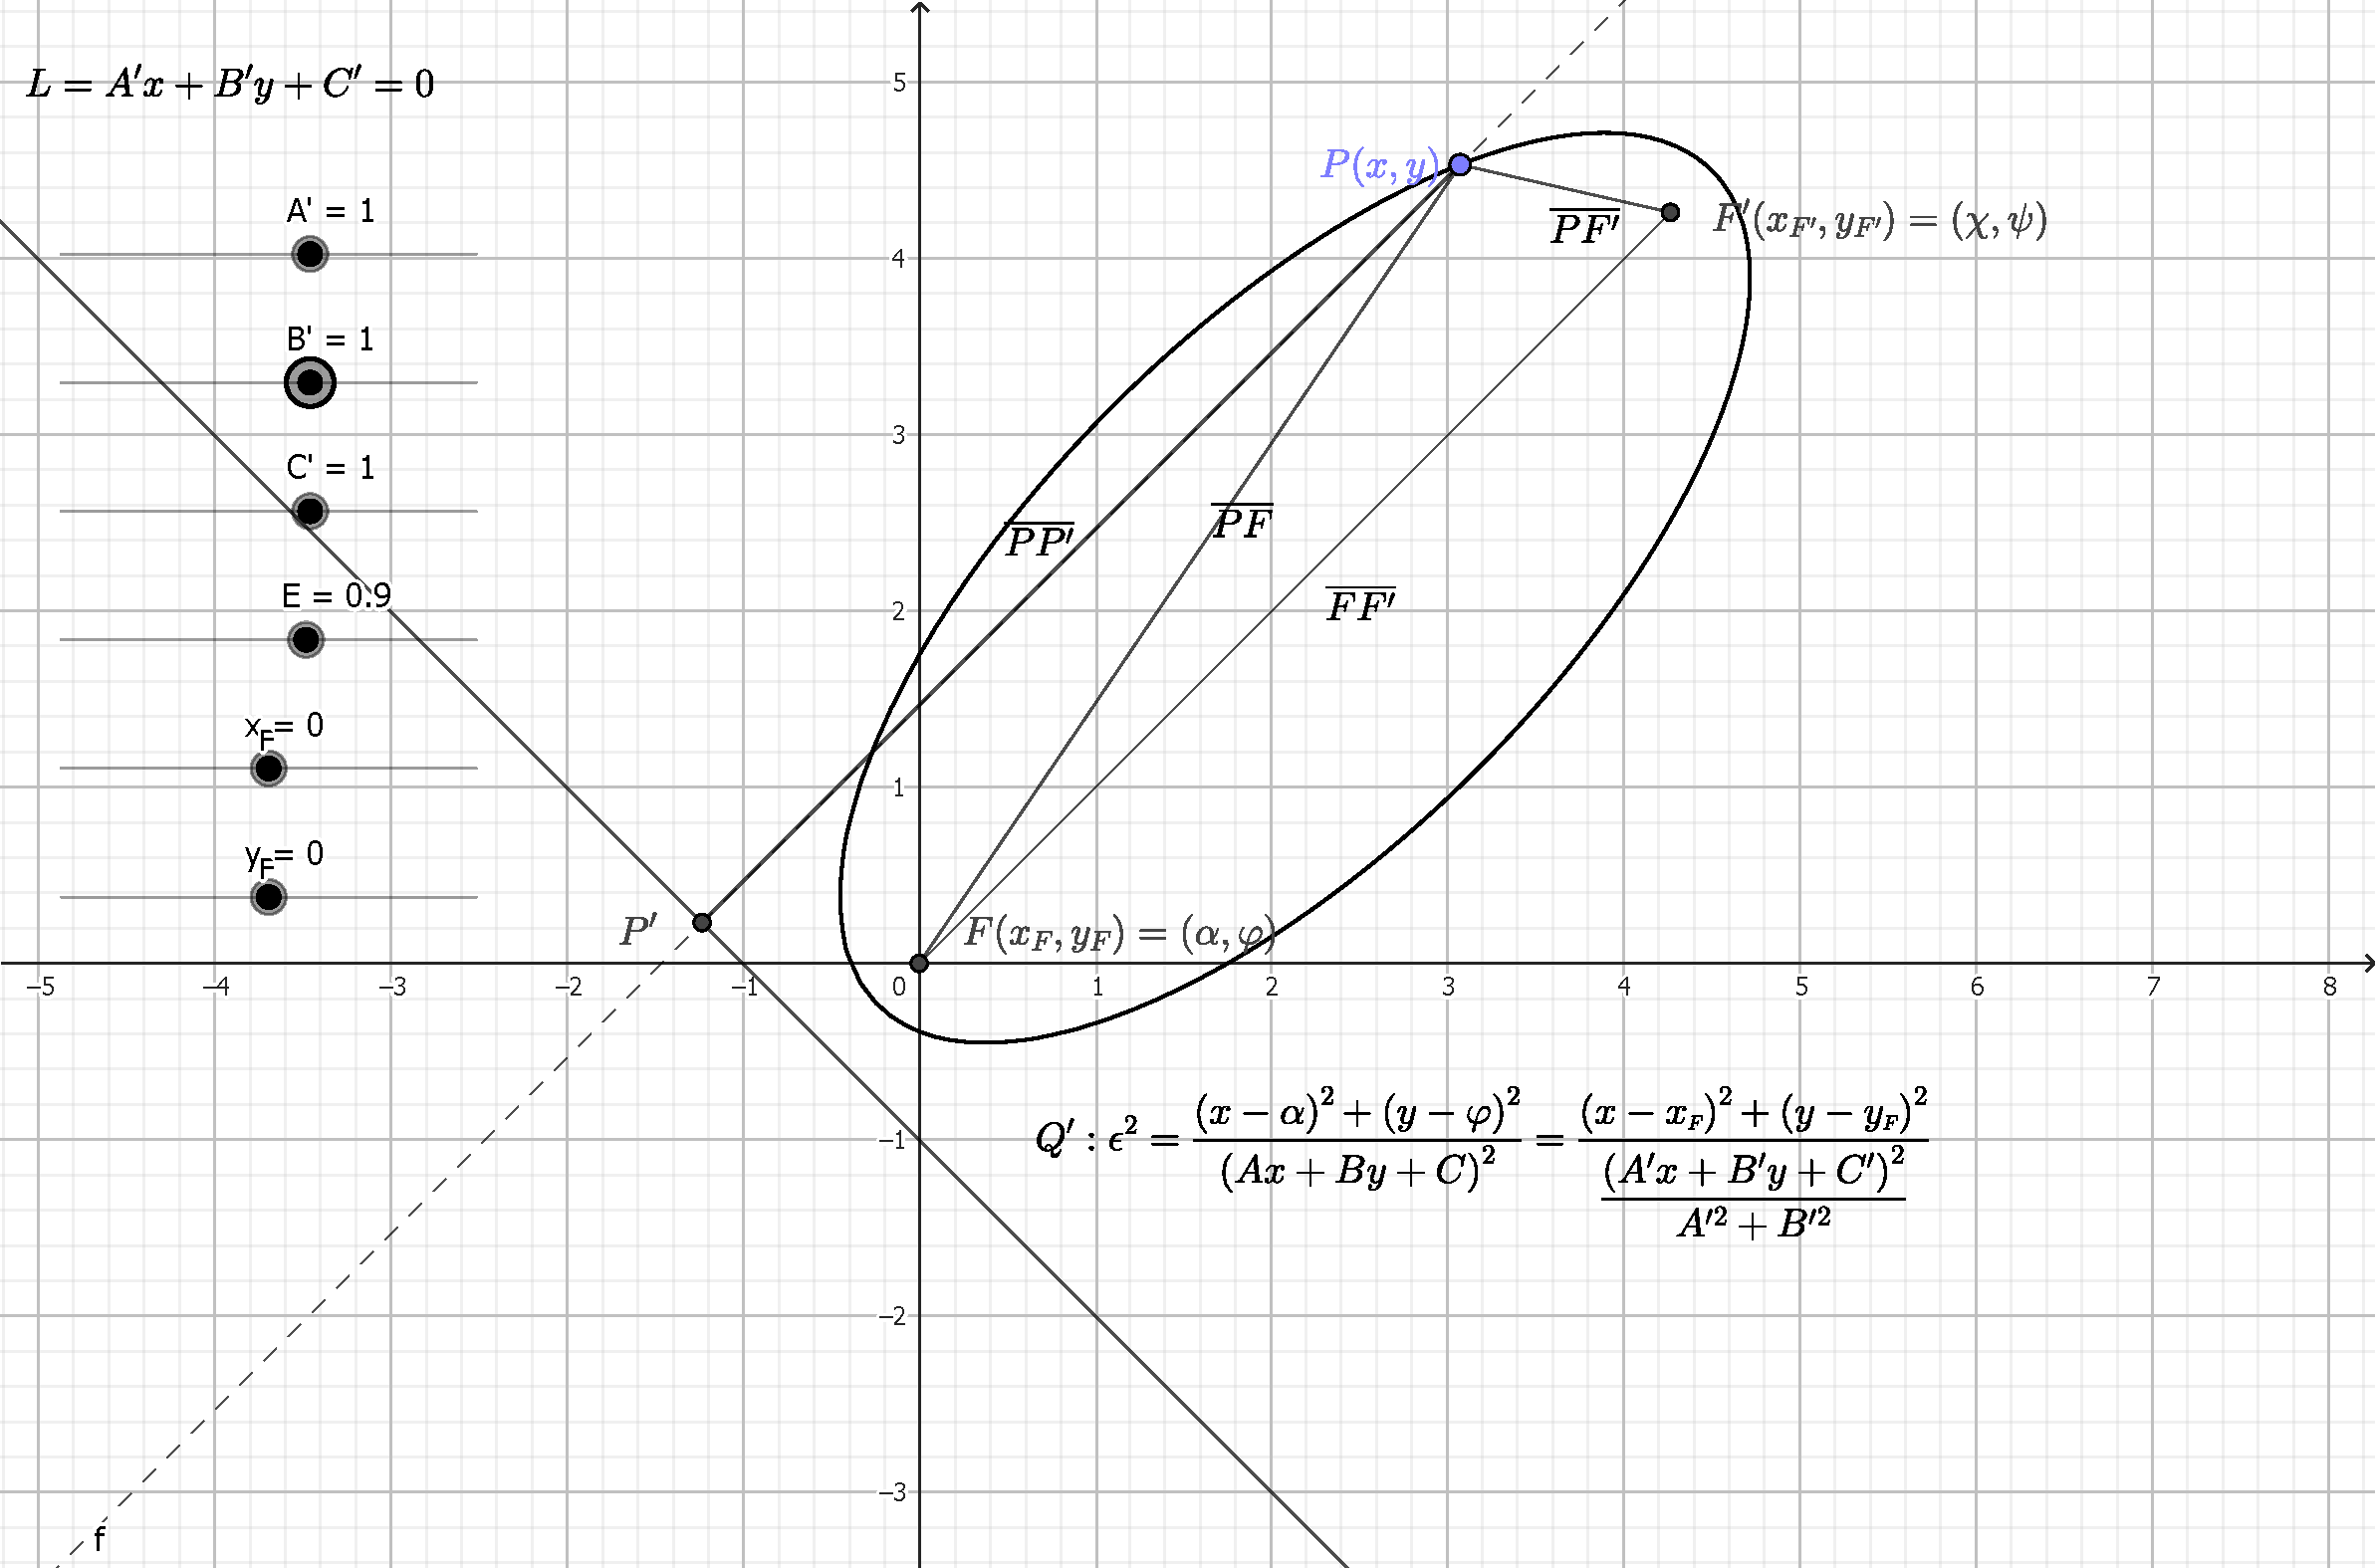
\includegraphics{img/conic-sections.pdf}

\begin{figure}
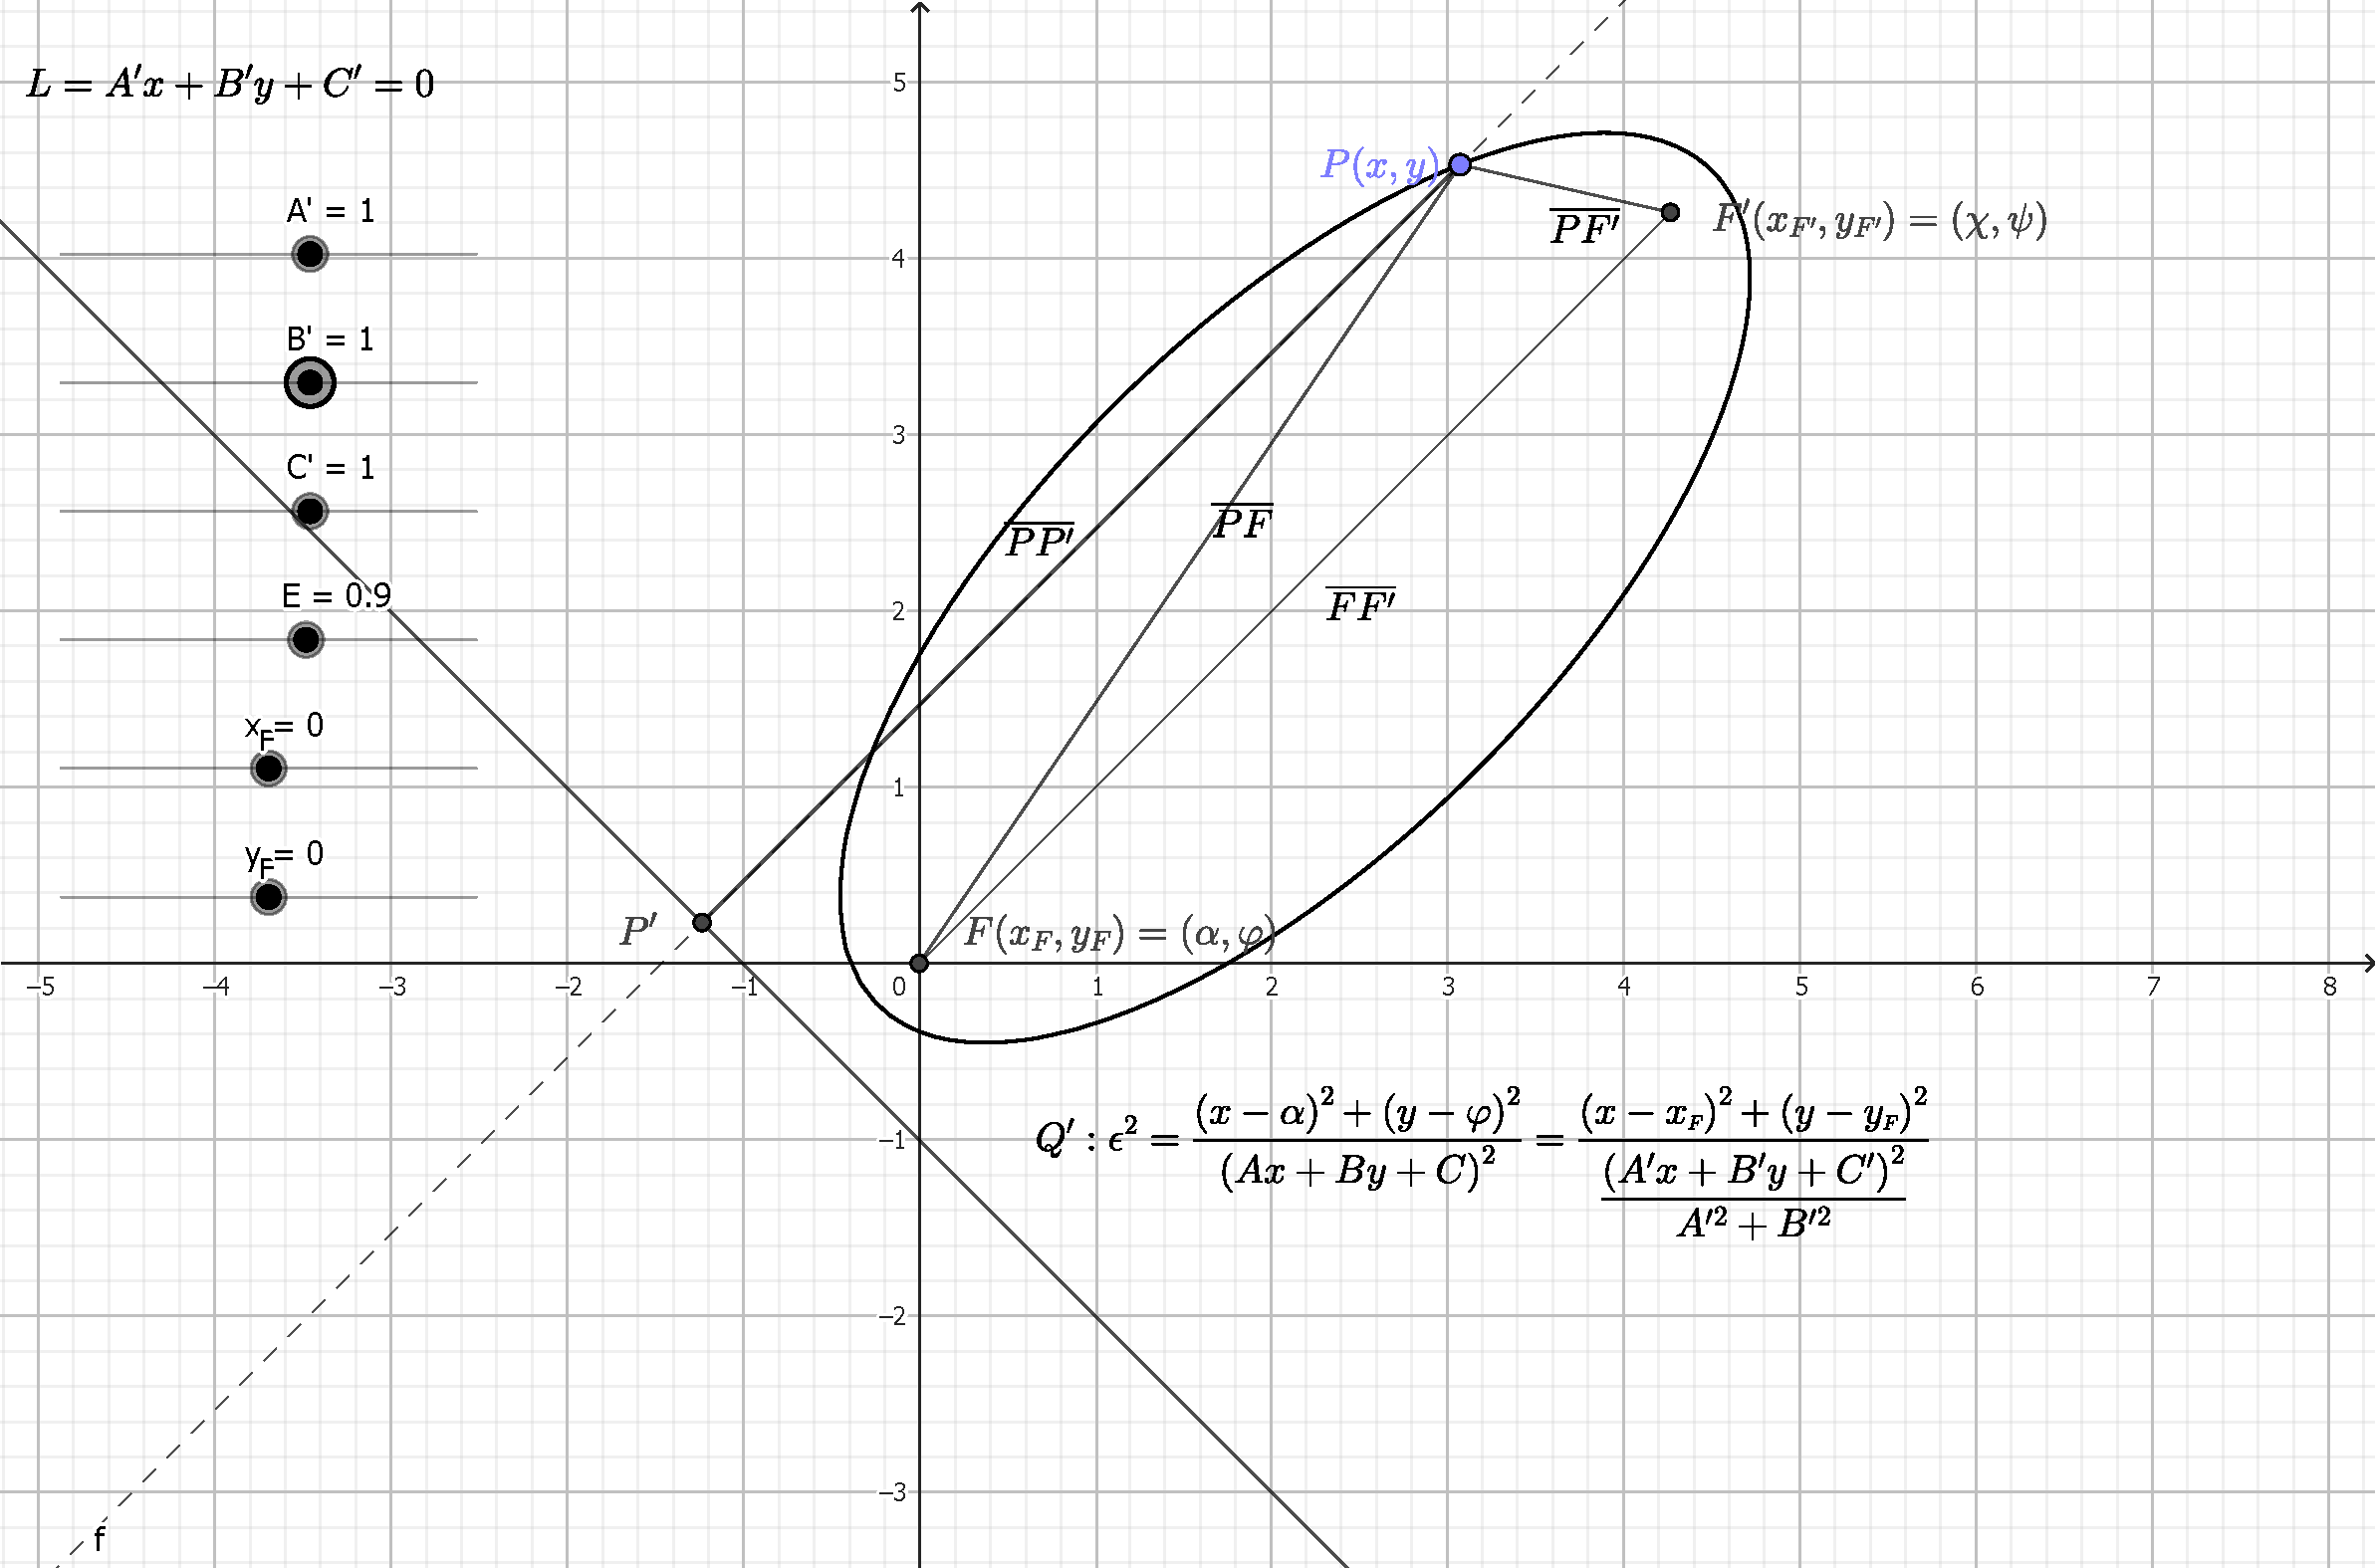
\includegraphics[width=0.75\linewidth]{img/conic-sections} \caption{conic sections}\label{fig:unnamed-chunk-6}
\end{figure}

\url{https://stackoverflow.com/questions/34064292/is-it-possible-to-include-svg-image-in-pdf-document-rendered-by-rmarkdown}

\begin{Shaded}
\begin{Highlighting}[]
\NormalTok{***}
\end{Highlighting}
\end{Shaded}

horizontal rule (or slide break)

\begin{center}\rule{0.5\linewidth}{0.5pt}\end{center}

\begin{Shaded}
\begin{Highlighting}[]
\FunctionTok{dim}\NormalTok{(iris) }
\end{Highlighting}
\end{Shaded}

\begin{verbatim}
## [1] 150   5
\end{verbatim}

\hypertarget{footnote}{%
\subsection{footnote}\label{footnote}}

\hypertarget{hyperlink}{%
\subsection{hyperlink}\label{hyperlink}}

PDF pandoc internal link will lose focus

\protect\hyperlink{equivalence-relation}{equivalence relation} {[}\ref{equivalence-relation}{]} \protect\hyperlink{equivalence-relation}{equivalence relation}\footnote{\{\ref{equivalence-relation}\} \protect\hyperlink{equivalence-relation}{equivalence relation}} \protect\hyperlink{equivalence-relation}{equivalence relation}\textsuperscript{{[}\ref{equivalence-relation}{]}}

\protect\hyperlink{equivalence-class}{equivalence class} {[}\ref{equivalence-class}{]} \protect\hyperlink{equivalence-class}{equivalence class}\footnote{\{\ref{equivalence-class}\} \protect\hyperlink{equivalence-class}{equivalence class}} \protect\hyperlink{equivalence-class}{equivalence class}\textsuperscript{{[}\ref{equivalence-class}{]}}

\protect\hyperlink{partition}{partition} {[}\ref{partition}{]} \protect\hyperlink{partition}{partition}\footnote{\{\ref{partition}\} \protect\hyperlink{partition}{partition}} \protect\hyperlink{partition}{partition}\textsuperscript{{[}\ref{partition}{]}}

\begin{itemize}
\tightlist
\item
  LaTeX

  \begin{itemize}
  \tightlist
  \item
    \protect\hyperlink{tikz}{TikZ}\textsuperscript{{[}\ref{tikz}{]}}

    \begin{itemize}
    \tightlist
    \item
      TikZ-3Dplot
    \item
      PGFplots
    \end{itemize}
  \item
    xypic = \protect\hyperlink{xy-pic}{xy-pic}\footnote{\{\ref{xy-pic}\} \protect\hyperlink{xy-pic}{xy-pic}}
  \end{itemize}
\item
  OverLeaf
\item
  MathCha
\item
  GeoGebra
\item
  Python

  \begin{itemize}
  \tightlist
  \item
    MatPlotLib
  \item
    Seaborn
  \item
    Plotly
  \end{itemize}
\end{itemize}

\hypertarget{xaringan}{%
\subsection{xaringan}\label{xaringan}}

slide realtime preview with RStudio addin Infinite Moon Reader in RStudio viewer

\url{https://github.com/yihui/xaringan}

\url{https://www.youtube.com/watch?v=3n9nASHg9gc}

\hypertarget{bookdown}{%
\section{Bookdown}\label{bookdown}}

\hypertarget{system-locale}{%
\subsection{system locale}\label{system-locale}}

\url{https://bookdown.org/tpemartin/ntpu-programming-for-data-science/appendix-d-.html}

\begin{verbatim}
Sys.getlocale()
\end{verbatim}

Windows

\begin{verbatim}
Sys.setlocale(category = "LC_ALL", locale = "UTF-8")
\end{verbatim}

MacOS

\begin{verbatim}
Sys.setlocale(category = "LC_ALL", locale = "en_US.UTF-8")
\end{verbatim}

\url{https://bookdown.org/yihui/rmarkdown-cookbook/multi-column.html}

\hypertarget{render_book}{%
\subsection{\texorpdfstring{\texttt{render\_book()}}{render\_book()}}\label{render_book}}

\url{https://bookdown.org/yihui/bookdown/build-the-book.html}

\begin{verbatim}
render_book(input = ".", output_format = NULL, ..., clean = TRUE,
  envir = parent.frame(), clean_envir = !interactive(),
  output_dir = NULL, new_session = NA, preview = FALSE,
  config_file = "_bookdown.yml")
\end{verbatim}

\hypertarget{serve_book}{%
\subsection{\texorpdfstring{\texttt{serve\_book()}}{serve\_book()}}\label{serve_book}}

\url{https://bookdown.org/yihui/bookdown/serve-the-book.html}

\begin{verbatim}
serve_book(dir = ".", output_dir = "_book", preview = TRUE,
  in_session = TRUE, quiet = FALSE, ...)
\end{verbatim}

\hypertarget{latex-1}{%
\subsection{LaTeX}\label{latex-1}}

\hypertarget{hyperlink-url-href}{%
\subsubsection{hyperlink, URL, href}\label{hyperlink-url-href}}

\url{https://www.baeldung.com/cs/latex-hyperref-url-hyperlinks}

\begin{CJK}{UTF8}{bsmi}
https://www.omdte.com/小技巧讓-facebook和-line顯示中文網址,網址不再變亂碼/
\end{CJK}

\hypertarget{ugly-mathptmx-sum}{%
\subsubsection{\texorpdfstring{ugly mathptmx \(\sum\)}{ugly mathptmx \textbackslash sum}}\label{ugly-mathptmx-sum}}

PDF LaTeX \texttt{\textbackslash{}usepackage\{fdsymbol\}} to have \texttt{\textbackslash{}overrightharpoon} vector; however, there are too many side effects, including ugly mathptmx \(\sum\), \ldots{}

\begin{verbatim}

\usepackage{fdsymbol} % vector over accent, but will use mathptmx
% replace the rather ugly mathptmx \sum operator with the equivalent Computer Modern one
\let\sum\relax
\DeclareSymbolFont{CMlargesymbols}{OMX}{cmex}{m}{n}
\DeclareMathSymbol{\sum}{\mathop}{CMlargesymbols}{"50}
\end{verbatim}

\url{https://tex.stackexchange.com/questions/315102/different-sum-signs}

\url{https://tex.stackexchange.com/questions/275038/how-to-replace-mathptmx-sum-with-cm-sum}

\url{https://tex.stackexchange.com/questions/391410/calligraphic-symbols-are-too-fancy-with-mathptmx-package}

\url{https://blog.csdn.net/kongtaoxing/article/details/131005044}

In \texttt{preamble.tex}, add

\begin{verbatim}

% replace the rather ugly mathptmx \sum operator with the equivalent Computer Modern one
\let\sum\relax
\DeclareSymbolFont{CMlargesymbols}{OMX}{cmex}{m}{n}
\DeclareMathSymbol{\sum}{\mathop}{CMlargesymbols}{"50}

\DeclareMathAlphabet{\mathcal}{OMS}{cmsy}{m}{n}
\DeclareSymbolFont{largesymbols}{OMX}{cmex}{m}{n}
\end{verbatim}

\hypertarget{latex-package-in-html-document}{%
\subsubsection{LaTeX package in HTML document}\label{latex-package-in-html-document}}

\url{https://github.com/rstudio/rmarkdown/issues/1829}

\begin{verbatim}
---
title: "assignment"
author: "author"
output: html_document
---

$$
  \require{cancel}
  \cancel{x}
$$
\end{verbatim}

\[
  \cancel{x}
\]

\url{https://stackoverflow.com/questions/18189175/how-to-use-textup-with-mathjax}

\texttt{\textbackslash{}textup} is not available in MathJax. You can replace it with \texttt{\textbackslash{}mathrm}, \textbf{but \texttt{\textbackslash{}mathrm} does not interpret spaces}.

\hypertarget{two-columns}{%
\subsection{Two columns}\label{two-columns}}

Below is a Div containing three child Divs side by side. The Div
in the middle is empty, just to add more space between the left
and right Divs.

\begin{verbatim}
:::::: {.cols data-latex=""}

::: {.col data-latex="{0.55\textwidth}"}
![](202401280001-test_files/figure-latex/unnamed-chunk-10-1.pdf)<!-- --> 
:::

::: {.col data-latex="{0.05\textwidth}"}
\ 
<!-- an empty Div (with a white space), serving as
a column separator -->
:::

::: {.col data-latex="{0.4\textwidth}"}
The figure on the left-hand side shows the `cars` data.

Lorem ipsum dolor sit amet, consectetur adipiscing elit, sed do
eiusmod tempor incididunt ut labore et dolore magna aliqua. Ut
enim ad minim veniam, quis nostrud exercitation ullamco laboris
nisi ut aliquip ex ea commodo consequat. Duis aute irure dolor
in reprehenderit in voluptate velit esse cillum dolore eu fugiat
nulla pariatur.
:::
::::::
\end{verbatim}

\begin{cols}

\begin{col}{0.55\textwidth}
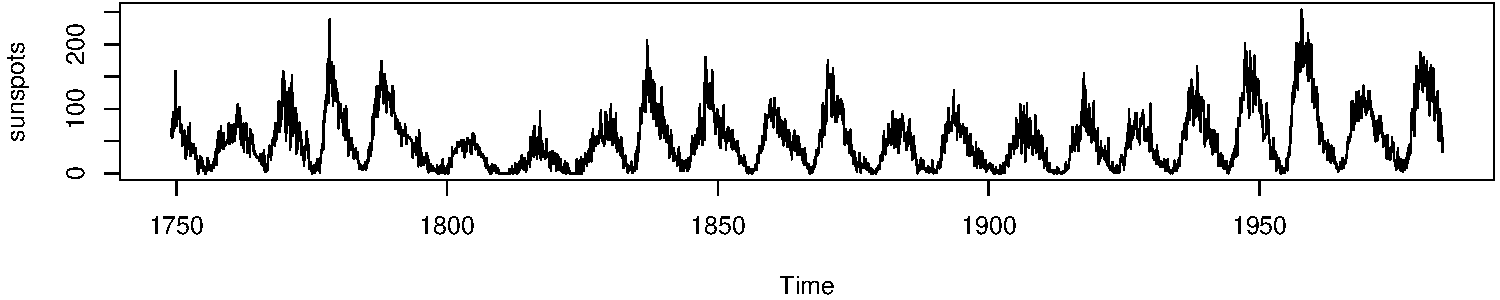
\includegraphics{202401280001-test_files/figure-latex/unnamed-chunk-11-1.pdf}

\end{col}

\begin{col}{0.05\textwidth}
~


\end{col}

\begin{col}{0.4\textwidth}
The figure on the left-hand side shows the \texttt{cars} data.

Lorem ipsum dolor sit amet, consectetur adipiscing elit, sed do
eiusmod tempor incididunt ut labore et dolore magna aliqua. Ut
enim ad minim veniam, quis nostrud exercitation ullamco laboris
nisi ut aliquip ex ea commodo consequat. Duis aute irure dolor
in reprehenderit in voluptate velit esse cillum dolore eu fugiat
nulla pariatur.

\end{col}

\end{cols}

\begin{cols}

\begin{col}{0.55\textwidth}
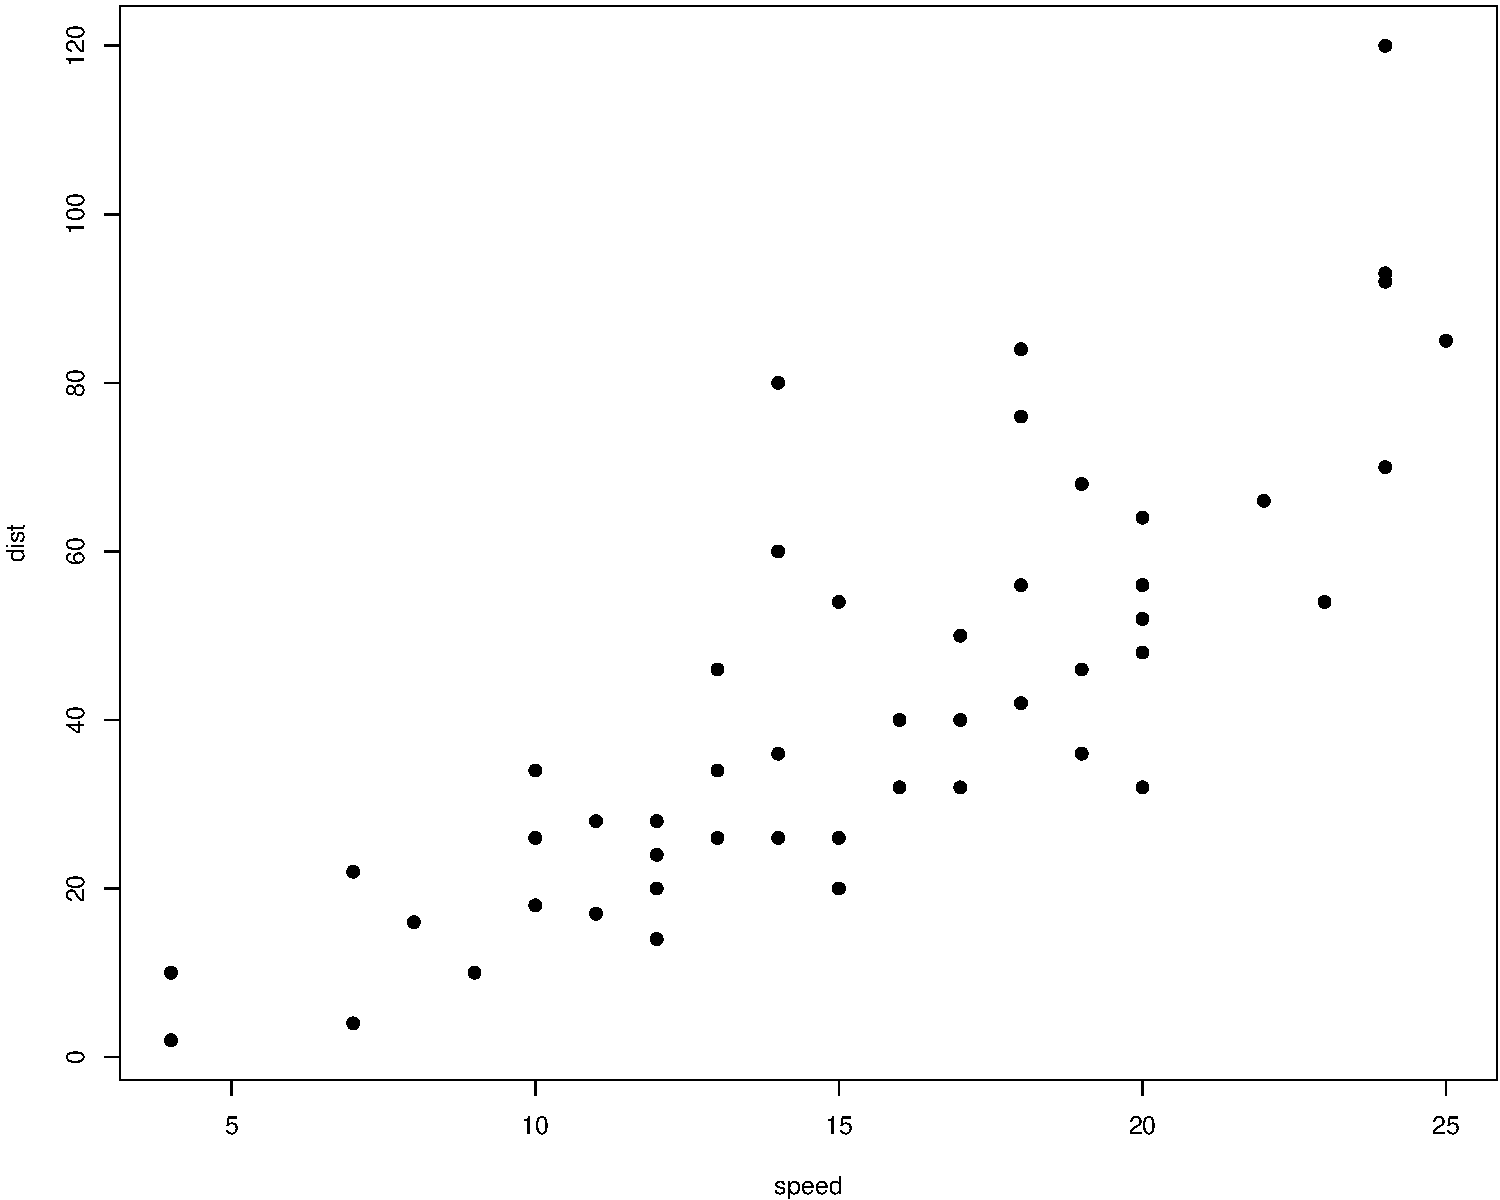
\includegraphics{202401280001-test_files/figure-latex/unnamed-chunk-12-1.pdf}

\end{col}

\begin{col}{0.05\textwidth}
~


\end{col}

\begin{col}{0.4\textwidth}
The figure on the left-hand side shows the \texttt{cars} data.

Lorem ipsum dolor sit amet, consectetur adipiscing elit, sed do
eiusmod tempor incididunt ut labore et dolore magna aliqua. Ut
enim ad minim veniam, quis nostrud exercitation ullamco laboris
nisi ut aliquip ex ea commodo consequat. Duis aute irure dolor
in reprehenderit in voluptate velit esse cillum dolore eu fugiat
nulla pariatur.

\end{col}

\end{cols}

\hypertarget{conditional-blockchunk-for-either-html-or-pdf-and-chinese-issue}{%
\section{conditional block/chunk for either HTML or PDF, and Chinese issue}\label{conditional-blockchunk-for-either-html-or-pdf-and-chinese-issue}}

\url{https://stackoverflow.com/questions/76240244/bookdown-conditional-display-of-text-and-code-blocks-latex-pdf-vs-html}

\begin{CJK}{UTF8}{bsmi}等價關係 equivalence relation \label{def:equivalence-relation}
\end{CJK}
\begin{CJK}{UTF8}{bsmi}
\begin{align*}
 & R\text{ is an equivalence relation over }A\times B\\
\Leftrightarrow & \begin{cases}
R=\sim=\left\{ \left\langle x,y\right\rangle \middle|x\sim y\right\} \subseteq A\times B & \left(\text{e}\right)\text{equivalence 等價}\\
\vdots & \vdots
\end{cases}\\
\Leftrightarrow & \begin{cases}
R=\left\{ \left\langle x,y\right\rangle \middle|xRy\right\} \subseteq A\times B & \left(R\right)\text{relation}\\
\forall\left\langle x,y\right\rangle \in R\left(xRx\right) & \left(r\right)\text{reflexive}\\
\forall\left\langle x,y\right\rangle \in R\left(xRy\Rightarrow yRx\right) & \left(s\right)\text{symmetric}\\
\forall\left\langle x,y\right\rangle ,\left\langle y,z\right\rangle \in R\left(\begin{cases}
xRy\\
yRz
\end{cases}\Rightarrow xRz\right) & \left(t\right)\text{transitive}
\end{cases}\Leftrightarrow\begin{cases}
R=\left\{ \left\langle x,y\right\rangle \middle|xRy\right\} \subseteq A\times B & \text{關係}\\
\forall\left\langle x,y\right\rangle \in R\left(\left\langle x,x\right\rangle \in R\right) & \text{自反}\\
\forall\left\langle x,y\right\rangle \in R\left(\left\langle y,x\right\rangle \in R\right) & \text{對稱}\\
\forall\left\langle x,y\right\rangle ,\left\langle y,z\right\rangle \in R\left(\left\langle x,z\right\rangle \in R\right) & \text{遞移}
\end{cases}
\end{align*}
\end{CJK}

\hypertarget{video-embedding}{%
\section{video embedding}\label{video-embedding}}

\url{https://stackoverflow.com/questions/42543206/r-markdown-compile-error}

always\_allow\_html: true

\begin{Shaded}
\begin{Highlighting}[]
\FunctionTok{install.packages}\NormalTok{(}\StringTok{"webshot"}\NormalTok{)}
\NormalTok{webshot}\SpecialCharTok{::}\FunctionTok{install\_phantomjs}\NormalTok{()}
\end{Highlighting}
\end{Shaded}

however webshot not work

Error: cannot find bilibili.com

\url{https://cran.r-project.org/web/packages/vembedr/vignettes/embed.html}

\begin{verbatim}
## embed_youtube("qeMqtt7NFDM")
\end{verbatim}

\hypertarget{timestamp}{%
\subsection{timestamp}\label{timestamp}}

\begin{itemize}
\tightlist
\item
  YouTube: \url{https://www.youtube.com/embed/\%7BvideoID\%7D?start=\%7Bsecond\%7D}
\item
  BiliBili: \url{https://player.bilibili.com/player.html?bvid=\%7BvideoID\%7D\&autoplay=0\&t=\%7Bsecond\%7D}
\end{itemize}

\hypertarget{equation-term-coloring}{%
\section{equation term coloring}\label{equation-term-coloring}}

\hypertarget{font-color}{%
\subsection{font color}\label{font-color}}

RegEx replacement in RStudio for \texttt{\{\textbackslash{}\textbackslash{}color\{(\textbackslash{}w+)\}} in LyX to be replaced with \texttt{\textbackslash{}\textbackslash{}color\{\$1\}\{} in HTML document, and remain the same for PDF document

In HTML document, if no \texttt{\{\}} for text range, only the first following term will take effect

\texttt{\textbackslash{}color\{orange\}x=y}

\[\color{orange}x=y\]
\texttt{\textbackslash{}color\{orange\}} and \texttt{\textbackslash{}color\{cyan\}} are better color for HTML GitBook \texttt{White} and \texttt{Night} themes and PDF

\texttt{\textbackslash{}color\{cyan\}\{x=y\}}

\[\color{orange}{x=y}\]

\texttt{\textbackslash{}color\{cyan\}\{x=y\}}

\[\color{cyan}{x=y}\]

\begin{verbatim}
::: {show-in="html"}

$$
\begin{aligned}
\color{orange}{\left(A\boldsymbol{x}_{1}\right)^{\intercal}\boldsymbol{x}_{2}}=\left(\boldsymbol{x}_{1}^{\intercal}A^{\intercal}\right)\boldsymbol{x}_{2}\overset{\text{symmetric}}{=} & \left(\boldsymbol{x}_{1}^{\intercal}A\right)\boldsymbol{x}_{2}=\color{orange}{\boldsymbol{x}_{1}^{\intercal}\left(A\boldsymbol{x}_{2}\right)}\\
\left(L\right)=\color{orange}{\left(A\boldsymbol{x}_{1}\right)^{\intercal}\boldsymbol{x}_{2}=} & \color{orange}{\boldsymbol{x}_{1}^{\intercal}\left(A\boldsymbol{x}_{2}\right)}
=\left(R\right)\\
\left(L\right)=\color{orange}{\left(A\boldsymbol{x}_{1}\right)^{\intercal}\boldsymbol{x}_{2}}
\overset{\left(e_{1}\right)}{=} & \left(\lambda_{1}\boldsymbol{x}_{1}\right)^{\intercal}\boldsymbol{x}_{2}=\lambda_{1}\boldsymbol{x}_{1}^{\intercal}\boldsymbol{x}_{2}\\
\left(R\right)=\color{orange}{\boldsymbol{x}_{1}^{\intercal}\left(A\boldsymbol{x}_{2}\right)}\overset{\left(e_{2}\right)}{=} & \boldsymbol{x}_{1}^{\intercal}\left(\lambda_{2}\boldsymbol{x}_{2}\right)=\lambda_{2}\boldsymbol{x}_{1}^{\intercal}\boldsymbol{x}_{2}\\
\lambda_{1}\boldsymbol{x}_{1}^{\intercal}\boldsymbol{x}_{2}=\color{orange}{\left(A\boldsymbol{x}_{1}\right)^{\intercal}\boldsymbol{x}_{2}=} & \color{orange}{\boldsymbol{x}_{1}^{\intercal}\left(A\boldsymbol{x}_{2}\right)}=\lambda_{2}\boldsymbol{x}_{1}^{\intercal}\boldsymbol{x}_{2}\\
\lambda_{1}\boldsymbol{x}_{1}^{\intercal}\boldsymbol{x}_{2}= & \lambda_{2}\boldsymbol{x}_{1}^{\intercal}\boldsymbol{x}_{2}
\end{aligned}
$$

:::

::: {show-in="pdf"}

$$
\begin{aligned}
{\color{orange}\left(A\boldsymbol{x}_{1}\right)^{\intercal}\boldsymbol{x}_{2}}=\left(\boldsymbol{x}_{1}^{\intercal}A^{\intercal}\right)\boldsymbol{x}_{2}\overset{\text{symmetric}}{=} & \left(\boldsymbol{x}_{1}^{\intercal}A\right)\boldsymbol{x}_{2}={\color{orange}\boldsymbol{x}_{1}^{\intercal}\left(A\boldsymbol{x}_{2}\right)}\\
\left(L\right)={\color{orange}\left(A\boldsymbol{x}_{1}\right)^{\intercal}\boldsymbol{x}_{2}=} & {\color{orange}\boldsymbol{x}_{1}^{\intercal}\left(A\boldsymbol{x}_{2}\right)}=\left(R\right)\\
\left(L\right)={\color{orange}\left(A\boldsymbol{x}_{1}\right)^{\intercal}\boldsymbol{x}_{2}}\overset{\left(e_{1}\right)}{=} & \left(\lambda_{1}\boldsymbol{x}_{1}\right)^{\intercal}\boldsymbol{x}_{2}=\lambda_{1}\boldsymbol{x}_{1}^{\intercal}\boldsymbol{x}_{2}\\
\left(R\right)={\color{orange}\boldsymbol{x}_{1}^{\intercal}\left(A\boldsymbol{x}_{2}\right)}\overset{\left(e_{2}\right)}{=} & \boldsymbol{x}_{1}^{\intercal}\left(\lambda_{2}\boldsymbol{x}_{2}\right)=\lambda_{2}\boldsymbol{x}_{1}^{\intercal}\boldsymbol{x}_{2}\\
\lambda_{1}\boldsymbol{x}_{1}^{\intercal}\boldsymbol{x}_{2}={\color{orange}\left(A\boldsymbol{x}_{1}\right)^{\intercal}\boldsymbol{x}_{2}=} & {\color{orange}\boldsymbol{x}_{1}^{\intercal}\left(A\boldsymbol{x}_{2}\right)}=\lambda_{2}\boldsymbol{x}_{1}^{\intercal}\boldsymbol{x}_{2}\\
\lambda_{1}\boldsymbol{x}_{1}^{\intercal}\boldsymbol{x}_{2}= & \lambda_{2}\boldsymbol{x}_{1}^{\intercal}\boldsymbol{x}_{2}
\end{aligned}
$$

:::
\end{verbatim}

\hypertarget{background-color}{%
\subsection{background color}\label{background-color}}

\url{https://bookdown.org/yihui/rmarkdown-cookbook/font-color.html}

LaTex color

\url{https://latexcolor.com/}

\url{https://www.overleaf.com/learn/latex/Using_colors_in_LaTeX}

\url{https://latex-tutorial.com/color-latex/\#}:\textasciitilde:text=To\%20summarize\%2C\%20pyellow!50efined\%20colors\%20in,when\%20loading\%20the\%20xcolor\%20package.

LaTex color methods

color frame

\url{https://tex.stackexchange.com/questions/582748/highlight-equation-with-boxes-and-arrows}

color box

\url{https://tex.stackexchange.com/questions/567739/how-to-move-and-size-colorbox}

color box with round corners

\url{https://tex.stackexchange.com/questions/568880/color-box-with-rounded-corners}

highlighting

\url{https://tex.stackexchange.com/questions/318991/highlighting-math}

\url{https://forum.remnote.io/t/highlighting-latex-formulas/149}

LyX

\url{https://tex.stackexchange.com/questions/250069/create-a-color-box}
\url{https://latexlyx.blogspot.com/2013/12/lyx.html}

\url{https://tex.stackexchange.com/questions/635486/prevent-lyx-from-escaping-math-in-color-box-title}

Bookdown - conditional display of text and code blocks (LaTeX/PDF vs.~HTML)
\url{https://stackoverflow.com/questions/76240244/bookdown-conditional-display-of-text-and-code-blocks-latex-pdf-vs-html}

\begin{align*}
\colorbox{yellow!50}{$F$}= & \colorbox{yellow!50}{$ma$}\\
\end{align*}

\url{https://community.rstudio.com/t/highlighting-text-inline-in-rmarkdown-or-bookdown-pdf/35118/4}
\definecolor{hightlightColor}{HTML}{FFFF66}

\begin{align*}
\colorbox{hightlightColor}{$F$}= & \colorbox{yellow!50}{$ma$}\\
\end{align*}

\begin{align*}
\colorbox{hightlightColor}{\ensuremath{F}}= & \colorbox{yellow!50}{\ensuremath{F}}\\
\end{align*}

\begin{equation}
\colorbox{yellow!50}{$F$}=\colorbox{yellow!50}{$ma$}
\end{equation}

\[
\colorbox{hightlightColor}{$F$}=\colorbox{yellow!50}{$ma$}
\]

\[
\colorbox{yellow!50}{$Y = \beta_0 + \beta_1 X_1 + \ldots + \beta_n X_n$}
\]

\hypertarget{link-and-reference}{%
\section{link and reference}\label{link-and-reference}}

\url{https://stackoverflow.com/questions/57469501/cross-referencing-bookdownhtml-document2-not-working}

\begin{equation}
  E=mc^2
  \label{eq:emc}
\end{equation}

\texttt{\textbackslash{}@ref(nice-label)} \ref{nice-label}

\texttt{{[}link\ to\ partition{]}{[}partition{]}} \protect\hyperlink{partition}{link to partition}

\texttt{{[}partition{]}} \texttt{\textbackslash{}@ref(partition)}

\protect\hyperlink{partition}{partition} {[}\#partition{]} (\ref{partition}) @ref(\#partition)

\texttt{{[}equivalence\ class{]}} \texttt{\textbackslash{}@ref(equivalence\ class)}

\protect\hyperlink{equivalence-class}{equivalence class} {[}\#equivalence class{]} (@ref(equivalence class)) @ref(\#equivalence class)

{[}equivalence-class{]} {[}\#equivalence-class{]} (\ref{equivalence-class}) @ref(\#equivalence-class)

{[}equivalence-class.html{]} {[}equivalence-class.html\#equivalence-class{]} (@ref(equivalence-class.html)) @ref(equivalence-class.html\#equivalence-class)

\protect\hyperlink{equivalence-relation}{equivalence relation} {[}\#equivalence relation{]} (@ref(equivalence relation)) @ref(\#equivalence relation)

{[}equivalence-relation{]} {[}\#equivalence-relation{]} (\ref{equivalence-relation}) @ref(\#equivalence-relation)

{[}equivalence-relation.html{]} {[}equivalence-relation.html\#equivalence-relation{]} (@ref(equivalence-relation.html)) @ref(equivalence-relation.html\#equivalence-relation)

\hypertarget{number-and-reference-equations}{%
\section{number and reference equations}\label{number-and-reference-equations}}

\url{https://stackoverflow.com/questions/71595882/rstudio-error-in-windows-running-pdflatex-exe-on-file-name-tex-exit-code-10}

\url{https://bookdown.org/yihui/rmarkdown/bookdown-markdown.html\#equations}

\texttt{\textbackslash{}\#eq:emc}
\texttt{\textbackslash{}@ref(eq:emc)}

\url{https://stackoverflow.com/questions/55923290/consistent-math-equation-numbering-in-bookdown-across-pdf-docx-html-output}

\begin{equation}
\begin{aligned}
 & C\text{ is an equivalence class of }a\text{ on }A\\
\Leftrightarrow & \left[a\right]_{\sim}=C=\left\{ x\middle|\begin{cases}
a\in A\\
x\in A\\
x\sim a\\
\sim\text{ is an equivalence relation over }A\times A=A^{2}
\end{cases}\right\} \subseteq A\ne\emptyset\\
\Leftrightarrow & \left[a\right]=\left[a\right]_{\sim}=\left\{ x\middle|\begin{cases}
a\in A\\
x\in A\\
x\sim a\\
\sim\text{ is an equivalence relation on }A
\end{cases}\right\} \subseteq A\ne\emptyset\\
\Rightarrow & \left[a\right]_{\sim}=\left\{ x\middle|x\sim a\right\} \subseteq A\ne\emptyset
\end{aligned}
\label{eq:eqclass}
\end{equation}

\url{https://bookdown.org/yihui/rmarkdown/bookdown-markdown.html\#cross-referencing}

This cross reference is the Fig. \ref{fig:parabola-arc-with-points}

\url{https://stackoverflow.com/questions/51595939/bookdown-cross-reference-figure-in-another-file}

I ran into the same issue and came up with this solution if you aim at compiling 2 different pdfs. It relies on LaTeX's xr package for cross references: \url{https://stackoverflow.com/a/52532269/576684}

\hypertarget{footnote-1}{%
\section{footnote}\label{footnote-1}}

noun\footnote{This is a footnote.}

\hypertarget{citation}{%
\section{citation}\label{citation}}

\url{https://stackoverflow.com/questions/48965247/use-csl-file-for-pdf-output-in-bookdown/49145699\#49145699}

citation 1\textsuperscript{\protect\hyperlink{ref-noauthor_bookdown_2019}{3}} citation 2\textsuperscript{\protect\hyperlink{ref-noauthor_bookdown_2019}{3}}

citation 3\textsuperscript{\protect\hyperlink{ref-ccjou2009}{4}} citation 4\textsuperscript{\protect\hyperlink{ref-ccjou2009}{4}}

\hypertarget{backreference}{%
\subsection{backreference}\label{backreference}}

\url{https://community.rstudio.com/t/how-to-create-a-backreference-to-place-of-citation-in-rmarkdown/84866}

\url{https://blog.csdn.net/RobertChenGuangzhi/article/details/50455429}

\url{https://latex.org/forum/viewtopic.php?t=3722}

\hypertarget{bookdown-environment-for-definition-theorem-proof}{%
\section{bookdown environment for definition, theorem, proof}\label{bookdown-environment-for-definition-theorem-proof}}

\url{https://bookdown.org/yihui/rmarkdown/bookdown-markdown.html}

\url{https://github.com/rstudio/rstudio/issues/5264}

\texttt{@howthebodyworks} Ideally, previews of such equations should also work inside a theorem, although I could survive without that.

\url{https://github.com/rstudio/rstudio/issues/8773}

\begin{theorem}[Theorem Name]
\protect\hypertarget{thm:label}{}\label{thm:label}Here is my theorem.
\end{theorem}

\begin{proof}[Proof Name]
Here is my proof.
\end{proof}

\begin{theorem}[Pythagorean theorem]
\protect\hypertarget{thm:pyth}{}\label{thm:pyth}For a right triangle, if \(c\) denotes the length of the hypotenuse
and \(a\) and \(b\) denote the lengths of the other two sides, we have

\[a^2 + \color{cyan}b^2 \overset{\ref{eq:emc}}= \color{red}{c^2} \]
\end{theorem}

\begin{definition}[Definition Name]
\protect\hypertarget{def:unnamed-chunk-22}{}\label{def:unnamed-chunk-22}Here is my definition.
\end{definition}

\protect\hyperlink{number-and-reference-equations}{number and reference equations}

\eqref{eq:eqclass}

\eqref{eq:emc}

\ref{thm:pyth}

\begin{figure}
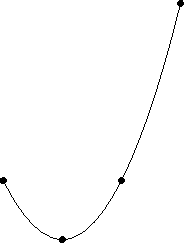
\includegraphics[width=0.25\linewidth]{202401280001-test_files/figure-latex/parabola-arc-with-points-1} \caption{parabola arc with points}\label{fig:parabola-arc-with-points}
\end{figure}

\hypertarget{test2}{%
\chapter{test2}\label{test2}}

\hypertarget{verbatim}{%
\section{verbatim}\label{verbatim}}

\url{https://bookdown.org/yihui/rmarkdown-cookbook/verbatim-code-chunks.html}

\begin{Shaded}
\begin{Highlighting}[]

\NormalTok{\textasciigrave{}\textasciigrave{}\textasciigrave{}r}
\NormalTok{1 + 1}
\NormalTok{\textasciigrave{}\textasciigrave{}\textasciigrave{}}

\NormalTok{\textasciigrave{}\textasciigrave{}\textasciigrave{}}
\NormalTok{\#\# [1] 2}
\NormalTok{\textasciigrave{}\textasciigrave{}\textasciigrave{}}
\end{Highlighting}
\end{Shaded}

\begin{Shaded}
\begin{Highlighting}[]
\NormalTok{We can output arbitrary content **verbatim**.}


\InformationTok{\textasciigrave{}\textasciigrave{}\textasciigrave{}r}
\DecValTok{1} \SpecialCharTok{+} \DecValTok{1}
\InformationTok{\textasciigrave{}\textasciigrave{}\textasciigrave{}}

\InformationTok{\textasciigrave{}\textasciigrave{}\textasciigrave{}}
\InformationTok{\#\# [1] 2}
\InformationTok{\textasciigrave{}\textasciigrave{}\textasciigrave{}}

\NormalTok{The content can contain inline code like}
\NormalTok{78.5398163, too.}
\end{Highlighting}
\end{Shaded}

\hypertarget{partition}{%
\chapter{partition}\label{partition}}

\begin{align*}
 & \left\{ A_{i}\right\} _{i\in I}=\left\{ A_{i}\middle|i\in I\right\} \text{ is a partition of a set }A\\
\Leftrightarrow & \begin{cases}
\forall i\in I\left(A_{i}\ne\emptyset\right)\\
A=\bigcup\limits _{i\in I}A_{i}\\
\forall i,j\in I\left(i\ne j\Rightarrow A_{i}\cap A_{j}=\emptyset\right)
\end{cases}
\end{align*}

\url{https://proofwiki.org/wiki/Definition:Set_Partition}

\hypertarget{equivalence-class}{%
\chapter{equivalence class}\label{equivalence-class}}

\begin{align*}
 & C\text{ is an equivalence class of }a\text{ on }A\\
\Leftrightarrow & \left[a\right]_{\sim}=C=\left\{ x\middle|\begin{cases}
a\in A\\
x\in A\\
x\sim a\\
\sim\text{ is an equivalence relation over }A\times A=A^{2}
\end{cases}\right\} \subseteq A\ne\emptyset\\
\Leftrightarrow & \left[a\right]=\left[a\right]_{\sim}=\left\{ x\middle|\begin{cases}
a\in A\\
x\in A\\
x\sim a\\
\sim\text{ is an equivalence relation on }A
\end{cases}\right\} \subseteq A\ne\emptyset\\
\Rightarrow & \left[a\right]_{\sim}=\left\{ x\middle|x\sim a\right\} \subseteq A\ne\emptyset
\end{align*}

where the definition of \protect\hyperlink{equivalence-relation}{equivalence relation} can be found in \ref{equivalence-relation}.

\hypertarget{equivalence-relation}{%
\chapter{equivalence relation}\label{equivalence-relation}}

\begin{CJK}{UTF8}{bsmi}等價關係 equivalence relation \label{def:equivalence-relation}
\end{CJK}
\begin{CJK}{UTF8}{bsmi}
\begin{align*}
 & R\text{ is an equivalence relation over }A\times B\\
\Leftrightarrow & \begin{cases}
R=\sim=\left\{ \left\langle x,y\right\rangle \middle|x\sim y\right\} \subseteq A\times B & \left(\text{e}\right)\text{equivalence 等價}\\
\vdots & \vdots
\end{cases}\\
\Leftrightarrow & \begin{cases}
R=\left\{ \left\langle x,y\right\rangle \middle|xRy\right\} \subseteq A\times B & \left(R\right)\text{relation}\\
\forall\left\langle x,y\right\rangle \in R\left(xRx\right) & \left(r\right)\text{reflexive}\\
\forall\left\langle x,y\right\rangle \in R\left(xRy\Rightarrow yRx\right) & \left(s\right)\text{symmetric}\\
\forall\left\langle x,y\right\rangle ,\left\langle y,z\right\rangle \in R\left(\begin{cases}
xRy\\
yRz
\end{cases}\Rightarrow xRz\right) & \left(t\right)\text{transitive}
\end{cases}\Leftrightarrow\begin{cases}
R=\left\{ \left\langle x,y\right\rangle \middle|xRy\right\} \subseteq A\times B & \text{關係}\\
\forall\left\langle x,y\right\rangle \in R\left(\left\langle x,x\right\rangle \in R\right) & \text{自反}\\
\forall\left\langle x,y\right\rangle \in R\left(\left\langle y,x\right\rangle \in R\right) & \text{對稱}\\
\forall\left\langle x,y\right\rangle ,\left\langle y,z\right\rangle \in R\left(\left\langle x,z\right\rangle \in R\right) & \text{遞移}
\end{cases}
\end{align*}
\end{CJK}

\hypertarget{python}{%
\chapter{Python}\label{python}}

\url{https://bookdown.org/yihui/rmarkdown/language-engines.html}

\begin{Shaded}
\begin{Highlighting}[]
\FunctionTok{names}\NormalTok{(knitr}\SpecialCharTok{::}\NormalTok{knit\_engines}\SpecialCharTok{$}\FunctionTok{get}\NormalTok{())}
\end{Highlighting}
\end{Shaded}

\begin{verbatim}
##  [1] "awk"         "bash"        "coffee"      "gawk"        "groovy"     
##  [6] "haskell"     "lein"        "mysql"       "node"        "octave"     
## [11] "perl"        "php"         "psql"        "Rscript"     "ruby"       
## [16] "sas"         "scala"       "sed"         "sh"          "stata"      
## [21] "zsh"         "asis"        "asy"         "block"       "block2"     
## [26] "bslib"       "c"           "cat"         "cc"          "comment"    
## [31] "css"         "ditaa"       "dot"         "embed"       "eviews"     
## [36] "exec"        "fortran"     "fortran95"   "go"          "highlight"  
## [41] "js"          "julia"       "python"      "R"           "Rcpp"       
## [46] "sass"        "scss"        "sql"         "stan"        "targets"    
## [51] "tikz"        "verbatim"    "theorem"     "lemma"       "corollary"  
## [56] "proposition" "conjecture"  "definition"  "example"     "exercise"   
## [61] "hypothesis"  "proof"       "remark"      "solution"
\end{verbatim}

\url{https://rstudio.github.io/reticulate/articles/python_packages.html}

\begin{Shaded}
\begin{Highlighting}[]
\NormalTok{x }\OperatorTok{=} \StringTok{\textquotesingle{}hello, python world!\textquotesingle{}}
\BuiltInTok{print}\NormalTok{(x.split(}\StringTok{\textquotesingle{} \textquotesingle{}}\NormalTok{))}
\end{Highlighting}
\end{Shaded}

\begin{verbatim}
## ['hello,', 'python', 'world!']
\end{verbatim}

\begin{Shaded}
\begin{Highlighting}[]
\FunctionTok{library}\NormalTok{(reticulate)}
\FunctionTok{virtualenv\_python}\NormalTok{()}
\end{Highlighting}
\end{Shaded}

\begin{Shaded}
\begin{Highlighting}[]
\FunctionTok{library}\NormalTok{(reticulate)}
\CommentTok{\# conda\_list()}
\end{Highlighting}
\end{Shaded}

\begin{Shaded}
\begin{Highlighting}[]
\FunctionTok{library}\NormalTok{(reticulate)}
\FunctionTok{virtualenv\_list}\NormalTok{()}
\end{Highlighting}
\end{Shaded}

\url{https://rstudio.github.io/reticulate/reference/install_python.html}

\begin{Shaded}
\begin{Highlighting}[]
\FunctionTok{library}\NormalTok{(reticulate)}
\NormalTok{version }\OtherTok{\textless{}{-}} \StringTok{"3.9.12"}
\CommentTok{\# install\_python(version)}

\CommentTok{\# create a new environment}
\CommentTok{\# virtualenv\_create("r{-}reticulate", version = version)}

\CommentTok{\# use\_virtualenv("r{-}reticulate")}

\CommentTok{\# install MatPlotLib}
\CommentTok{\# virtualenv\_install("r{-}reticulate", "matplotlib")}

\CommentTok{\# import MatPlotLib (it will be automatically discovered in "r{-}reticulate")}
\NormalTok{matplotlib }\OtherTok{\textless{}{-}} \FunctionTok{import}\NormalTok{(}\StringTok{"matplotlib"}\NormalTok{)}
\end{Highlighting}
\end{Shaded}

copy \texttt{C:\textbackslash{}Users\textbackslash{}RW\textbackslash{}AppData\textbackslash{}Local\textbackslash{}r-reticulate\textbackslash{}r-reticulate\textbackslash{}pyenv\textbackslash{}pyenv-win\textbackslash{}versions\textbackslash{}3.9.12\textbackslash{}tcl\textbackslash{}tcl8.6} and \texttt{C:\textbackslash{}Users\textbackslash{}RW\textbackslash{}AppData\textbackslash{}Local\textbackslash{}r-reticulate\textbackslash{}r-reticulate\textbackslash{}pyenv\textbackslash{}pyenv-win\textbackslash{}versions\textbackslash{}3.9.12\textbackslash{}tcl\textbackslash{}tk8.6} two folders to the folder \texttt{C:\textbackslash{}Users\textbackslash{}RW\textbackslash{}AppData\textbackslash{}Local\textbackslash{}r-reticulate\textbackslash{}r-reticulate\textbackslash{}pyenv\textbackslash{}pyenv-win\textbackslash{}versions\textbackslash{}3.9.12\textbackslash{}Lib}

\begin{Shaded}
\begin{Highlighting}[]
\CommentTok{\# library(reticulate)}
\CommentTok{\# use\_virtualenv("r{-}reticulate")}
\CommentTok{\# \# matplotlib \textless{}{-} import("matplotlib")}
\CommentTok{\# matplotlib$use("Agg", force = TRUE)}
\end{Highlighting}
\end{Shaded}

\begin{Shaded}
\begin{Highlighting}[]
\ImportTok{import}\NormalTok{ matplotlib.pyplot }\ImportTok{as}\NormalTok{ plt}
\NormalTok{plt.plot([}\DecValTok{0}\NormalTok{, }\DecValTok{2}\NormalTok{, }\DecValTok{1}\NormalTok{, }\DecValTok{4}\NormalTok{])}
\NormalTok{plt.show()}
\end{Highlighting}
\end{Shaded}

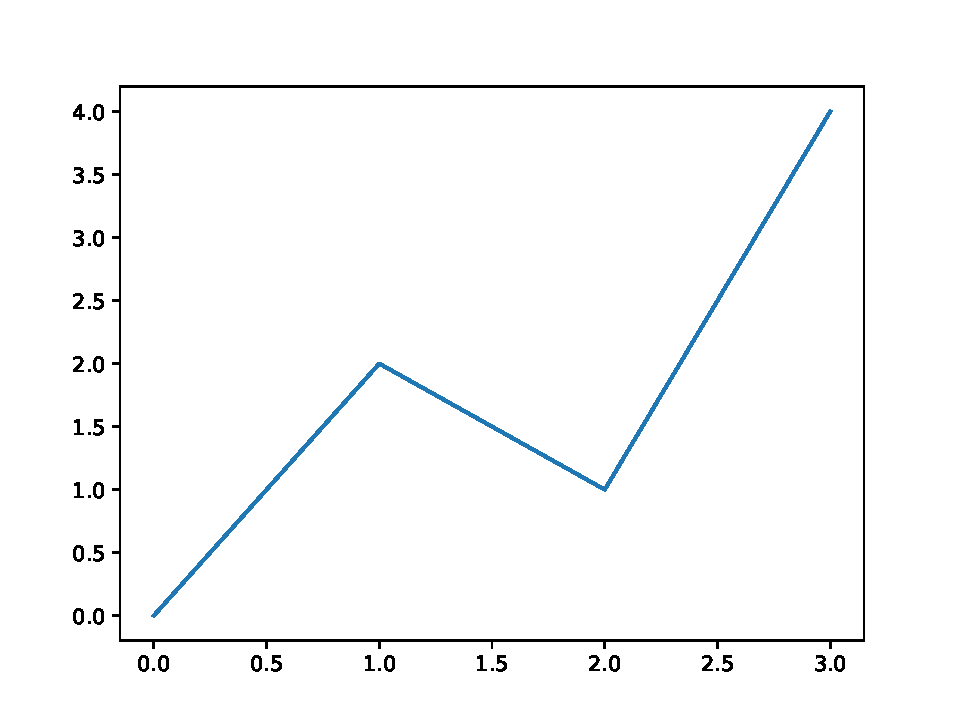
\includegraphics{202401292317-Python_files/figure-latex/unnamed-chunk-8-1.pdf}

\hypertarget{tikz}{%
\chapter{TikZ}\label{tikz}}

\protect\hyperlink{two-columns}{two columns} {[}\ref{two-columns}{]}

\begin{cols}

\begin{col}{0.4\textwidth}

\begin{Shaded}
\begin{Highlighting}[]
\KeywordTok{\textbackslash{}begin}\NormalTok{\{}\ExtensionTok{tikzpicture}\NormalTok{\}}
  \FunctionTok{\textbackslash{}draw}\NormalTok{ ({-}1,1){-}{-}(0,0){-}{-}(1,2);}
\KeywordTok{\textbackslash{}end}\NormalTok{\{}\ExtensionTok{tikzpicture}\NormalTok{\}}
\end{Highlighting}
\end{Shaded}

\end{col}

\begin{col}{0.05\textwidth}
~


\end{col}

\begin{col}{0.55\textwidth}
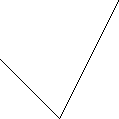
\includegraphics{202401311000-TikZ_files/figure-latex/unnamed-chunk-2-1.pdf}

\end{col}

\end{cols}

How to speed up bookdown generation?

\url{https://stackoverflow.com/questions/56541371/how-to-speed-up-bookdown-generation}

TikZ and PGFplots

What's the relation between packages PGFplots and TikZ?

\url{https://tex.stackexchange.com/questions/285925/whats-the-relation-between-packages-pgfplots-and-tikz}

\url{https://www.youtube.com/watch?v=bQugbYq0BVA}

\url{https://www.youtube.com/watch?v=ft4Kg9emK1k\&list=PLg5nrpKdkk2DWcg3scb75AknF7DJXs8lk\&index=18}

\begin{Shaded}
\begin{Highlighting}[]
\KeywordTok{\textbackslash{}begin}\NormalTok{\{}\ExtensionTok{tikzpicture}\NormalTok{\}}
  \FunctionTok{\textbackslash{}def\textbackslash{}a}\NormalTok{\{1.5\} }\CommentTok{\% amplitude}
  \FunctionTok{\textbackslash{}def\textbackslash{}b}\NormalTok{\{2\}   }\CommentTok{\% frequency}
  \FunctionTok{\textbackslash{}draw}\NormalTok{[{-}\textgreater{}] ({-}0.2,0){-}{-}(4.2,0) node[right, font=}\FunctionTok{\textbackslash{}small}\NormalTok{] \{}\SpecialStringTok{$x$}\NormalTok{\};}
  \FunctionTok{\textbackslash{}draw}\NormalTok{[{-}\textgreater{}] (0,{-}4){-}{-}(0,0.5) node[above] \{}\SpecialStringTok{$y$}\NormalTok{\};}
  \FunctionTok{\textbackslash{}draw}\NormalTok{[domain=0:4,smooth,variable=}\FunctionTok{\textbackslash{}t}\NormalTok{,blue,thick] }
\NormalTok{    plot (\{}\FunctionTok{\textbackslash{}a}\NormalTok{ * (}\FunctionTok{\textbackslash{}b*\textbackslash{}t}\NormalTok{ {-} sin(deg(}\FunctionTok{\textbackslash{}b*\textbackslash{}t}\NormalTok{)))\},\{{-}}\FunctionTok{\textbackslash{}a}\NormalTok{ * (1 {-} cos(deg(}\FunctionTok{\textbackslash{}b*\textbackslash{}t}\NormalTok{)))\});}
  \CommentTok{\% \textbackslash{}node[above] at (2, 0.5) \{Brachistochrone Curve\};}
  \FunctionTok{\textbackslash{}node}\NormalTok{[above, font=}\FunctionTok{\textbackslash{}footnotesize}\NormalTok{] at (2, 1) \{Brachistochrone Curve\};}
  \FunctionTok{\textbackslash{}node}\NormalTok{[above, font=}\FunctionTok{\textbackslash{}footnotesize}\NormalTok{] at (2, 0) \{}\SpecialStringTok{$}\KeywordTok{\textbackslash{}begin}\NormalTok{\{}\ExtensionTok{aligned}\NormalTok{\}}
\SpecialStringTok{\& x=r(t{-}}\SpecialCharTok{\textbackslash{}sin}\SpecialStringTok{ t) }\SpecialCharTok{\textbackslash{}\textbackslash{}}
\SpecialStringTok{\& y=r(1{-}}\SpecialCharTok{\textbackslash{}cos}\SpecialStringTok{ t)}
\KeywordTok{\textbackslash{}end}\NormalTok{\{}\ExtensionTok{aligned}\NormalTok{\}}\SpecialStringTok{$}\NormalTok{\};}
\KeywordTok{\textbackslash{}end}\NormalTok{\{}\ExtensionTok{tikzpicture}\NormalTok{\}}
\end{Highlighting}
\end{Shaded}

\begin{figure}

\includegraphics[width=0.9\linewidth]{202401311000-TikZ_files/figure-latex/unnamed-chunk-4-1} \caption{Brachistochrone Curve}\label{fig:unnamed-chunk-4}
\end{figure}

\begin{figure}
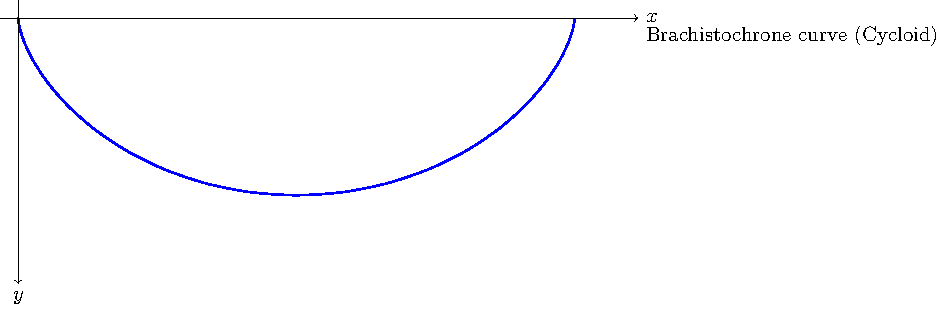
\includegraphics[width=0.9\linewidth]{202401311000-TikZ_files/figure-latex/unnamed-chunk-5-1} \caption{Brachistochrone Curve}\label{fig:unnamed-chunk-5}
\end{figure}

\hypertarget{d}{%
\section{2D}\label{d}}

\url{https://zhuanlan.zhihu.com/p/127155579?utm_psn=1741479950987960320}

\begin{Shaded}
\begin{Highlighting}[]
\KeywordTok{\textbackslash{}begin}\NormalTok{\{}\ExtensionTok{tikzpicture}\NormalTok{\}}
  \FunctionTok{\textbackslash{}draw}\NormalTok{ ({-}1,1){-}{-}(0,0){-}{-}(1,2);}
\KeywordTok{\textbackslash{}end}\NormalTok{\{}\ExtensionTok{tikzpicture}\NormalTok{\}}
\end{Highlighting}
\end{Shaded}

\begin{figure}
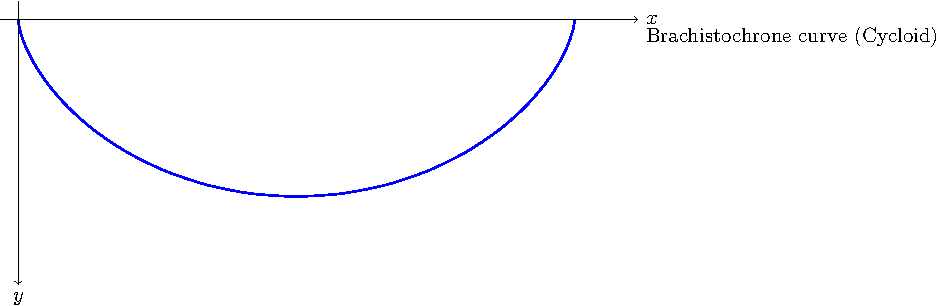
\includegraphics[width=0.05\linewidth]{202401311000-TikZ_files/figure-latex/unnamed-chunk-7-1} \end{figure}

\begin{figure}
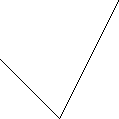
\includegraphics[width=0.05\linewidth]{202401311000-TikZ_files/figure-latex/unnamed-chunk-8-1} \end{figure}

\begin{figure}
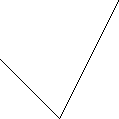
\includegraphics[width=0.2\linewidth]{202401311000-TikZ_files/figure-latex/unnamed-chunk-9-1} \end{figure}

2

\begin{figure}

\includegraphics[width=0.15\linewidth]{202401311000-TikZ_files/figure-latex/unnamed-chunk-10-1} \end{figure}

3

\begin{figure}
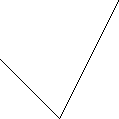
\includegraphics[width=0.25\linewidth]{202401311000-TikZ_files/figure-latex/unnamed-chunk-11-1} \end{figure}

\begin{Shaded}
\begin{Highlighting}[]
\KeywordTok{\textbackslash{}begin}\NormalTok{\{}\ExtensionTok{tikzpicture}\NormalTok{\}}
  \FunctionTok{\textbackslash{}draw}\NormalTok{[rounded corners] ({-}1,1){-}{-}(0,0){-}{-}(1,2){-}{-}({-}1,1);}
\KeywordTok{\textbackslash{}end}\NormalTok{\{}\ExtensionTok{tikzpicture}\NormalTok{\}}
\end{Highlighting}
\end{Shaded}

\begin{figure}
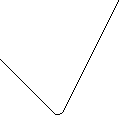
\includegraphics[width=0.25\linewidth]{202401311000-TikZ_files/figure-latex/unnamed-chunk-13-1} \caption{rounded corner pseudo-closed triangle}\label{fig:unnamed-chunk-13}
\end{figure}

\begin{Shaded}
\begin{Highlighting}[]
\KeywordTok{\textbackslash{}begin}\NormalTok{\{}\ExtensionTok{tikzpicture}\NormalTok{\}}
  \FunctionTok{\textbackslash{}draw}\NormalTok{[rounded corners] ({-}1,1){-}{-}(0,0){-}{-}(1,2){-}{-}cycle;}
\KeywordTok{\textbackslash{}end}\NormalTok{\{}\ExtensionTok{tikzpicture}\NormalTok{\}}
\end{Highlighting}
\end{Shaded}

\begin{figure}
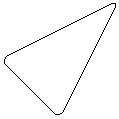
\includegraphics[width=0.25\linewidth]{202401311000-TikZ_files/figure-latex/unnamed-chunk-15-1} \caption{rounded corner triangle}\label{fig:unnamed-chunk-15}
\end{figure}

\begin{figure}
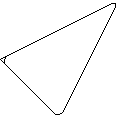
\includegraphics[width=0.25\linewidth]{202401311000-TikZ_files/figure-latex/unnamed-chunk-16-1} \caption{triangle vs. pseudo-closed triangle}\label{fig:unnamed-chunk-16}
\end{figure}

\begin{Shaded}
\begin{Highlighting}[]
\KeywordTok{\textbackslash{}begin}\NormalTok{\{}\ExtensionTok{tikzpicture}\NormalTok{\}}
  \FunctionTok{\textbackslash{}draw}\NormalTok{ (0,0) rectangle (4,2);}
\KeywordTok{\textbackslash{}end}\NormalTok{\{}\ExtensionTok{tikzpicture}\NormalTok{\}}
\end{Highlighting}
\end{Shaded}

\begin{figure}
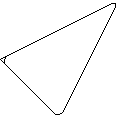
\includegraphics[width=0.25\linewidth]{202401311000-TikZ_files/figure-latex/unnamed-chunk-18-1} \caption{rectangle}\label{fig:unnamed-chunk-18}
\end{figure}

\begin{Shaded}
\begin{Highlighting}[]
\KeywordTok{\textbackslash{}begin}\NormalTok{\{}\ExtensionTok{tikzpicture}\NormalTok{\}}
  \FunctionTok{\textbackslash{}draw}\NormalTok{ (0,0) rectangle (2,2);}
\KeywordTok{\textbackslash{}end}\NormalTok{\{}\ExtensionTok{tikzpicture}\NormalTok{\}}
\end{Highlighting}
\end{Shaded}

\begin{figure}

\includegraphics[width=0.25\linewidth]{202401311000-TikZ_files/figure-latex/unnamed-chunk-20-1} \caption{square}\label{fig:unnamed-chunk-20}
\end{figure}

\begin{Shaded}
\begin{Highlighting}[]
\KeywordTok{\textbackslash{}begin}\NormalTok{\{}\ExtensionTok{tikzpicture}\NormalTok{\}}
  \FunctionTok{\textbackslash{}draw}\NormalTok{ (0,0) circle (1);}
\KeywordTok{\textbackslash{}end}\NormalTok{\{}\ExtensionTok{tikzpicture}\NormalTok{\}}
\end{Highlighting}
\end{Shaded}

\begin{figure}

\includegraphics[width=0.25\linewidth]{202401311000-TikZ_files/figure-latex/unnamed-chunk-22-1} \caption{circle}\label{fig:unnamed-chunk-22}
\end{figure}

\begin{Shaded}
\begin{Highlighting}[]
\KeywordTok{\textbackslash{}begin}\NormalTok{\{}\ExtensionTok{tikzpicture}\NormalTok{\}}
  \FunctionTok{\textbackslash{}draw}\NormalTok{ (0,0) circle (1);}
  \FunctionTok{\textbackslash{}draw}\NormalTok{ (0,0) rectangle (2,2);}
\KeywordTok{\textbackslash{}end}\NormalTok{\{}\ExtensionTok{tikzpicture}\NormalTok{\}}
\end{Highlighting}
\end{Shaded}

\begin{figure}

\includegraphics[width=0.25\linewidth]{202401311000-TikZ_files/figure-latex/unnamed-chunk-24-1} \caption{circle and square}\label{fig:unnamed-chunk-24}
\end{figure}

\begin{Shaded}
\begin{Highlighting}[]
\KeywordTok{\textbackslash{}begin}\NormalTok{\{}\ExtensionTok{tikzpicture}\NormalTok{\}}
  \FunctionTok{\textbackslash{}draw}\NormalTok{ (1,1) ellipse (2 and 1);}
\KeywordTok{\textbackslash{}end}\NormalTok{\{}\ExtensionTok{tikzpicture}\NormalTok{\}}
\end{Highlighting}
\end{Shaded}

\begin{figure}
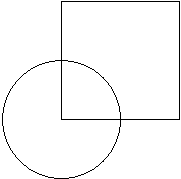
\includegraphics[width=0.25\linewidth]{202401311000-TikZ_files/figure-latex/unnamed-chunk-26-1} \caption{ellipse}\label{fig:unnamed-chunk-26}
\end{figure}

\begin{Shaded}
\begin{Highlighting}[]
\KeywordTok{\textbackslash{}begin}\NormalTok{\{}\ExtensionTok{tikzpicture}\NormalTok{\}}
  \FunctionTok{\textbackslash{}draw}\NormalTok{ (1 ,1) arc (0:270:1);}
  \FunctionTok{\textbackslash{}draw}\NormalTok{ (6 ,1) arc (0:270:2 and 1);}
\KeywordTok{\textbackslash{}end}\NormalTok{\{}\ExtensionTok{tikzpicture}\NormalTok{\}}
\end{Highlighting}
\end{Shaded}

\begin{figure}
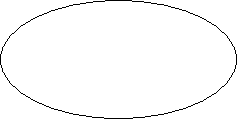
\includegraphics[width=0.25\linewidth]{202401311000-TikZ_files/figure-latex/unnamed-chunk-28-1} \caption{circle and ellipse arcs}\label{fig:unnamed-chunk-28}
\end{figure}

\begin{Shaded}
\begin{Highlighting}[]
\KeywordTok{\textbackslash{}begin}\NormalTok{\{}\ExtensionTok{tikzpicture}\NormalTok{\}}
  \FunctionTok{\textbackslash{}draw}\NormalTok{ ({-}1,1) parabola bend (0,0) (2,4);}
\KeywordTok{\textbackslash{}end}\NormalTok{\{}\ExtensionTok{tikzpicture}\NormalTok{\}}
\end{Highlighting}
\end{Shaded}

\begin{figure}

\includegraphics[width=0.25\linewidth]{202401311000-TikZ_files/figure-latex/unnamed-chunk-30-1} \caption{parabola arc}\label{fig:unnamed-chunk-30}
\end{figure}

\begin{Shaded}
\begin{Highlighting}[]
\KeywordTok{\textbackslash{}begin}\NormalTok{\{}\ExtensionTok{tikzpicture}\NormalTok{\}}
  \FunctionTok{\textbackslash{}draw}\NormalTok{ ({-}1,1) parabola bend (0,0) (2,4);}
  \FunctionTok{\textbackslash{}filldraw}
\NormalTok{    ({-}1,1) circle (.05)}
\NormalTok{    ( 0,0) circle (.05)}
\NormalTok{    ( 1,1) circle (.05)}
\NormalTok{    ( 2,4) circle (.05);}
\KeywordTok{\textbackslash{}end}\NormalTok{\{}\ExtensionTok{tikzpicture}\NormalTok{\}}
\end{Highlighting}
\end{Shaded}

\begin{figure}

\includegraphics[width=0.25\linewidth]{202401311000-TikZ_files/figure-latex/unnamed-chunk-32-1} \caption{parabola arc with points}\label{fig:unnamed-chunk-32}
\end{figure}

\begin{Shaded}
\begin{Highlighting}[]
\KeywordTok{\textbackslash{}begin}\NormalTok{\{}\ExtensionTok{tikzpicture}\NormalTok{\}}
  \FunctionTok{\textbackslash{}draw}\NormalTok{[step=20pt] (0,0) grid (3,2);}
  \FunctionTok{\textbackslash{}draw}\NormalTok{[help lines ,step=20pt] (4,0) grid (7,2);}
\KeywordTok{\textbackslash{}end}\NormalTok{\{}\ExtensionTok{tikzpicture}\NormalTok{\}}
\end{Highlighting}
\end{Shaded}

\begin{figure}
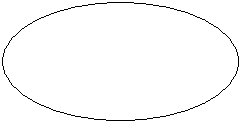
\includegraphics[width=0.75\linewidth]{202401311000-TikZ_files/figure-latex/unnamed-chunk-34-1} \caption{grid and help lines}\label{fig:unnamed-chunk-34}
\end{figure}

\begin{figure}

\includegraphics[width=0.75\linewidth]{202401311000-TikZ_files/figure-latex/unnamed-chunk-35-1} \caption{grid and help lines}\label{fig:unnamed-chunk-35}
\end{figure}

\begin{Shaded}
\begin{Highlighting}[]
\KeywordTok{\textbackslash{}begin}\NormalTok{\{}\ExtensionTok{tikzpicture}\NormalTok{\}[scale=0.25]}
  \FunctionTok{\textbackslash{}draw}\NormalTok{[{-}\textgreater{}] (0,0){-}{-}(9,0);}
  \FunctionTok{\textbackslash{}draw}\NormalTok{[\textless{}{-}] (0,1){-}{-}(9,1);}
  \FunctionTok{\textbackslash{}draw}\NormalTok{[\textless{}{-}\textgreater{}] (0,2){-}{-}(9,2);}
  \FunctionTok{\textbackslash{}draw}\NormalTok{[\textgreater{}{-}\textgreater{}\textgreater{}] (0,3){-}{-}(9,3);}
  \FunctionTok{\textbackslash{}draw}\NormalTok{[|\textless{}{-}\textgreater{}|] (0,4){-}{-}(9,4);}
\KeywordTok{\textbackslash{}end}\NormalTok{\{}\ExtensionTok{tikzpicture}\NormalTok{\}}
\end{Highlighting}
\end{Shaded}

\begin{figure}

\includegraphics[width=0.75\linewidth]{202401311000-TikZ_files/figure-latex/unnamed-chunk-37-1} \caption{arrows}\label{fig:unnamed-chunk-37}
\end{figure}

\begin{Shaded}
\begin{Highlighting}[]
\KeywordTok{\textbackslash{}begin}\NormalTok{\{}\ExtensionTok{tikzpicture}\NormalTok{\}}
  \FunctionTok{\textbackslash{}draw}\NormalTok{[line width =2pt] (0,6){-}{-}(9,6); }
  \FunctionTok{\textbackslash{}draw}\NormalTok{[dotted]          (0,5){-}{-}(9,5); }
  \FunctionTok{\textbackslash{}draw}\NormalTok{[densely dotted]  (0,4){-}{-}(9,4); }
  \FunctionTok{\textbackslash{}draw}\NormalTok{[loosely dotted]  (0,3){-}{-}(9,3); }
  \FunctionTok{\textbackslash{}draw}\NormalTok{[dashed]          (0,2){-}{-}(9,2); }
  \FunctionTok{\textbackslash{}draw}\NormalTok{[densely dashed]  (0,1){-}{-}(9,1); }
  \FunctionTok{\textbackslash{}draw}\NormalTok{[loosely dashed]  (0,0){-}{-}(9,0);}
\KeywordTok{\textbackslash{}end}\NormalTok{\{}\ExtensionTok{tikzpicture}\NormalTok{\}}
\end{Highlighting}
\end{Shaded}

\begin{figure}
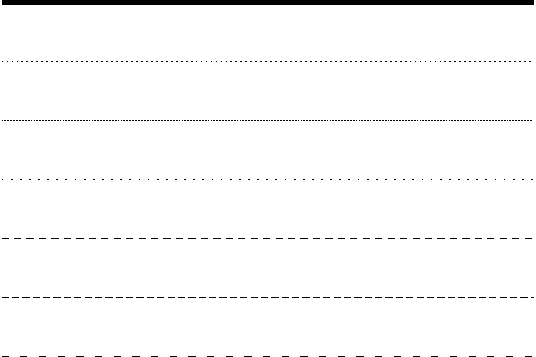
\includegraphics[width=0.75\linewidth]{202401311000-TikZ_files/figure-latex/unnamed-chunk-39-1} \caption{arrows}\label{fig:unnamed-chunk-39}
\end{figure}

\begin{Shaded}
\begin{Highlighting}[]
\KeywordTok{\textbackslash{}begin}\NormalTok{\{}\ExtensionTok{tikzpicture}\NormalTok{\}[dline/.style=\{color= blue, line width=2pt\}]}
  \FunctionTok{\textbackslash{}draw}\NormalTok{[dline] (0,0){-}{-}(9,0); }
\KeywordTok{\textbackslash{}end}\NormalTok{\{}\ExtensionTok{tikzpicture}\NormalTok{\}}
\end{Highlighting}
\end{Shaded}

\begin{figure}

\includegraphics[width=0.75\linewidth]{202401311000-TikZ_files/figure-latex/unnamed-chunk-41-1} \caption{head styling}\label{fig:unnamed-chunk-41}
\end{figure}

\begin{Shaded}
\begin{Highlighting}[]
\KeywordTok{\textbackslash{}begin}\NormalTok{\{}\ExtensionTok{tikzpicture}\NormalTok{\}}
  \FunctionTok{\textbackslash{}draw}\NormalTok{ (0,0) rectangle (2,2);}
  \FunctionTok{\textbackslash{}draw}\NormalTok{[shift=\{( 3, 0)\}] (0,0) rectangle (2,2);}
  \FunctionTok{\textbackslash{}draw}\NormalTok{[shift=\{( 0, 3)\}] (0,0) rectangle (2,2);}
  \FunctionTok{\textbackslash{}draw}\NormalTok{[shift=\{( 0,{-}3)\}] (0,0) rectangle (2,2);}
  \FunctionTok{\textbackslash{}draw}\NormalTok{[shift=\{({-}3, 0)\}] (0,0) rectangle (2,2);}
  \FunctionTok{\textbackslash{}draw}\NormalTok{[shift=\{( 3, 3)\}] (0,0) rectangle (2,2);}
  \FunctionTok{\textbackslash{}draw}\NormalTok{[shift=\{({-}3, 3)\}] (0,0) rectangle (2,2);}
  \FunctionTok{\textbackslash{}draw}\NormalTok{[shift=\{( 3,{-}3)\}] (0,0) rectangle (2,2);}
  \FunctionTok{\textbackslash{}draw}\NormalTok{[shift=\{({-}3,{-}3)\}] (0,0) rectangle (2,2);}
\KeywordTok{\textbackslash{}end}\NormalTok{\{}\ExtensionTok{tikzpicture}\NormalTok{\}}
\end{Highlighting}
\end{Shaded}

\begin{figure}

\includegraphics[width=0.75\linewidth]{202401311000-TikZ_files/figure-latex/unnamed-chunk-43-1} \caption{transform: shift}\label{fig:unnamed-chunk-43}
\end{figure}

\begin{Shaded}
\begin{Highlighting}[]
\KeywordTok{\textbackslash{}begin}\NormalTok{\{}\ExtensionTok{tikzpicture}\NormalTok{\}}
  \FunctionTok{\textbackslash{}draw}\NormalTok{ (0,0) rectangle (2,2);}
  \FunctionTok{\textbackslash{}draw}\NormalTok{[xshift= 100pt] (0,0) rectangle (2,2);}
  \FunctionTok{\textbackslash{}draw}\NormalTok{[xshift={-}100pt] (0,0) rectangle (2,2);}
  \FunctionTok{\textbackslash{}draw}\NormalTok{[yshift= 100pt] (0,0) rectangle (2,2);}
  \FunctionTok{\textbackslash{}draw}\NormalTok{[yshift={-}100pt] (0,0) rectangle (2,2);}
\KeywordTok{\textbackslash{}end}\NormalTok{\{}\ExtensionTok{tikzpicture}\NormalTok{\}}
\end{Highlighting}
\end{Shaded}

\begin{figure}

\includegraphics[width=0.75\linewidth]{202401311000-TikZ_files/figure-latex/unnamed-chunk-45-1} \caption{transform: shift x, y}\label{fig:unnamed-chunk-45}
\end{figure}

\begin{Shaded}
\begin{Highlighting}[]
\KeywordTok{\textbackslash{}begin}\NormalTok{\{}\ExtensionTok{tikzpicture}\NormalTok{\}}
  \FunctionTok{\textbackslash{}draw}\NormalTok{ (0,0) rectangle (2,2);}
  \FunctionTok{\textbackslash{}draw}\NormalTok{[xshift= 100pt, xscale=1.5] (0,0) rectangle (2,2);}
  \FunctionTok{\textbackslash{}draw}\NormalTok{[yshift= 100pt, xscale=0.5] (0,0) rectangle (2,2);}
  \FunctionTok{\textbackslash{}draw}\NormalTok{[xshift={-}100pt, yscale=1.5] (0,0) rectangle (2,2);}
  \FunctionTok{\textbackslash{}draw}\NormalTok{[yshift={-}100pt, yscale=0.5] (0,0) rectangle (2,2);}
\KeywordTok{\textbackslash{}end}\NormalTok{\{}\ExtensionTok{tikzpicture}\NormalTok{\}}
\end{Highlighting}
\end{Shaded}

\begin{figure}

\includegraphics[width=0.75\linewidth]{202401311000-TikZ_files/figure-latex/unnamed-chunk-47-1} \caption{transform: scale x, y}\label{fig:unnamed-chunk-47}
\end{figure}

\begin{Shaded}
\begin{Highlighting}[]
\KeywordTok{\textbackslash{}begin}\NormalTok{\{}\ExtensionTok{tikzpicture}\NormalTok{\}}
  \FunctionTok{\textbackslash{}draw}\NormalTok{ (0,0) rectangle (2,2);}
  \FunctionTok{\textbackslash{}draw}\NormalTok{[xshift= 100pt, xscale=1.5] (0,0) rectangle (2,2);}
  \FunctionTok{\textbackslash{}draw}\NormalTok{[yshift= 100pt, yscale=1.5] (0,0) rectangle (2,2);}
  \FunctionTok{\textbackslash{}draw}\NormalTok{[xshift={-}100pt, xscale=0.5] (0,0) rectangle (2,2);}
  \FunctionTok{\textbackslash{}draw}\NormalTok{[yshift={-}100pt, yscale=0.5] (0,0) rectangle (2,2);}
\KeywordTok{\textbackslash{}end}\NormalTok{\{}\ExtensionTok{tikzpicture}\NormalTok{\}}
\end{Highlighting}
\end{Shaded}

\begin{figure}

\includegraphics[width=0.75\linewidth]{202401311000-TikZ_files/figure-latex/unnamed-chunk-49-1} \caption{transform: scale}\label{fig:unnamed-chunk-49}
\end{figure}

\begin{Shaded}
\begin{Highlighting}[]
\KeywordTok{\textbackslash{}begin}\NormalTok{\{}\ExtensionTok{tikzpicture}\NormalTok{\}}
  \FunctionTok{\textbackslash{}draw}\NormalTok{ (0,0) rectangle (2,2);}
  \FunctionTok{\textbackslash{}draw}\NormalTok{[xshift=125pt,rotate=45] (0,0) rectangle (2,2);}
  \FunctionTok{\textbackslash{}draw}\NormalTok{[xshift=175pt,rotate around=\{45:(2 ,2)\}] (0,0) rectangle (2,2);}
\KeywordTok{\textbackslash{}end}\NormalTok{\{}\ExtensionTok{tikzpicture}\NormalTok{\}}
\end{Highlighting}
\end{Shaded}

\begin{figure}
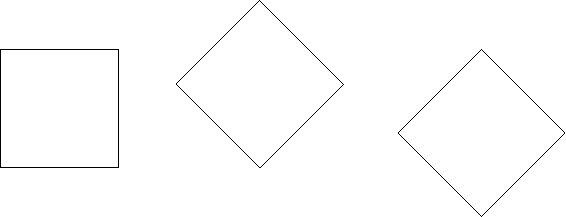
\includegraphics[width=0.75\linewidth]{202401311000-TikZ_files/figure-latex/unnamed-chunk-51-1} \caption{transform: rotate}\label{fig:unnamed-chunk-51}
\end{figure}

\begin{Shaded}
\begin{Highlighting}[]
\KeywordTok{\textbackslash{}begin}\NormalTok{\{}\ExtensionTok{tikzpicture}\NormalTok{\}}
  \FunctionTok{\textbackslash{}draw}\NormalTok{ (0,0) rectangle (2,2);}
  \FunctionTok{\textbackslash{}draw}\NormalTok{[xshift=70pt,xslant=1] (0,0) rectangle (2,2);}
  \FunctionTok{\textbackslash{}draw}\NormalTok{[yshift=70pt,yslant=1] (0,0) rectangle (2,2);}
\KeywordTok{\textbackslash{}end}\NormalTok{\{}\ExtensionTok{tikzpicture}\NormalTok{\}}
\end{Highlighting}
\end{Shaded}

\begin{figure}

\includegraphics[width=0.75\linewidth]{202401311000-TikZ_files/figure-latex/unnamed-chunk-53-1} \caption{transform: slant}\label{fig:unnamed-chunk-53}
\end{figure}

\begin{Shaded}
\begin{Highlighting}[]
\FunctionTok{\textbackslash{}tikzset}\NormalTok{\{}
\NormalTok{  box/.style=\{}
\NormalTok{    draw=blue,}
\NormalTok{    rectangle,}
\NormalTok{    rounded corners=5pt,}
\NormalTok{    minimum width=50pt,}
\NormalTok{    minimum height=20pt,}
\NormalTok{    inner sep=5pt}
\NormalTok{  \}}
\NormalTok{\}}
\KeywordTok{\textbackslash{}begin}\NormalTok{\{}\ExtensionTok{tikzpicture}\NormalTok{\}}
  \FunctionTok{\textbackslash{}node}\NormalTok{[box] (1) at (0,0) \{1\};}
  \FunctionTok{\textbackslash{}node}\NormalTok{[box] (2) at (4,0) \{2\};}
  \FunctionTok{\textbackslash{}node}\NormalTok{[box] (3) at (8,0) \{3\};}
  \FunctionTok{\textbackslash{}draw}\NormalTok{[{-}\textgreater{}] (1){-}{-}(2);}
  \FunctionTok{\textbackslash{}draw}\NormalTok{[{-}\textgreater{}] (2){-}{-}(3);}
  \FunctionTok{\textbackslash{}node}\NormalTok{ at (2,1) \{a\};}
  \FunctionTok{\textbackslash{}node}\NormalTok{ at (6,1) \{b\};}
\KeywordTok{\textbackslash{}end}\NormalTok{\{}\ExtensionTok{tikzpicture}\NormalTok{\}}
\end{Highlighting}
\end{Shaded}

\begin{figure}
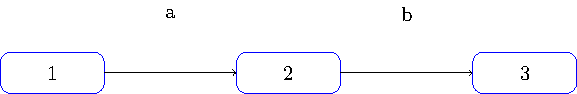
\includegraphics[width=0.75\linewidth]{202401311000-TikZ_files/figure-latex/unnamed-chunk-55-1} \caption{flowchart}\label{fig:unnamed-chunk-55}
\end{figure}

\begin{Shaded}
\begin{Highlighting}[]
\FunctionTok{\textbackslash{}tikzset}\NormalTok{\{}
\NormalTok{  box/.style=\{}
\NormalTok{    draw=blue,}
\NormalTok{    fill=blue!20,}
\NormalTok{    rectangle,}
\NormalTok{    rounded corners=5pt,}
\NormalTok{    minimum height=20pt,}
\NormalTok{    inner sep=5pt}
\NormalTok{  \}}
\NormalTok{\}}
\KeywordTok{\textbackslash{}begin}\NormalTok{\{}\ExtensionTok{tikzpicture}\NormalTok{\}}
  \FunctionTok{\textbackslash{}node}\NormalTok{[box] \{1\}}
\NormalTok{      child \{node[box] \{2\}\}}
\NormalTok{      child \{node[box] \{3\}}
\NormalTok{          child \{node[box] \{4\}\}}
\NormalTok{          child \{node[box] \{5\}\}}
\NormalTok{          child \{node[box] \{6\}\}}
\NormalTok{      \};}
\KeywordTok{\textbackslash{}end}\NormalTok{\{}\ExtensionTok{tikzpicture}\NormalTok{\}}
\end{Highlighting}
\end{Shaded}

\begin{figure}
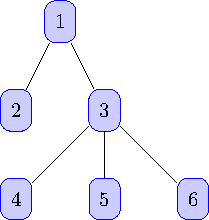
\includegraphics[width=0.75\linewidth]{202401311000-TikZ_files/figure-latex/unnamed-chunk-57-1} \caption{tree}\label{fig:unnamed-chunk-57}
\end{figure}

\begin{Shaded}
\begin{Highlighting}[]
\KeywordTok{\textbackslash{}begin}\NormalTok{\{}\ExtensionTok{tikzpicture}\NormalTok{\}}
  \FunctionTok{\textbackslash{}draw}\NormalTok{[{-}\textgreater{}] ({-}0.2,0){-}{-}(6,0) node[right] \{}\SpecialStringTok{$x$}\NormalTok{\};}
  \FunctionTok{\textbackslash{}draw}\NormalTok{[{-}\textgreater{}] (0,{-}0.2){-}{-}(0,6) node[above] \{}\SpecialStringTok{$f(x)$}\NormalTok{\};}
  \FunctionTok{\textbackslash{}draw}\NormalTok{[domain=0:4] plot (}\FunctionTok{\textbackslash{}x}\NormalTok{ ,\{0.1* exp(}\FunctionTok{\textbackslash{}x}\NormalTok{)\}) node[right] \{}\SpecialStringTok{$f(x)=}\SpecialCharTok{\textbackslash{}frac}\SpecialStringTok{\{1\}\{10\}e\^{}x$}\NormalTok{\};}
\KeywordTok{\textbackslash{}end}\NormalTok{\{}\ExtensionTok{tikzpicture}\NormalTok{\}}
\end{Highlighting}
\end{Shaded}

\begin{figure}
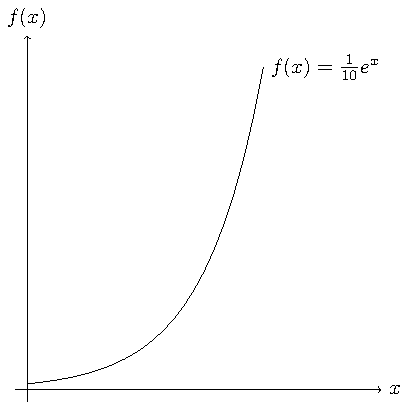
\includegraphics[width=0.75\linewidth]{202401311000-TikZ_files/figure-latex/unnamed-chunk-59-1} \caption{tree}\label{fig:unnamed-chunk-59}
\end{figure}

\url{https://stackoverflow.com/questions/64897575/tikz-libraries-in-bookdown}

It turns out that you can simply put the \texttt{\textbackslash{}usetikzlibrary\{...\}} command directly before the \texttt{\textbackslash{}begin\{tikzpicture\}} and everything works fine :)

\url{https://stackoverflow.com/questions/56211210/r-markdown-document-with-html-docx-output-using-latex-package-bbm}

\url{https://tex.stackexchange.com/questions/171711/how-to-include-latex-package-in-r-markdown}

\hypertarget{d-1}{%
\section{3D}\label{d-1}}

\url{https://zhuanlan.zhihu.com/p/431732330?utm_psn=1741857547550638080}

\url{https://github.com/RRWWW/Stereometry}

\begin{Shaded}
\begin{Highlighting}[]
\KeywordTok{\textbackslash{}begin}\NormalTok{\{}\ExtensionTok{tikzpicture}\NormalTok{\}}
  \FunctionTok{\textbackslash{}coordinate}\NormalTok{ (A) at ( 1, 1, 1);}
  \FunctionTok{\textbackslash{}coordinate}\NormalTok{ (B) at ( 1, 1,{-}1);}
  \FunctionTok{\textbackslash{}coordinate}\NormalTok{ (C) at ( 1,{-}1,{-}1);}
  \FunctionTok{\textbackslash{}coordinate}\NormalTok{ (D) at ( 1,{-}1, 1);}
  \FunctionTok{\textbackslash{}coordinate}\NormalTok{ (E) at ({-}1,{-}1, 1);}
  \FunctionTok{\textbackslash{}coordinate}\NormalTok{ (F) at ({-}1,{-}1,{-}1);}
  \FunctionTok{\textbackslash{}coordinate}\NormalTok{ (G) at ({-}1, 1,{-}1);}
  \FunctionTok{\textbackslash{}coordinate}\NormalTok{ (H) at ({-}1, 1, 1);}
  \FunctionTok{\textbackslash{}draw}\NormalTok{ (A) node[right=1pt] \{}\SpecialStringTok{$A$}\NormalTok{\}{-}{-}}
\NormalTok{        (B) node[right=1pt] \{}\SpecialStringTok{$B$}\NormalTok{\}{-}{-}}
\NormalTok{        (C) node[right=1pt] \{}\SpecialStringTok{$C$}\NormalTok{\}{-}{-}}
\NormalTok{        (D) node[right=1pt] \{}\SpecialStringTok{$D$}\NormalTok{\}{-}{-}}
\NormalTok{        (E) node[left= 1pt] \{}\SpecialStringTok{$E$}\NormalTok{\}{-}{-}}
\NormalTok{        (F) node[right=1pt] \{}\SpecialStringTok{$F$}\NormalTok{\}{-}{-}}
\NormalTok{        (G) node[right=1pt] \{}\SpecialStringTok{$G$}\NormalTok{\}{-}{-}}
\NormalTok{        (H) node[left= 1pt] \{}\SpecialStringTok{$H$}\NormalTok{\}{-}{-}}
\NormalTok{        (A) node[right=1pt] \{}\SpecialStringTok{$A$}\NormalTok{\};}
\KeywordTok{\textbackslash{}end}\NormalTok{\{}\ExtensionTok{tikzpicture}\NormalTok{\}}
\end{Highlighting}
\end{Shaded}

\begin{figure}
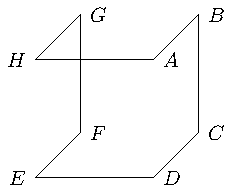
\includegraphics[width=0.75\linewidth]{202401311000-TikZ_files/figure-latex/unnamed-chunk-61-1} \caption{cube}\label{fig:unnamed-chunk-61}
\end{figure}

\begin{Shaded}
\begin{Highlighting}[]
\FunctionTok{\textbackslash{}usetikzlibrary}\NormalTok{\{patterns\}}
\FunctionTok{\textbackslash{}usetikzlibrary}\NormalTok{\{3d,calc\}}
\FunctionTok{\textbackslash{}tdplotsetmaincoords}\NormalTok{\{45\}\{45\}}
\KeywordTok{\textbackslash{}begin}\NormalTok{\{}\ExtensionTok{tikzpicture}\NormalTok{\}[tdplot\_main\_coords]}
  \FunctionTok{\textbackslash{}coordinate}\NormalTok{ (A) at ( 1, 1, 1);}
  \FunctionTok{\textbackslash{}coordinate}\NormalTok{ (B) at ( 1, 1,{-}1);}
  \FunctionTok{\textbackslash{}coordinate}\NormalTok{ (C) at ( 1,{-}1,{-}1);}
  \FunctionTok{\textbackslash{}coordinate}\NormalTok{ (D) at ( 1,{-}1, 1);}
  \FunctionTok{\textbackslash{}coordinate}\NormalTok{ (E) at ({-}1,{-}1, 1);}
  \FunctionTok{\textbackslash{}coordinate}\NormalTok{ (F) at ({-}1,{-}1,{-}1);}
  \FunctionTok{\textbackslash{}coordinate}\NormalTok{ (G) at ({-}1, 1,{-}1);}
  \FunctionTok{\textbackslash{}coordinate}\NormalTok{ (H) at ({-}1, 1, 1);}
  \FunctionTok{\textbackslash{}draw}\NormalTok{ (A) node[right=1pt] \{}\SpecialStringTok{$A$}\NormalTok{\}{-}{-}}
\NormalTok{        (B) node[right=1pt] \{}\SpecialStringTok{$B$}\NormalTok{\}{-}{-}}
\NormalTok{        (C) node[right=1pt] \{}\SpecialStringTok{$C$}\NormalTok{\}{-}{-}}
\NormalTok{        (D) node[right=1pt] \{}\SpecialStringTok{$D$}\NormalTok{\}{-}{-}}
\NormalTok{        (E) node[left= 1pt] \{}\SpecialStringTok{$E$}\NormalTok{\}{-}{-}}
\NormalTok{        (F) node[right=1pt] \{}\SpecialStringTok{$F$}\NormalTok{\}{-}{-}}
\NormalTok{        (G) node[right=1pt] \{}\SpecialStringTok{$G$}\NormalTok{\}{-}{-}}
\NormalTok{        (H) node[left= 1pt] \{}\SpecialStringTok{$H$}\NormalTok{\}{-}{-}}
\NormalTok{        (A) node[right=1pt] \{}\SpecialStringTok{$A$}\NormalTok{\};}
\KeywordTok{\textbackslash{}end}\NormalTok{\{}\ExtensionTok{tikzpicture}\NormalTok{\}}
\end{Highlighting}
\end{Shaded}

\begin{figure}
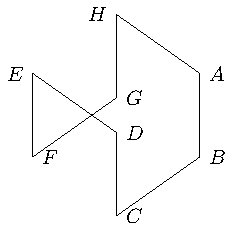
\includegraphics[width=0.75\linewidth]{202401311000-TikZ_files/figure-latex/unnamed-chunk-63-1} \caption{cube rotate}\label{fig:unnamed-chunk-63}
\end{figure}

\url{https://tex.stackexchange.com/questions/388621/optimizing-perspective-tikz-graphic}

\begin{figure}
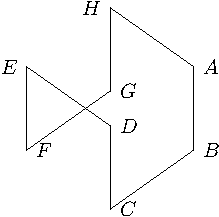
\includegraphics[width=0.75\linewidth]{202401311000-TikZ_files/figure-latex/unnamed-chunk-64-1} \caption{cube rotate}\label{fig:unnamed-chunk-64}
\end{figure}

\begin{figure}
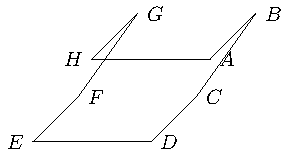
\includegraphics[width=0.75\linewidth]{202401311000-TikZ_files/figure-latex/unnamed-chunk-65-1} \caption{cube rotate}\label{fig:unnamed-chunk-65}
\end{figure}

\url{https://github.com/XiangyunHuang/bookdown-broken/blob/master/index.Rmd}

\begin{Shaded}
\begin{Highlighting}[]
\FunctionTok{\textbackslash{}smartdiagramset}\NormalTok{\{planet color=gray!40!white, uniform color list=gray!40!white for 10 items\}}
\FunctionTok{\textbackslash{}smartdiagram}\NormalTok{[bubble diagram]\{Basic skills,}
\NormalTok{  Edit\textasciitilde{}/}\FunctionTok{\textbackslash{}\textbackslash{}}\NormalTok{ (RStudio), Organize\textasciitilde{}/}\FunctionTok{\textbackslash{}\textbackslash{}}\NormalTok{ (bookdown), Cooperate\textasciitilde{}/}\FunctionTok{\textbackslash{}\textbackslash{}}\NormalTok{ (Git), Typeset\textasciitilde{}/}\FunctionTok{\textbackslash{}\textbackslash{}}\NormalTok{ (LaTeX/Pandoc), Compile\textasciitilde{}/}\FunctionTok{\textbackslash{}\textbackslash{}}\NormalTok{ (GitHub Action)\}}
\end{Highlighting}
\end{Shaded}

\begin{figure}
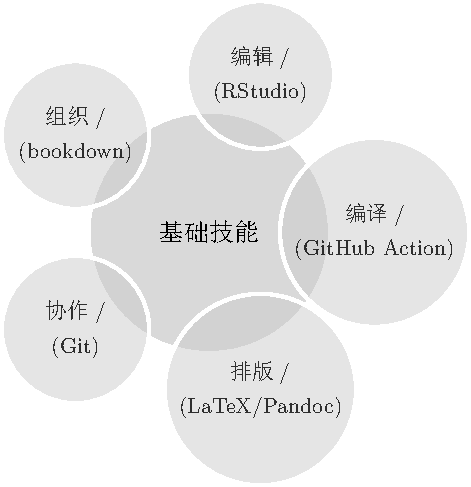
\includegraphics[width=0.65\linewidth]{202401311000-TikZ_files/figure-latex/skills-1} \caption{modern statistics plot skills}\label{fig:skills}
\end{figure}

\hypertarget{animation}{%
\section{animation}\label{animation}}

\url{https://zhuanlan.zhihu.com/p/338402487}

\hypertarget{xy-pic}{%
\chapter{xy-pic}\label{xy-pic}}

\url{https://bookdown.org/yihui/rmarkdown-cookbook/install-latex-pkgs.html}

\texttt{tinytex::install\_tinytex()}

the following xymatrix from LaTeX package xy for xy-pic is not shown or rendered in HTML:

\texttt{\$\textbackslash{}LaTeX\$} can only be used in HTML, not PDF

\xymatrix{U\ar[ddr]_{\psi}\ar[drr]^{\varphi}\ar[dr]|-{(x,y)}\\
 & X\times_{Z}Y\ar[d]^{q}\ar[r]_{p} & X\ar[d]_{f}\\
 & Y\ar[r]^{g} & Z
}

\hypertarget{statistics}{%
\chapter{statistics}\label{statistics}}

\hypertarget{covariance-matrix}{%
\section{covariance matrix}\label{covariance-matrix}}

\textsuperscript{\protect\hyperlink{ref-ccjou2014}{5}}

\hypertarget{calculation}{%
\subsection{calculation}\label{calculation}}

\begin{align*}
\mathrm{C}\left[\boldsymbol{X}\right]=\mathrm{Cov}\left[\boldsymbol{X}\right]=\mathrm{V}\left[\boldsymbol{X}\right]= & \mathrm{E}\left[\left[\boldsymbol{X}-\mathrm{E}\left(\boldsymbol{X}\right)\right]\left[\boldsymbol{X}-\mathrm{E}\left(\boldsymbol{X}\right)\right]^{\mathrm{T}}\right]\\
= & \mathrm{E}\left[\left[\boldsymbol{X}-\mathrm{E}\left(\boldsymbol{X}\right)\right]\left[\boldsymbol{X}^{\mathrm{T}}-\mathrm{E}\left(\boldsymbol{X}\right)^{\mathrm{T}}\right]\right]\\
= & \mathrm{E}\left[\boldsymbol{X}\boldsymbol{X}^{\mathrm{T}}-\mathrm{E}\left(\boldsymbol{X}\right)\boldsymbol{X}^{\mathrm{T}}-\boldsymbol{X}\mathrm{E}\left(\boldsymbol{X}\right)^{\mathrm{T}}+\mathrm{E}\left(\boldsymbol{X}\right)\mathrm{E}\left(\boldsymbol{X}\right)^{\mathrm{T}}\right]\\
= & \mathrm{E}\left[\boldsymbol{X}\boldsymbol{X}^{\mathrm{T}}\right]-\mathrm{E}\left[\mathrm{E}\left(\boldsymbol{X}\right)\boldsymbol{X}^{\mathrm{T}}\right]-\mathrm{E}\left[\boldsymbol{X}\mathrm{E}\left(\boldsymbol{X}\right)^{\mathrm{T}}\right]+\mathrm{E}\left[\mathrm{E}\left(\boldsymbol{X}\right)\mathrm{E}\left(\boldsymbol{X}\right)^{\mathrm{T}}\right]\\
= & \mathrm{E}\left[\boldsymbol{X}\boldsymbol{X}^{\mathrm{T}}\right]-\mathrm{E}\left(\boldsymbol{X}\right)\mathrm{E}\left[\boldsymbol{X}^{\mathrm{T}}\right]-\mathrm{E}\left[\boldsymbol{X}\right]\mathrm{E}\left(\boldsymbol{X}\right)^{\mathrm{T}}+\mathrm{E}\left(\boldsymbol{X}\right)\mathrm{E}\left(\boldsymbol{X}\right)^{\mathrm{T}}\\
= & \mathrm{E}\left[\boldsymbol{X}\boldsymbol{X}^{\mathrm{T}}\right]-\mathrm{E}\left(\boldsymbol{X}\right)\mathrm{E}\left(\boldsymbol{X}\right)^{\mathrm{T}}-\mathrm{E}\left(\boldsymbol{X}\right)\mathrm{E}\left(\boldsymbol{X}\right)^{\mathrm{T}}+\mathrm{E}\left(\boldsymbol{X}\right)\mathrm{E}\left(\boldsymbol{X}\right)^{\mathrm{T}}\\
= & \mathrm{E}\left[\boldsymbol{X}\boldsymbol{X}^{\mathrm{T}}\right]-\mathrm{E}\left(\boldsymbol{X}\right)\mathrm{E}\left(\boldsymbol{X}\right)^{\mathrm{T}}
\end{align*}

\begin{align*}
\boldsymbol{X}=\left[X\right]_{1\times1}=X\Rightarrow C\left(X\right)=\mathrm{C}\left[\boldsymbol{X}\right]= & \mathrm{E}\left[\boldsymbol{X}\boldsymbol{X}^{\mathrm{T}}\right]-\mathrm{E}\left(\boldsymbol{X}\right)\mathrm{E}\left(\boldsymbol{X}\right)^{\mathrm{T}}\\
= & \mathrm{E}\left[XX\right]-\mathrm{E}\left(X\right)\mathrm{E}\left(X\right)\\
= & \mathrm{E}\left(X^{2}\right)-\left[\mathrm{E}\left(X\right)\right]^{2}=\mathrm{V}\left(X\right)
\end{align*}

\hypertarget{mathrmvleftboldsymbolxboldsymbolbrightmathrmvleftboldsymbolxright}{%
\subsection{\texorpdfstring{\(\mathrm{V}\left[\boldsymbol{X}+\boldsymbol{b}\right]=\mathrm{V}\left[\boldsymbol{X}\right]\)}{\textbackslash mathrm\{V\}\textbackslash left{[}\textbackslash boldsymbol\{X\}+\textbackslash boldsymbol\{b\}\textbackslash right{]}=\textbackslash mathrm\{V\}\textbackslash left{[}\textbackslash boldsymbol\{X\}\textbackslash right{]}}}\label{mathrmvleftboldsymbolxboldsymbolbrightmathrmvleftboldsymbolxright}}

\begin{align*}
\mathrm{V}\left[\boldsymbol{X}+\boldsymbol{b}\right]= & \mathrm{E}\left[\left[\left(\boldsymbol{X}+\boldsymbol{b}\right)-\mathrm{E}\left(\boldsymbol{X}+\boldsymbol{b}\right)\right]\left[\left(\boldsymbol{X}+\boldsymbol{b}\right)-\mathrm{E}\left(\boldsymbol{X}+\boldsymbol{b}\right)\right]^{\mathrm{T}}\right]\\
\overset{\mathrm{E}\left(\boldsymbol{X}+\boldsymbol{b}\right)=\mathrm{E}\left(\boldsymbol{X}\right)+\boldsymbol{b}}{=} & \mathrm{E}\left[\left[\boldsymbol{X}+\boldsymbol{b}-\mathrm{E}\left(\boldsymbol{X}\right)-\boldsymbol{b}\right]\left[\boldsymbol{X}+\boldsymbol{b}-\mathrm{E}\left(\boldsymbol{X}\right)-\boldsymbol{b}\right]^{\mathrm{T}}\right]\\
= & \mathrm{E}\left[\left[\boldsymbol{X}-\mathrm{E}\left(\boldsymbol{X}\right)\right]\left[\boldsymbol{X}-\mathrm{E}\left(\boldsymbol{X}\right)\right]^{\mathrm{T}}\right]=\mathrm{V}\left[\boldsymbol{X}\right]
\end{align*}

\hypertarget{mathrmvleftaboldsymbolxrightamathrmvleftboldsymbolxrightamathrmt}{%
\subsection{\texorpdfstring{\(\mathrm{V}\left[A\boldsymbol{X}\right]=A\mathrm{V}\left[\boldsymbol{X}\right]A^{\mathrm{T}}\)}{\textbackslash mathrm\{V\}\textbackslash left{[}A\textbackslash boldsymbol\{X\}\textbackslash right{]}=A\textbackslash mathrm\{V\}\textbackslash left{[}\textbackslash boldsymbol\{X\}\textbackslash right{]}A\^{}\{\textbackslash mathrm\{T\}\}}}\label{mathrmvleftaboldsymbolxrightamathrmvleftboldsymbolxrightamathrmt}}

\begin{align*}
\mathrm{V}\left[A\boldsymbol{X}\right]= & \mathrm{E}\left[\left[\left(A\boldsymbol{X}\right)-\mathrm{E}\left(A\boldsymbol{X}\right)\right]\left[\left(A\boldsymbol{X}\right)-\mathrm{E}\left(A\boldsymbol{X}\right)\right]^{\mathrm{T}}\right]\\
\overset{\mathrm{E}\left(A\boldsymbol{X}\right)=A\mathrm{E}\left(\boldsymbol{X}\right)}{=} & \mathrm{E}\left[\left[A\boldsymbol{X}-A\mathrm{E}\left(\boldsymbol{X}\right)\right]\left[A\boldsymbol{X}-A\mathrm{E}\left(\boldsymbol{X}\right)\right]^{\mathrm{T}}\right]\\
= & \mathrm{E}\left[A\left[\boldsymbol{X}-\mathrm{E}\left(\boldsymbol{X}\right)\right]\left[A\left[\boldsymbol{X}-\mathrm{E}\left(\boldsymbol{X}\right)\right]\right]^{\mathrm{T}}\right]\\
= & \mathrm{E}\left[A\left[\boldsymbol{X}-\mathrm{E}\left(\boldsymbol{X}\right)\right]\left[\boldsymbol{X}-\mathrm{E}\left(\boldsymbol{X}\right)\right]^{\mathrm{T}}A^{\mathrm{T}}\right]\\
= & A\mathrm{E}\left[\left[\boldsymbol{X}-\mathrm{E}\left(\boldsymbol{X}\right)\right]\left[\boldsymbol{X}-\mathrm{E}\left(\boldsymbol{X}\right)\right]^{\mathrm{T}}\right]A^{\mathrm{T}}=A\mathrm{V}\left[\boldsymbol{X}\right]A^{\mathrm{T}}
\end{align*}

\hypertarget{mathrmvleftaboldsymbolxboldsymbolbrightamathrmvleftboldsymbolxrightamathrmt}{%
\subsection{\texorpdfstring{\(\mathrm{V}\left[A\boldsymbol{X}+\boldsymbol{b}\right]=A\mathrm{V}\left[\boldsymbol{X}\right]A^{\mathrm{T}}\)}{\textbackslash mathrm\{V\}\textbackslash left{[}A\textbackslash boldsymbol\{X\}+\textbackslash boldsymbol\{b\}\textbackslash right{]}=A\textbackslash mathrm\{V\}\textbackslash left{[}\textbackslash boldsymbol\{X\}\textbackslash right{]}A\^{}\{\textbackslash mathrm\{T\}\}}}\label{mathrmvleftaboldsymbolxboldsymbolbrightamathrmvleftboldsymbolxrightamathrmt}}

\[
\mathrm{V}\left[A\boldsymbol{X}+\boldsymbol{b}\right]=\mathrm{V}\left[A\boldsymbol{X}\right]=A\mathrm{V}\left[\boldsymbol{X}\right]A^{\mathrm{T}}
\]

\hypertarget{gosper-algorithm}{%
\chapter{Gosper algorithm}\label{gosper-algorithm}}

\hypertarget{lorentz-transformation}{%
\chapter{Lorentz transformation}\label{lorentz-transformation}}

\hypertarget{einstein}{%
\section{Einstein}\label{einstein}}

\url{https://wap.hillpublisher.com/UpFile/202204/20220414165340.pdf}

\hypertarget{bondi-k-calculus}{%
\section{\texorpdfstring{Bondi \(k\)-calculus}{Bondi k-calculus}}\label{bondi-k-calculus}}

\url{https://en.wikipedia.org/wiki/Bondi_k-calculus}

\hypertarget{wordline-in-minkowski-space}{%
\section{wordline in Minkowski space}\label{wordline-in-minkowski-space}}

\hypertarget{wick-rotation}{%
\subsection{Wick rotation}\label{wick-rotation}}

\url{https://ncatlab.org/nlab/show/Wick+rotation}

\hypertarget{osterwalder-schrader-reconstruction-theorem}{%
\subsubsection{Osterwalder-Schrader reconstruction theorem}\label{osterwalder-schrader-reconstruction-theorem}}

\url{https://ncatlab.org/nlab/show/Osterwalder-Schrader+theorem}

\hypertarget{r}{%
\chapter{R}\label{r}}

\url{https://bookdown.org/tonykuoyj/eloquentr/getting-started.html}

\hypertarget{laplace-transform}{%
\chapter{Laplace transform}\label{laplace-transform}}

\hypertarget{conic-section}{%
\chapter{conic section}\label{conic-section}}

\begin{CJK}{UTF8}{bsmi}
conic section 圓錐曲線 / 圓錐截痕
\end{CJK}

\url{https://en.wikipedia.org/wiki/Conic_section}

\url{https://tex.stackexchange.com/questions/222882/drawing-minimal-xy-axis}

\begin{figure}
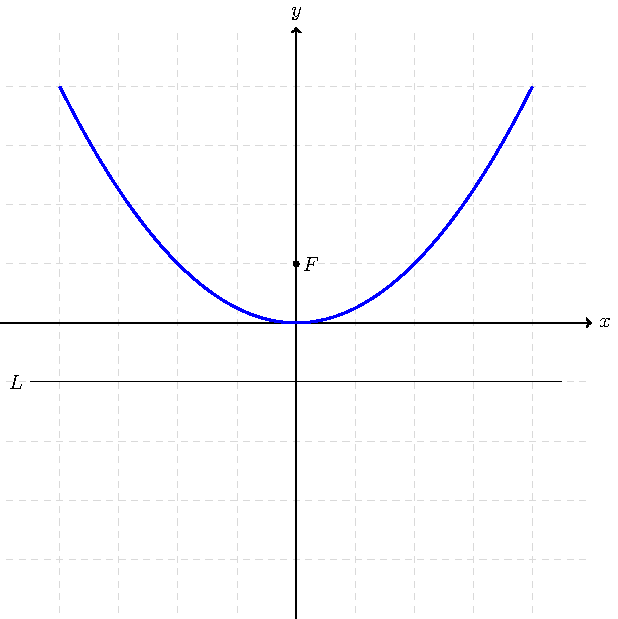
\includegraphics[width=0.75\linewidth]{202402252333-conic-section_files/figure-latex/unnamed-chunk-1-1} \caption{parabola defined by focus, directrix, eccentricity}\label{fig:unnamed-chunk-1}
\end{figure}

\hypertarget{cartesian-coordinate-focus-directrix-eccentricity}{%
\section{Cartesian coordinate: focus, directrix, eccentricity}\label{cartesian-coordinate-focus-directrix-eccentricity}}

\begin{CJK}{UTF8}{bsmi}
focus, directrix, eccentricity 焦點, 準線, 離心率
\end{CJK}

\[
\begin{cases}
F=\left(0,y_{{\scriptscriptstyle F}}\right) & F:\text{focus}\\
L=y-y_{{\scriptscriptstyle L}}=0 & L:\text{directrix}\\
\epsilon=\dfrac{\overline{PF}}{d\left(P,L\right)}=\dfrac{\left\Vert \left(x,y\right)-\left(0,y_{{\scriptscriptstyle F}}\right)\right\Vert }{\left\Vert y-y_{{\scriptscriptstyle L}}\right\Vert } & \begin{cases}
P=\left(x,y\right)\\
\epsilon:\text{eccentricity}
\end{cases}
\end{cases}
\]

\begin{align}
0\le\epsilon=\dfrac{\overline{PF}}{d\left(P,L\right)}=\dfrac{\overline{PF}}{\overline{PP^{\prime}}}= & \dfrac{\left\Vert \left(x,y\right)-\left(0,y_{{\scriptscriptstyle F}}\right)\right\Vert }{\left\Vert \left(x,y\right)-\left(x,y_{{\scriptscriptstyle L}}\right)\right\Vert }=\dfrac{\left\Vert \left(x,y-y_{{\scriptscriptstyle F}}\right)\right\Vert }{\left\Vert \left(0,y-y_{{\scriptscriptstyle L}}\right)\right\Vert }=\dfrac{\sqrt{x^{2}+\left(y-y_{{\scriptscriptstyle F}}\right)^{2}}}{\sqrt{\left(y-y_{{\scriptscriptstyle L}}\right)^{2}}} \label{eq:eccentricity}\\
\epsilon^{2}= & \dfrac{x^{2}+\left(y-y_{{\scriptscriptstyle F}}\right)^{2}}{\left(y-y_{{\scriptscriptstyle L}}\right)^{2}}=\dfrac{x^{2}+y^{2}-2y_{{\scriptscriptstyle F}}y+y_{{\scriptscriptstyle F}}^{2}}{y^{2}-2y_{{\scriptscriptstyle L}}y+y_{{\scriptscriptstyle L}}^{2}}\\
0= & x^{2}+\left(1-\epsilon^{2}\right)y^{2}-2\left(y_{{\scriptscriptstyle F}}-\epsilon^{2}y_{{\scriptscriptstyle L}}\right)y+\left(y_{{\scriptscriptstyle F}}^{2}-\epsilon^{2}y_{{\scriptscriptstyle L}}^{2}\right)\\
\overset{\epsilon\ne1}{=} & x^{2}+\left(1-\epsilon^{2}\right)\left[y^{2}-\dfrac{2\left(y_{{\scriptscriptstyle F}}-\epsilon^{2}y_{{\scriptscriptstyle L}}\right)}{1-\epsilon^{2}}y+\dfrac{y_{{\scriptscriptstyle F}}^{2}-\epsilon^{2}y_{{\scriptscriptstyle L}}^{2}}{1-\epsilon^{2}}\right]\\
= & x^{2}+\left(1-\epsilon^{2}\right)\\
 & \left[y^{2}-\dfrac{2\left(y_{{\scriptscriptstyle F}}-\epsilon^{2}y_{{\scriptscriptstyle L}}\right)}{1-\epsilon^{2}}y+\left(\dfrac{y_{{\scriptscriptstyle F}}-\epsilon^{2}y_{{\scriptscriptstyle L}}}{1-\epsilon^{2}}\right)^{2}-\left(\dfrac{y_{{\scriptscriptstyle F}}-\epsilon^{2}y_{{\scriptscriptstyle L}}}{1-\epsilon^{2}}\right)^{2}+\dfrac{y_{{\scriptscriptstyle F}}^{2}-\epsilon^{2}y_{{\scriptscriptstyle L}}^{2}}{1-\epsilon^{2}}\right]\\
= & x^{2}+\left(1-\epsilon^{2}\right)\left[\left(y-\dfrac{y_{{\scriptscriptstyle F}}-\epsilon^{2}y_{{\scriptscriptstyle L}}}{1-\epsilon^{2}}\right)^{2}+\dfrac{\left(y_{{\scriptscriptstyle F}}^{2}-\epsilon^{2}y_{{\scriptscriptstyle L}}^{2}\right)\left(1-\epsilon^{2}\right)-\left(y_{{\scriptscriptstyle F}}-\epsilon^{2}y_{{\scriptscriptstyle L}}\right)^{2}}{\left(1-\epsilon^{2}\right)^{2}}\right]\\
= & x^{2}+\left(1-\epsilon^{2}\right)\left(y-\dfrac{y_{{\scriptscriptstyle F}}-\epsilon^{2}y_{{\scriptscriptstyle L}}}{1-\epsilon^{2}}\right)^{2}+\dfrac{\colorbox{yellow!50}{\text{\ensuremath{\left(y_{{\scriptscriptstyle F}}^{2}-\epsilon^{2}y_{{\scriptscriptstyle L}}^{2}\right)\left(1-\epsilon^{2}\right)}-\ensuremath{\left(y_{{\scriptscriptstyle F}}-\epsilon^{2}y_{{\scriptscriptstyle L}}\right)^{2}}}}}{1-\epsilon^{2}}
\end{align}

\[
\begin{aligned}
 & \colorbox{yellow!50}{\text{\ensuremath{\left(y_{{\scriptscriptstyle F}}^{2}-\epsilon^{2}y_{{\scriptscriptstyle L}}^{2}\right)\left(1-\epsilon^{2}\right)}-\ensuremath{\left(y_{{\scriptscriptstyle F}}-\epsilon^{2}y_{{\scriptscriptstyle L}}\right)^{2}}}}\\
= & \left(1-\epsilon^{2}\right)y_{{\scriptscriptstyle F}}^{2}-\left(\epsilon^{2}-\epsilon^{4}\right)y_{{\scriptscriptstyle L}}^{2}-y_{{\scriptscriptstyle F}}^{2}+2\epsilon^{2}y_{{\scriptscriptstyle F}}y_{{\scriptscriptstyle L}}-\epsilon^{4}y_{{\scriptscriptstyle L}}^{2}\\
= & -\epsilon^{2}y_{{\scriptscriptstyle F}}^{2}-\epsilon^{2}y_{{\scriptscriptstyle L}}^{2}+2\epsilon^{2}y_{{\scriptscriptstyle F}}y_{{\scriptscriptstyle L}}=-\colorbox{red!50}{\text{\ensuremath{\epsilon^{2}\left(y_{{\scriptscriptstyle F}}-y_{{\scriptscriptstyle L}}\right)^{2}}}}
\end{aligned}
\]

\[
\begin{aligned}
\dfrac{\colorbox{red!50}{\text{\ensuremath{\epsilon^{2}\left(y_{{\scriptscriptstyle F}}-y_{{\scriptscriptstyle L}}\right)^{2}}}}}{1-\epsilon^{2}}\overset{\epsilon\ne1}{=} & x^{2}+\left(1-\epsilon^{2}\right)\left(y-\dfrac{y_{{\scriptscriptstyle F}}-\epsilon^{2}y_{{\scriptscriptstyle L}}}{1-\epsilon^{2}}\right)^{2}\\
1\overset{\epsilon\ne0,1}{=} & \begin{cases}
\left(\dfrac{x-0}{\dfrac{\epsilon\left(y_{{\scriptscriptstyle F}}-y_{{\scriptscriptstyle L}}\right)}{\sqrt{1-\epsilon^{2}}}}\right)^{2}+\left(\dfrac{y-\dfrac{y_{{\scriptscriptstyle F}}-\epsilon^{2}y_{{\scriptscriptstyle L}}}{1-\epsilon^{2}}}{\dfrac{\epsilon\left(y_{{\scriptscriptstyle F}}-y_{{\scriptscriptstyle L}}\right)}{1-\epsilon^{2}}}\right)^{2} & 1-\epsilon^{2}>0\overset{\epsilon\ge0}{\Rightarrow}0<\epsilon<1\\
-\left(\dfrac{x-0}{\dfrac{\epsilon\left(y_{{\scriptscriptstyle F}}-y_{{\scriptscriptstyle L}}\right)}{\sqrt{\epsilon^{2}-1}}}\right)^{2}+\left(\dfrac{y-\dfrac{y_{{\scriptscriptstyle F}}-\epsilon^{2}y_{{\scriptscriptstyle L}}}{1-\epsilon^{2}}}{\dfrac{\epsilon\left(y_{{\scriptscriptstyle F}}-y_{{\scriptscriptstyle L}}\right)}{1-\epsilon^{2}}}\right)^{2} & 1-\epsilon^{2}<0\overset{\epsilon\ge0}{\Rightarrow}\epsilon>1
\end{cases}
\end{aligned}
\]

\(\epsilon=0\) or \(\lim\limits _{\left|y_{L}\right|\rightarrow\infty}\epsilon=0\)

\[
r=\overline{PF}=\left\Vert \left(x,y\right)-\left(0,y_{{\scriptscriptstyle F}}\right)\right\Vert =\left\Vert \left(x,y-y_{{\scriptscriptstyle F}}\right)\right\Vert =\sqrt{x^{2}+\left(y-y_{{\scriptscriptstyle F}}\right)^{2}}
\]

\[
\epsilon=\dfrac{r}{d\left(P,L\right)}=\dfrac{\overline{PF}}{\overline{PP^{\prime}}}=\dfrac{\left\Vert \left(x,y\right)-\left(0,y_{{\scriptscriptstyle F}}\right)\right\Vert }{\left\Vert \left(x,y\right)-\left(x,y_{{\scriptscriptstyle L}}\right)\right\Vert }=\dfrac{\left\Vert \left(x,y-y_{{\scriptscriptstyle F}}\right)\right\Vert }{\left\Vert \left(0,y-y_{{\scriptscriptstyle L}}\right)\right\Vert }=\dfrac{\sqrt{x^{2}+\left(y-y_{{\scriptscriptstyle F}}\right)^{2}}}{\left|y-y_{{\scriptscriptstyle L}}\right|}
\]

\[
\lim_{\left|y_{L}\right|\rightarrow\infty}\epsilon=\lim_{\left|y_{L}\right|\rightarrow\infty}\dfrac{r}{d\left(P,L\right)}=\lim_{\left|y_{L}\right|\rightarrow\infty}\dfrac{\sqrt{x^{2}+\left(y-y_{{\scriptscriptstyle F}}\right)^{2}}}{\left|y-y_{{\scriptscriptstyle L}}\right|}=0
\]

\(\epsilon=1\)

\[
\begin{aligned}
0= & x^{2}+\left(1-\epsilon^{2}\right)y^{2}-2\left(y_{{\scriptscriptstyle F}}-\epsilon^{2}y_{{\scriptscriptstyle L}}\right)y+\left(y_{{\scriptscriptstyle F}}^{2}-\epsilon^{2}y_{{\scriptscriptstyle L}}^{2}\right)\\
\overset{\epsilon=1}{=} & x^{2}+\left(1-1^{2}\right)y^{2}-2\left(y_{{\scriptscriptstyle F}}-1^{2}y_{{\scriptscriptstyle L}}\right)y+\left(y_{{\scriptscriptstyle F}}^{2}-1^{2}y_{{\scriptscriptstyle L}}^{2}\right)\\
= & x^{2}-2\left(y_{{\scriptscriptstyle F}}-y_{{\scriptscriptstyle L}}\right)y+\left(y_{{\scriptscriptstyle F}}^{2}-y_{{\scriptscriptstyle L}}^{2}\right)\\
= & x^{2}-2\left(y_{{\scriptscriptstyle F}}-y_{{\scriptscriptstyle L}}\right)y+\left(y_{{\scriptscriptstyle F}}+y_{{\scriptscriptstyle L}}\right)\left(y_{{\scriptscriptstyle F}}-y_{{\scriptscriptstyle L}}\right)\\
x^{2}= & 2\left(y_{{\scriptscriptstyle F}}-y_{{\scriptscriptstyle L}}\right)\left(y-\dfrac{y_{{\scriptscriptstyle F}}+y_{{\scriptscriptstyle L}}}{2}\right)
\end{aligned}
\]

Let one curve vertex \(P=V=\left(0,0\right)\) on the curve, and fix the directrix \(L\) or \(y_{{\scriptscriptstyle L}}\),

\(\epsilon\ne1\)
\[
\begin{aligned}
 & 1\overset{P\left(x,y\right)=V\left(0,0\right)}{=}0+\left(\dfrac{0-\dfrac{y_{{\scriptscriptstyle F}}-\epsilon^{2}y_{{\scriptscriptstyle L}}}{1-\epsilon^{2}}}{\dfrac{\epsilon\left(y_{{\scriptscriptstyle F}}-y_{{\scriptscriptstyle L}}\right)}{1-\epsilon^{2}}}\right)^{2}\\
\Rightarrow & y_{{\scriptscriptstyle F}}-\epsilon^{2}y_{{\scriptscriptstyle L}}=\pm\epsilon\left(y_{{\scriptscriptstyle F}}-y_{{\scriptscriptstyle L}}\right)\\
\Rightarrow & \begin{cases}
\left(1-\epsilon\right)y_{{\scriptscriptstyle F}}=\epsilon\left(\epsilon-1\right)y_{{\scriptscriptstyle L}} & +\\
\left(1+\epsilon\right)y_{{\scriptscriptstyle F}}=\epsilon\left(\epsilon+1\right)y_{{\scriptscriptstyle L}} & -
\end{cases}\\
\Rightarrow & y_{{\scriptscriptstyle F}}=\begin{cases}
-\epsilon y_{{\scriptscriptstyle L}} & +\\
\epsilon y_{{\scriptscriptstyle L}} & -
\end{cases}
\end{aligned}
\]

\(\epsilon=1\)
\[
\begin{aligned}
 & x^{2}=2\left(y_{{\scriptscriptstyle F}}-y_{{\scriptscriptstyle L}}\right)\left(y-\dfrac{y_{{\scriptscriptstyle F}}+y_{{\scriptscriptstyle L}}}{2}\right)\\
\overset{P\left(x,y\right)=V\left(0,0\right)}{\Rightarrow} & 0^{2}=2\left(y_{{\scriptscriptstyle F}}-y_{{\scriptscriptstyle L}}\right)\left(0-\dfrac{y_{{\scriptscriptstyle F}}+y_{{\scriptscriptstyle L}}}{2}\right)\\
\Rightarrow & 0=\left(y_{{\scriptscriptstyle F}}-y_{{\scriptscriptstyle L}}\right)\left(y_{{\scriptscriptstyle F}}+y_{{\scriptscriptstyle L}}\right)\\
\Rightarrow & y_{{\scriptscriptstyle F}}=\mp y_{{\scriptscriptstyle L}}
\end{aligned}
\]

or by definition of eccentricity \eqref{eq:eccentricity}

\[
\begin{aligned}
0\le\epsilon=\dfrac{\overline{PF}}{d\left(P,L\right)}=\dfrac{\overline{PF}}{\overline{PP^{\prime}}}= & \dfrac{\left\Vert \left(x,y\right)-\left(0,y_{{\scriptscriptstyle F}}\right)\right\Vert }{\left\Vert \left(x,y\right)-\left(x,y_{{\scriptscriptstyle L}}\right)\right\Vert }=\dfrac{\left\Vert \left(x,y-y_{{\scriptscriptstyle F}}\right)\right\Vert }{\left\Vert \left(0,y-y_{{\scriptscriptstyle L}}\right)\right\Vert }=\dfrac{\sqrt{x^{2}+\left(y-y_{{\scriptscriptstyle F}}\right)^{2}}}{\sqrt{\left(y-y_{{\scriptscriptstyle L}}\right)^{2}}}\\
 & \overset{P\left(x,y\right)=V\left(0,0\right)}{=}\dfrac{\sqrt{0^{2}+\left(0-y_{{\scriptscriptstyle F}}\right)^{2}}}{\sqrt{\left(0-y_{{\scriptscriptstyle L}}\right)^{2}}}=\sqrt{\left(\dfrac{y_{{\scriptscriptstyle F}}}{y_{{\scriptscriptstyle L}}}\right)^{2}}\\
\epsilon^{2}= & \left(\dfrac{y_{{\scriptscriptstyle F}}}{y_{{\scriptscriptstyle L}}}\right)^{2}\Rightarrow y_{{\scriptscriptstyle F}}=\mp\epsilon y_{{\scriptscriptstyle L}}
\end{aligned}
\]

actually,

\[
y_{{\scriptscriptstyle F}}=-\epsilon y_{{\scriptscriptstyle L}}
\]

\hypertarget{two-definition-equivalence-for-ellipse-and-hyperbola}{%
\section{two-definition equivalence for ellipse and hyperbola}\label{two-definition-equivalence-for-ellipse-and-hyperbola}}

\url{https://math.stackexchange.com/questions/1833973/prove-that-the-directrix-focus-and-focus-focus-definitions-are-equivalent}

\url{https://www.geogebra.org/calculator/zkppuxwp}

\begin{figure}
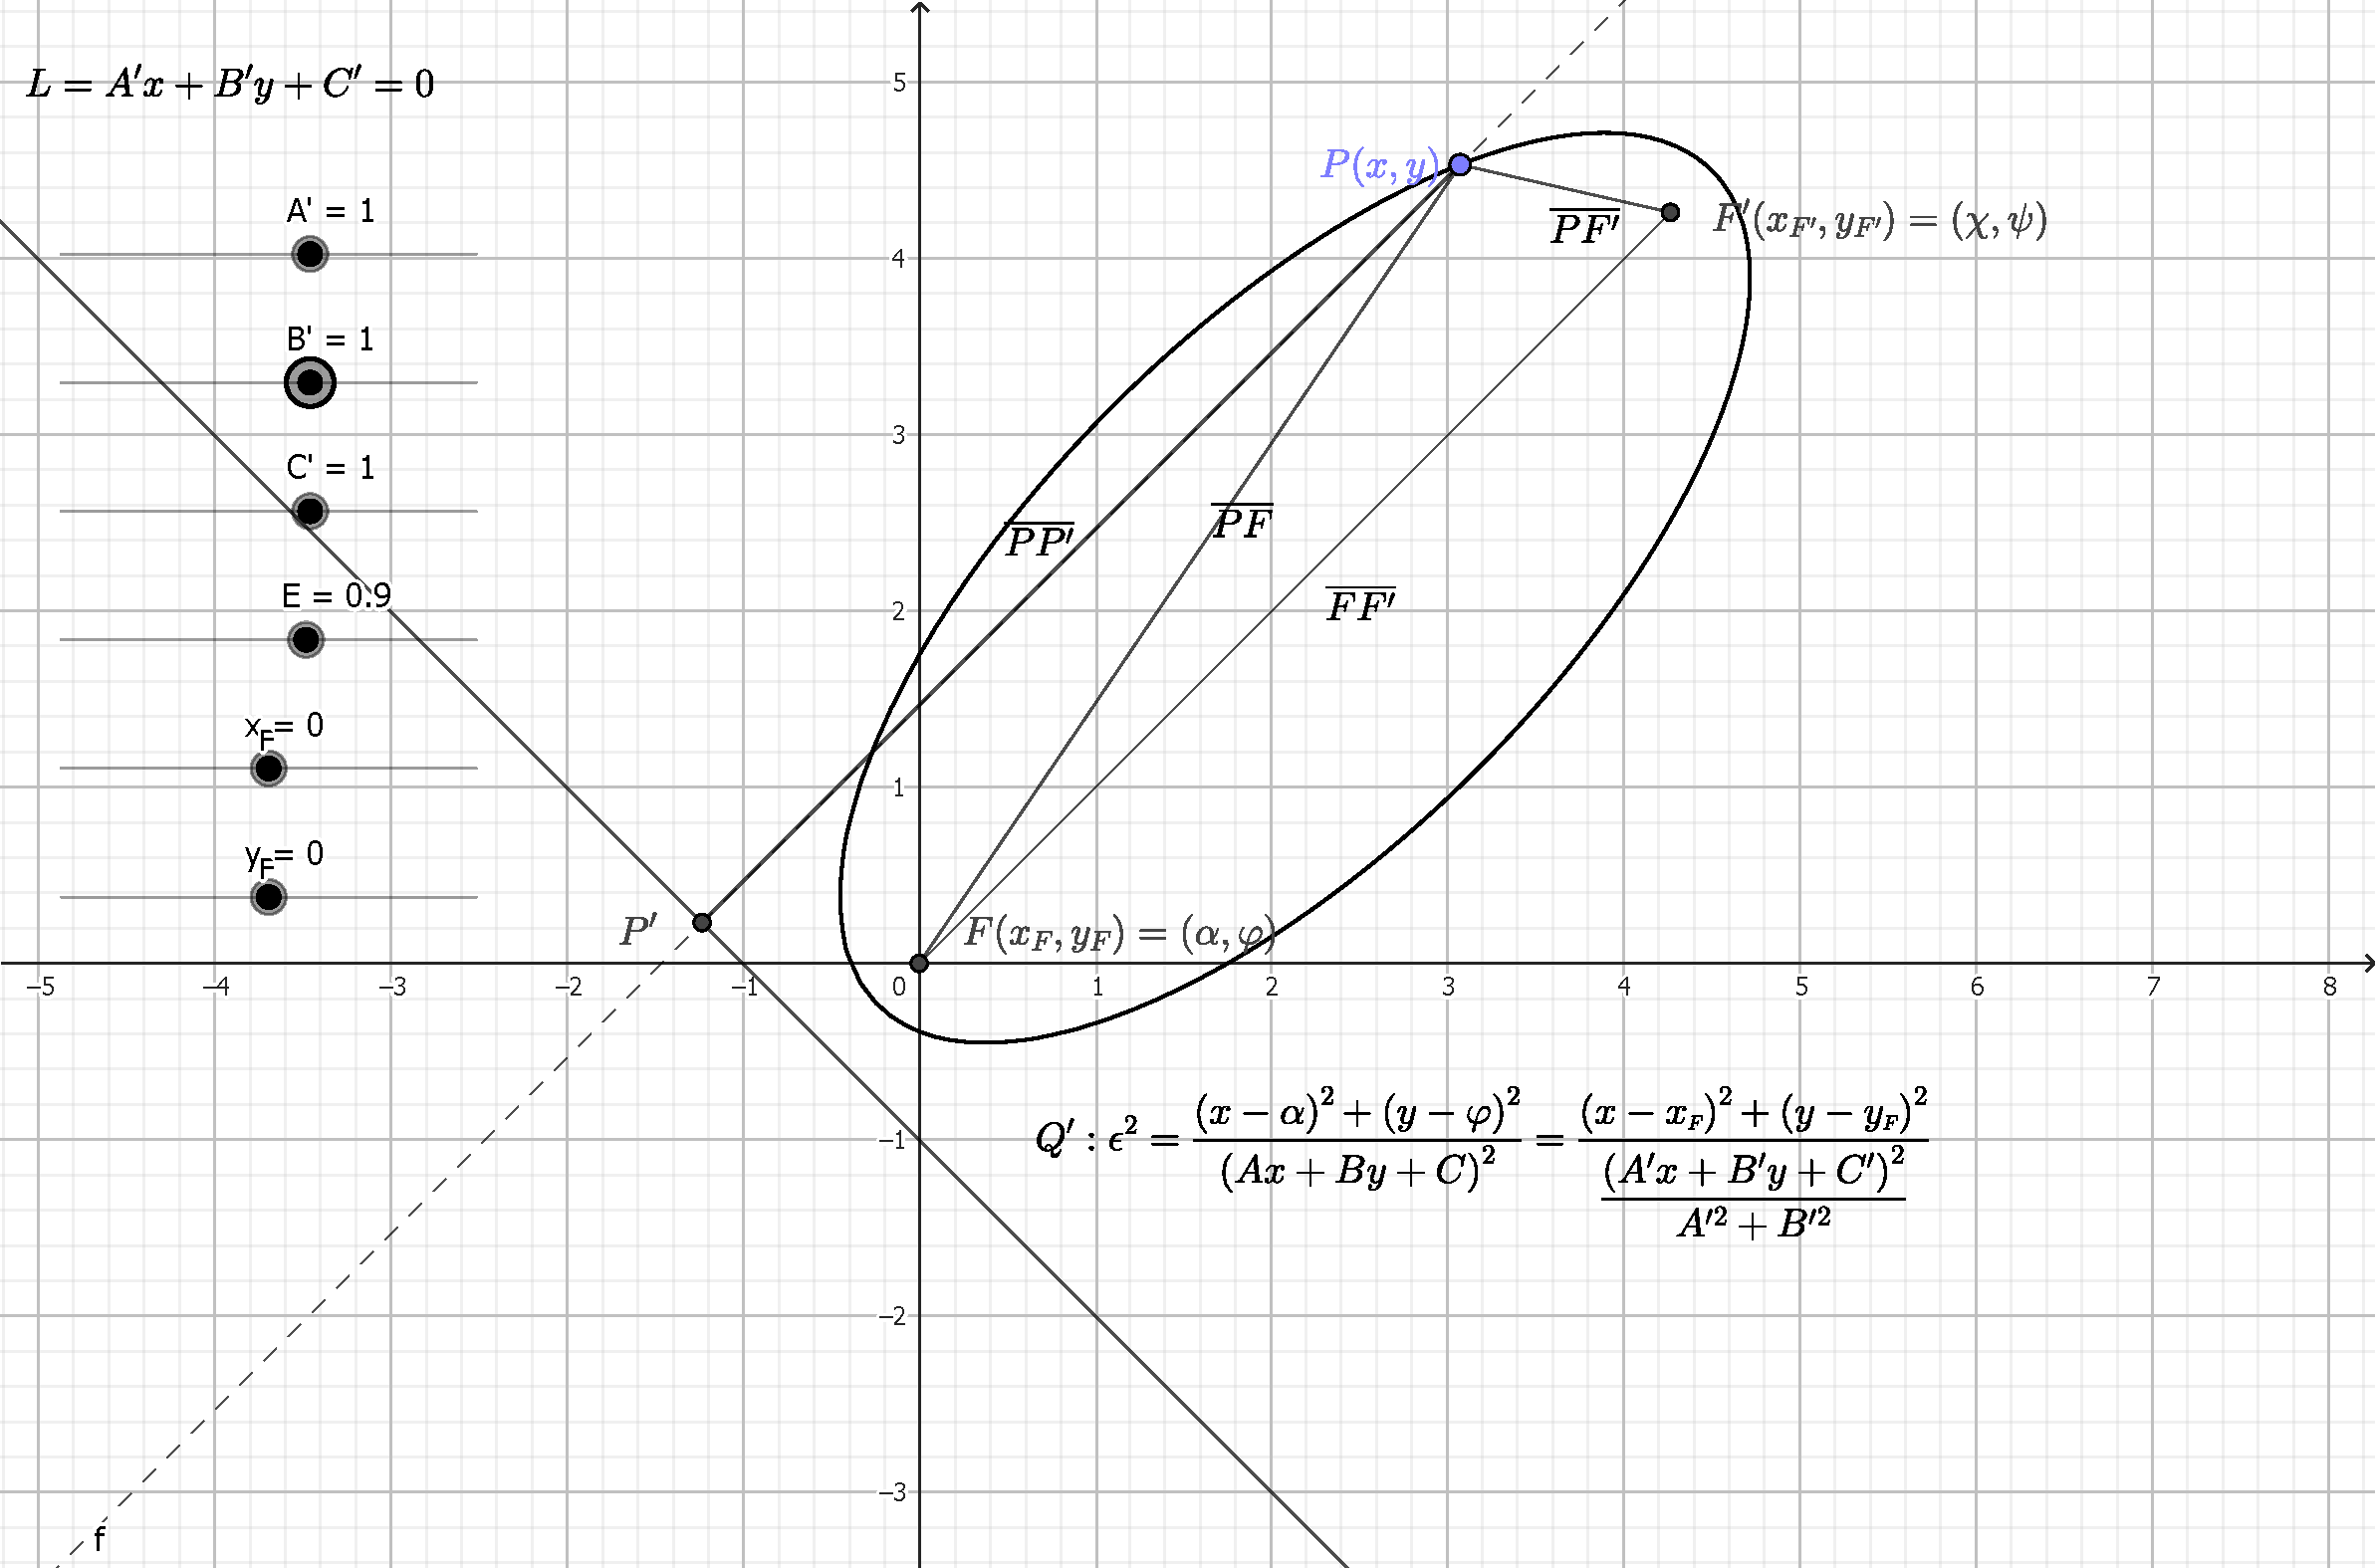
\includegraphics[width=0.75\linewidth]{img/conic-sections} \caption{conic sections}\label{fig:unnamed-chunk-3}
\end{figure}

\[
\begin{cases}
P=\left(x,y\right)\\
F=\left(x_{{\scriptscriptstyle F}},y_{{\scriptscriptstyle F}}\right)=\left(\alpha,\varphi\right) & F^{\prime}=\left(x_{{\scriptscriptstyle F^{\prime}}},y_{{\scriptscriptstyle F^{\prime}}}\right)=\left(\chi,\psi\right)\\
L=A^{\prime}x+B^{\prime}y+C^{\prime}=0
\end{cases}
\]

\hypertarget{first-definition-for-conic-sections-including-ellipses-and-hyperbolas}{%
\subsection{first definition for conic sections including ellipses and hyperbolas}\label{first-definition-for-conic-sections-including-ellipses-and-hyperbolas}}

\protect\hyperlink{distance-from-a-point-to-a-line}{distance from a point to a line}\textsuperscript{{[}\ref{distance-from-a-point-to-a-line}{]}}

\[
0\le\epsilon=\dfrac{\overline{PF}}{d\left(P,L\right)}=\dfrac{\sqrt{\left(x-x_{{\scriptscriptstyle F}}\right)^{2}+\left(y-y_{{\scriptscriptstyle F}}\right)^{2}}}{\dfrac{\left|A^{\prime}x+B^{\prime}y+C^{\prime}\right|}{\sqrt{A^{\prime}{}^{2}+B^{\prime}{}^{2}}}}=\dfrac{\sqrt{\left(x-\alpha\right)^{2}+\left(y-\varphi\right)^{2}}}{\left|Ax+By+C\right|},\begin{cases}
A=\dfrac{A^{\prime}}{\sqrt{A^{\prime}{}^{2}+B^{\prime}{}^{2}}}\\
B=\dfrac{B^{\prime}}{\sqrt{A^{\prime}{}^{2}+B^{\prime}{}^{2}}}\\
C=\dfrac{C^{\prime}}{\sqrt{A^{\prime}{}^{2}+B^{\prime}{}^{2}}}
\end{cases}
\]
\[
A^{2}+B^{2}=\left(\dfrac{A^{\prime}}{\sqrt{A^{\prime}{}^{2}+B^{\prime}{}^{2}}}\right)^{2}+\left(\dfrac{B^{\prime}}{\sqrt{A^{\prime}{}^{2}+B^{\prime}{}^{2}}}\right)^{2}=1
\]

or allowing \(\epsilon<0\) by squaring the definition

\[
\epsilon^{2}=\dfrac{\left(x-\alpha\right)^{2}+\left(y-\varphi\right)^{2}}{\left(Ax+By+C\right)^{2}}=\dfrac{\left(x-x_{{\scriptscriptstyle F}}\right)^{2}+\left(y-y_{{\scriptscriptstyle F}}\right)^{2}}{\dfrac{\left(A^{\prime}x+B^{\prime}y+C^{\prime}\right)^{2}}{A^{\prime}{}^{2}+B^{\prime}{}^{2}}}
\]

\[
\left(x-\alpha\right)^{2}+\left(y-\varphi\right)^{2}=\left[\epsilon\left(Ax+By+C\right)\right]^{2}
\]

\hypertarget{second-definition-for-ellipses-and-hyperbolas}{%
\subsection{second definition for ellipses and hyperbolas}\label{second-definition-for-ellipses-and-hyperbolas}}

\[
\begin{aligned}
2c=\overline{FF^{\prime}}= & \left\Vert \left(x_{{\scriptscriptstyle F}},y_{{\scriptscriptstyle F}}\right)-\left(x_{{\scriptscriptstyle F^{\prime}}},y_{{\scriptscriptstyle F^{\prime}}}\right)\right\Vert =\left\Vert \left(\alpha,\varphi\right)-\left(\chi,\psi\right)\right\Vert \\
= & \sqrt{\left(\alpha-\chi\right)^{2}+\left(\chi-\psi\right)^{2}}
\end{aligned}
\]

\[
\begin{aligned}
D= & \begin{cases}
\sqrt{\left(x-x_{{\scriptscriptstyle F}}\right)^{2}+\left(y-y_{{\scriptscriptstyle F}}\right)^{2}}+\sqrt{\left(x-x_{{\scriptscriptstyle F^{\prime}}}\right)^{2}+\left(y-y_{{\scriptscriptstyle F^{\prime}}}\right)^{2}} & \text{ellipse}\\
\sqrt{\left(x-x_{{\scriptscriptstyle F}}\right)^{2}+\left(y-y_{{\scriptscriptstyle F}}\right)^{2}}-\sqrt{\left(x-x_{{\scriptscriptstyle F^{\prime}}}\right)^{2}+\left(y-y_{{\scriptscriptstyle F^{\prime}}}\right)^{2}} & \text{hyperbola}
\end{cases}\\
= & \sqrt{\left(x-x_{{\scriptscriptstyle F}}\right)^{2}+\left(y-y_{{\scriptscriptstyle F}}\right)^{2}}\pm\sqrt{\left(x-x_{{\scriptscriptstyle F^{\prime}}}\right)^{2}+\left(y-y_{{\scriptscriptstyle F^{\prime}}}\right)^{2}}\\
= & \sqrt{\left(x-\alpha\right)^{2}+\left(y-\varphi\right)^{2}}\pm\sqrt{\left(x-\chi\right)^{2}+\left(y-\psi\right)^{2}}
\end{aligned}
\]

\[
\begin{aligned}
\left(x-\alpha\right)^{2}+\left(y-\varphi\right)^{2}= & \left(D\mp\sqrt{\left(x-\chi\right)^{2}+\left(y-\psi\right)^{2}}\right)^{2}\\
= & D^{2}\mp2D\sqrt{\left(x-\chi\right)^{2}+\left(y-\psi\right)^{2}}\\
 & +\left(x-\chi\right)^{2}+\left(y-\psi\right)^{2}
\end{aligned}
\]

\[
\begin{aligned}
D^{2}= & \left(x-\alpha\right)^{2}+\left(y-\varphi\right)^{2}+\left(x-\chi\right)^{2}+\left(y-\psi\right)^{2}\\
 & \pm2\sqrt{\left[\left(x-\alpha\right)^{2}+\left(y-\varphi\right)^{2}\right]\left[\left(x-\chi\right)^{2}+\left(y-\psi\right)^{2}\right]}\\
 & \left(x-\alpha\right)^{2}+\left(y-\varphi\right)^{2}+\left(x-\chi\right)^{2}+\left(y-\psi\right)^{2}-D^{2}\\
= & \mp2\sqrt{\left[\left(x-\alpha\right)^{2}+\left(y-\varphi\right)^{2}\right]\left[\left(x-\chi\right)^{2}+\left(y-\psi\right)^{2}\right]}\\
 & \left[\left(x-\alpha\right)^{2}+\left(y-\varphi\right)^{2}+\left(x-\chi\right)^{2}+\left(y-\psi\right)^{2}\right]^{2}+D^{4}\\
 & -2D^{2}\left[\left(x-\alpha\right)^{2}+\left(y-\varphi\right)^{2}+\left(x-\chi\right)^{2}+\left(y-\psi\right)^{2}\right]\\
= & 4\left[\left(x-\alpha\right)^{2}+\left(y-\varphi\right)^{2}\right]\left[\left(x-\chi\right)^{2}+\left(y-\psi\right)^{2}\right]\\
 & \left[\left(x-\alpha\right)^{2}+\left(y-\varphi\right)^{2}\right]^{2}+\left[\left(x-\chi\right)^{2}+\left(y-\psi\right)^{2}\right]^{2}\\
 & +2\left[\left(x-\alpha\right)^{2}+\left(y-\varphi\right)^{2}\right]\left[\left(x-\chi\right)^{2}+\left(y-\psi\right)^{2}\right]+D^{4}\\
 & -2D^{2}\left[\left(x-\alpha\right)^{2}+\left(y-\varphi\right)^{2}+\left(x-\chi\right)^{2}+\left(y-\psi\right)^{2}\right]\\
= & 4\left[\left(x-\alpha\right)^{2}+\left(y-\varphi\right)^{2}\right]\left[\left(x-\chi\right)^{2}+\left(y-\psi\right)^{2}\right]\\
0= & \left[\left(x-\alpha\right)^{2}+\left(y-\varphi\right)^{2}\right]^{2}+\left[\left(x-\chi\right)^{2}+\left(y-\psi\right)^{2}\right]^{2}\\
 & -2\left[\left(x-\alpha\right)^{2}+\left(y-\varphi\right)^{2}\right]\left[\left(x-\chi\right)^{2}+\left(y-\psi\right)^{2}\right]+D^{4}\\
 & -2D^{2}\left[\left(x-\alpha\right)^{2}+\left(y-\varphi\right)^{2}+\left(x-\chi\right)^{2}+\left(y-\psi\right)^{2}\right]\\
0= & \left\{ \left[\left(x-\alpha\right)^{2}+\left(y-\varphi\right)^{2}\right]-\left[\left(x-\chi\right)^{2}+\left(y-\psi\right)^{2}\right]\right\} ^{2}+D^{4}\\
 & -2D^{2}\left\{ \left[\left(x-\alpha\right)^{2}+\left(y-\varphi\right)^{2}\right]+\left[\left(x-\chi\right)^{2}+\left(y-\psi\right)^{2}\right]\right\} \\
0= & \left\{ \left[\left(x-\chi\right)^{2}+\left(y-\psi\right)^{2}\right]-\left[\left(x-\alpha\right)^{2}+\left(y-\varphi\right)^{2}\right]\right\} ^{2}+D^{4}\\
 & -2D^{2}\left\{ \left[\left(x-\chi\right)^{2}+\left(y-\psi\right)^{2}\right]-\left[\left(x-\alpha\right)^{2}+\left(y-\varphi\right)^{2}\right]\right\} \\
 & -4D^{2}\left[\left(x-\alpha\right)^{2}+\left(y-\varphi\right)^{2}\right]\\
 & \left(2D\right)^{2}\left[\left(x-\alpha\right)^{2}+\left(y-\varphi\right)^{2}\right]\\
= & \left\{ \left[\left(x-\chi\right)^{2}+\left(y-\psi\right)^{2}\right]-\left[\left(x-\alpha\right)^{2}+\left(y-\varphi\right)^{2}\right]-D^{2}\right\} ^{2}\\
= & \left\{ \left[\left(x-\chi\right)^{2}-\left(x-\alpha\right)^{2}\right]+\left[\left(y-\psi\right)^{2}-\left(y-\varphi\right)^{2}\right]-D^{2}\right\} ^{2}\\
= & \left\{ \left(2x-\chi-\alpha\right)\left(\alpha-\chi\right)+\left(2y-\psi-\varphi\right)\left(\varphi-\psi\right)-D^{2}\right\} ^{2}\\
= & \left\{ 2\left(\alpha-\chi\right)x-\left(\alpha^{2}-\chi^{2}\right)+2\left(\varphi-\psi\right)y-\left(\varphi^{2}-\psi^{2}\right)-D^{2}\right\} ^{2}\\
= & \left\{ 2\left(\alpha-\chi\right)x+2\left(\varphi-\psi\right)y-\left[\left(\alpha^{2}-\chi^{2}\right)+\left(\varphi^{2}-\psi^{2}\right)+D^{2}\right]\right\} ^{2}\\
D\ne0\\
 & \left(x-\alpha\right)^{2}+\left(y-\varphi\right)^{2}\\
= & \left[\dfrac{\alpha-\chi}{D}x+\dfrac{\varphi-\psi}{D}y-\left(\dfrac{\alpha^{2}-\chi^{2}}{2D}+\dfrac{\varphi^{2}-\psi^{2}}{2D}+\dfrac{D}{2}\right)\right]^{2}
\end{aligned}
\]

\[
\begin{cases}
\left(x-\alpha\right)^{2}+\left(y-\varphi\right)^{2}=\left[\epsilon\left(Ax+By+C\right)\right]^{2}\\
\left(x-\alpha\right)^{2}+\left(y-\varphi\right)^{2}=\left[\dfrac{\alpha-\chi}{D}x+\dfrac{\varphi-\psi}{D}y-\left(\dfrac{\alpha^{2}-\chi^{2}}{2D}+\dfrac{\varphi^{2}-\psi^{2}}{2D}+\dfrac{D}{2}\right)\right]^{2}
\end{cases}
\]

\[
\left(A,B,C\right)\rightleftarrows\left(\chi,\psi,D\right)
\]

\[
\begin{cases}
\epsilon A=\pm\dfrac{\alpha-\chi}{D} & \chi\pm\epsilon AD=\alpha\\
\epsilon B=\pm\dfrac{\varphi-\psi}{D} & \psi\pm\epsilon BD=\varphi\\
\epsilon C=\mp\left(\dfrac{\alpha^{2}-\chi^{2}}{2D}+\dfrac{\varphi^{2}-\psi^{2}}{2D}+\dfrac{D}{2}\right)
\end{cases}
\]

\[
\begin{aligned}
2\epsilon C= & \mp\left(\dfrac{\alpha-\chi}{D}\left(\alpha+\chi\right)+\dfrac{\varphi-\psi}{D}\left(\varphi+\psi\right)+D\right)\\
= & \mp\left(\pm\epsilon A\left(\alpha+\chi\right)\pm\epsilon B\left(\varphi+\psi\right)+D\right)\\
\mp\epsilon\left(A\alpha+B\varphi+2C\right)= & \pm\epsilon A\chi\pm\epsilon B\psi+D
\end{aligned}
\]

\[
\begin{pmatrix}1 & 0 & \pm\epsilon A\\
0 & 1 & \pm\epsilon B\\
\pm\epsilon A & \pm\epsilon B & 1
\end{pmatrix}\begin{pmatrix}\chi\\
\psi\\
D
\end{pmatrix}=\begin{pmatrix}\alpha\\
\varphi\\
\mp\epsilon\left(A\alpha+B\varphi+2C\right)
\end{pmatrix}
\]

\[
\begin{pmatrix}1 & 0 & \pm\epsilon A & \alpha\\
0 & 1 & \pm\epsilon B & \varphi\\
0 & \pm\epsilon B & 1\mp\epsilon^{2}A^{2} & \mp\epsilon\left(2A\alpha+B\varphi+2C\right)
\end{pmatrix}
\]

\[
\begin{pmatrix}1 & 0 & \pm\epsilon A & \alpha\\
0 & 1 & \pm\epsilon B & \varphi\\
0 & 0 & 1\mp\epsilon^{2}A^{2}\mp\epsilon^{2}B^{2} & \mp\epsilon\left(2A\alpha+2B\varphi+2C\right)
\end{pmatrix}
\]

\[
\begin{pmatrix}1 & 0 & \pm\epsilon A & \alpha\\
0 & 1 & \pm\epsilon B & \varphi\\
0 & 0 & 1 & \dfrac{\mp2\epsilon\left(A\alpha+B\varphi+C\right)}{1\mp\epsilon^{2}\left(A^{2}+B^{2}\right)}
\end{pmatrix}
\]

\[
A^{2}+B^{2}=\left(\dfrac{A^{\prime}}{\sqrt{A^{\prime}{}^{2}+B^{\prime}{}^{2}}}\right)^{2}+\left(\dfrac{B^{\prime}}{\sqrt{A^{\prime}{}^{2}+B^{\prime}{}^{2}}}\right)^{2}=1
\]

\[
\begin{cases}
\chi=\alpha\mp\epsilon AD=\alpha\mp\epsilon\dfrac{A^{\prime}}{\sqrt{A^{\prime}{}^{2}+B^{\prime}{}^{2}}}D\\
\psi=\varphi\mp\epsilon BD=\varphi\mp\epsilon\dfrac{B^{\prime}}{\sqrt{A^{\prime}{}^{2}+B^{\prime}{}^{2}}}D\\
D=\dfrac{\mp2\epsilon\left(A\alpha+B\varphi+C\right)}{1\mp\epsilon^{2}\left(A^{2}+B^{2}\right)}=\dfrac{\mp2\epsilon}{1\mp\epsilon^{2}}\dfrac{A^{\prime}\alpha+B^{\prime}\varphi+C^{\prime}}{\sqrt{A^{\prime}{}^{2}+B^{\prime}{}^{2}}} & A^{2}+B^{2}=1
\end{cases}
\]

actually, only one of two solutions is true

\[
\begin{cases}
\chi=\alpha-\epsilon AD=\alpha-\epsilon\dfrac{A^{\prime}}{\sqrt{A^{\prime}{}^{2}+B^{\prime}{}^{2}}}D=\alpha-\dfrac{2\epsilon^{2}}{\epsilon^{2}-1}\dfrac{A^{\prime}{}^{2}\alpha+A^{\prime}B^{\prime}\varphi+A^{\prime}C^{\prime}}{A^{\prime}{}^{2}+B^{\prime}{}^{2}}\\
\psi=\varphi-\epsilon BD=\varphi-\epsilon\dfrac{B^{\prime}}{\sqrt{A^{\prime}{}^{2}+B^{\prime}{}^{2}}}D=\varphi-\dfrac{2\epsilon^{2}}{\epsilon^{2}-1}\dfrac{A^{\prime}B^{\prime}\alpha+B^{\prime}{}^{2}\varphi+B^{\prime}C^{\prime}}{A^{\prime}{}^{2}+B^{\prime}{}^{2}}\\
D=\dfrac{-2\epsilon\left(A\alpha+B\varphi+C\right)}{1-\epsilon^{2}\left(A^{2}+B^{2}\right)}=\dfrac{-2\epsilon}{1-\epsilon^{2}}\dfrac{A^{\prime}\alpha+B^{\prime}\varphi+C^{\prime}}{\sqrt{A^{\prime}{}^{2}+B^{\prime}{}^{2}}}=\dfrac{2\epsilon}{\epsilon^{2}-1}\dfrac{A^{\prime}\alpha+B^{\prime}\varphi+C^{\prime}}{\sqrt{A^{\prime}{}^{2}+B^{\prime}{}^{2}}}
\end{cases}
\]

\[
\begin{cases}
\chi=\dfrac{\left(\epsilon^{2}-1\right)\left(A^{\prime}{}^{2}+B^{\prime}{}^{2}\right)\alpha-2\epsilon^{2}\left(A^{\prime}{}^{2}\alpha+A^{\prime}B^{\prime}\varphi+A^{\prime}C^{\prime}\right)}{\left(\epsilon^{2}-1\right)\left(A^{\prime}{}^{2}+B^{\prime}{}^{2}\right)}\\
\psi=\dfrac{\left(\epsilon^{2}-1\right)\left(A^{\prime}{}^{2}+B^{\prime}{}^{2}\right)\varphi-2\epsilon^{2}\left(A^{\prime}B^{\prime}\alpha+B^{\prime}{}^{2}\varphi+B^{\prime}C^{\prime}\right)}{\left(\epsilon^{2}-1\right)\left(A^{\prime}{}^{2}+B^{\prime}{}^{2}\right)}\\
\left|\dfrac{D}{d\left(F,L\right)}\right|=\left|\dfrac{2\epsilon}{1-\epsilon^{2}}\right|\Rightarrow\left(\dfrac{D}{d\left(F,L\right)}\right)^{2}=\left(\dfrac{2\epsilon}{1-\epsilon^{2}}\right)^{2}
\end{cases}
\]

\[
\begin{aligned}
 & \left(\epsilon^{2}-1\right)\left(A^{\prime}{}^{2}+B^{\prime}{}^{2}\right)\alpha-2\epsilon^{2}\left(A^{\prime}{}^{2}\alpha+A^{\prime}B^{\prime}\varphi+A^{\prime}C^{\prime}\right)\\
= & \left(-\left(\epsilon^{2}+1\right)A^{\prime}{}^{2}+\left(\epsilon^{2}-1\right)B^{\prime}{}^{2}\right)\alpha-2\epsilon^{2}\left(A^{\prime}B^{\prime}\varphi+A^{\prime}C^{\prime}\right)\\
= & \left(-\left(\epsilon^{2}+1\right)A^{\prime}{}^{2}+\left(\epsilon^{2}-1\right)B^{\prime}{}^{2}\right)\alpha-2\epsilon^{2}\left(A^{\prime}B^{\prime}\varphi+A^{\prime}C^{\prime}\right)
\end{aligned}
\]

Can the above be more simplified?

\[
\begin{aligned}
\overline{FF^{\prime}}^{2}= & \left(\alpha-\chi\right)^{2}+\left(\varphi-\psi\right)^{2}\\
= & \left(\alpha-\left(\alpha-\epsilon AD\right)\right)^{2}+\left(\varphi-\left(\varphi-\epsilon BD\right)\right)^{2}\\
= & \left(\epsilon D\right)^{2}\left(A^{2}+B^{2}\right)\\
= & \left(\epsilon D\right)^{2}
\end{aligned}
\]

\hypertarget{eccentricity-and-its-equivalent-representation}{%
\subsection{eccentricity and its equivalent representation}\label{eccentricity-and-its-equivalent-representation}}

\[
\left(\dfrac{c}{a}\right)^{2}=\left(\dfrac{\overline{PF}}{d\left(P,L\right)}\right)^{2}=\epsilon^{2}=\left(\dfrac{\overline{FF^{\prime}}}{D}\right)^{2}=\left(\dfrac{2c}{D}\right)^{2}\Rightarrow D=2a
\]

\[
\left(\dfrac{D}{d\left(F,L\right)}\right)^{2}=\left(\dfrac{2\epsilon}{1-\epsilon^{2}}\right)^{2}
\]

\begin{figure}
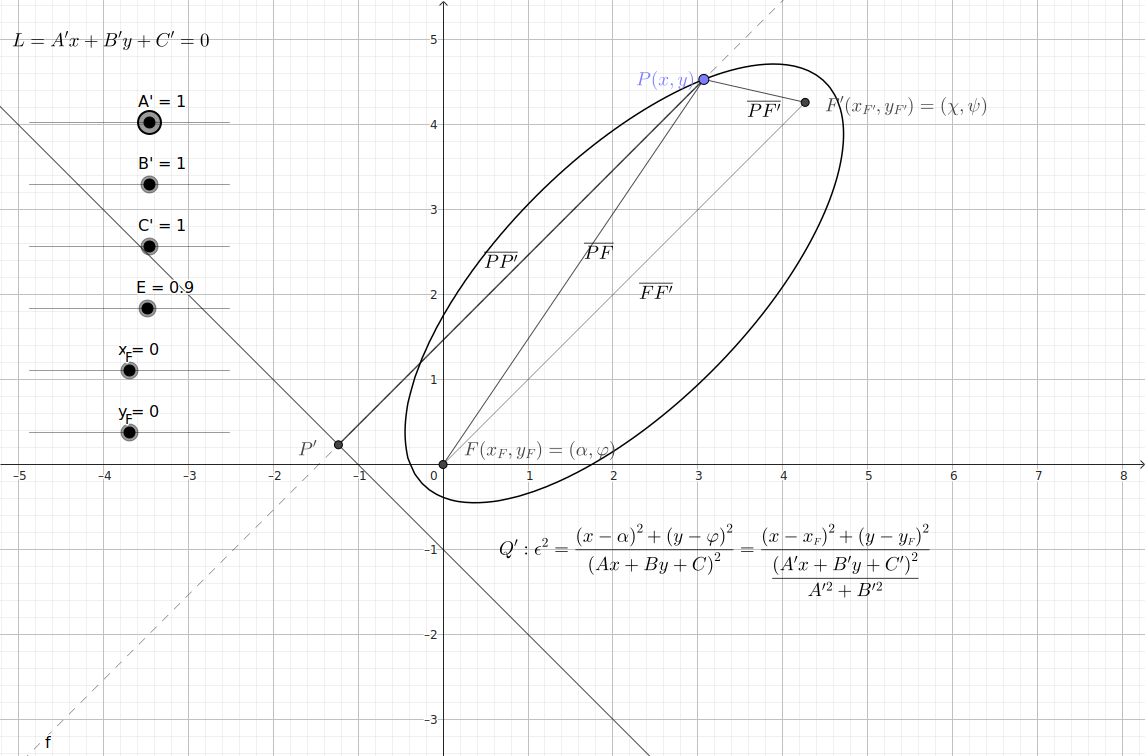
\includegraphics[width=0.75\linewidth]{img/conic-sections-ellipse} \caption{conic sections: ellipse}\label{fig:unnamed-chunk-4}
\end{figure}

\begin{figure}
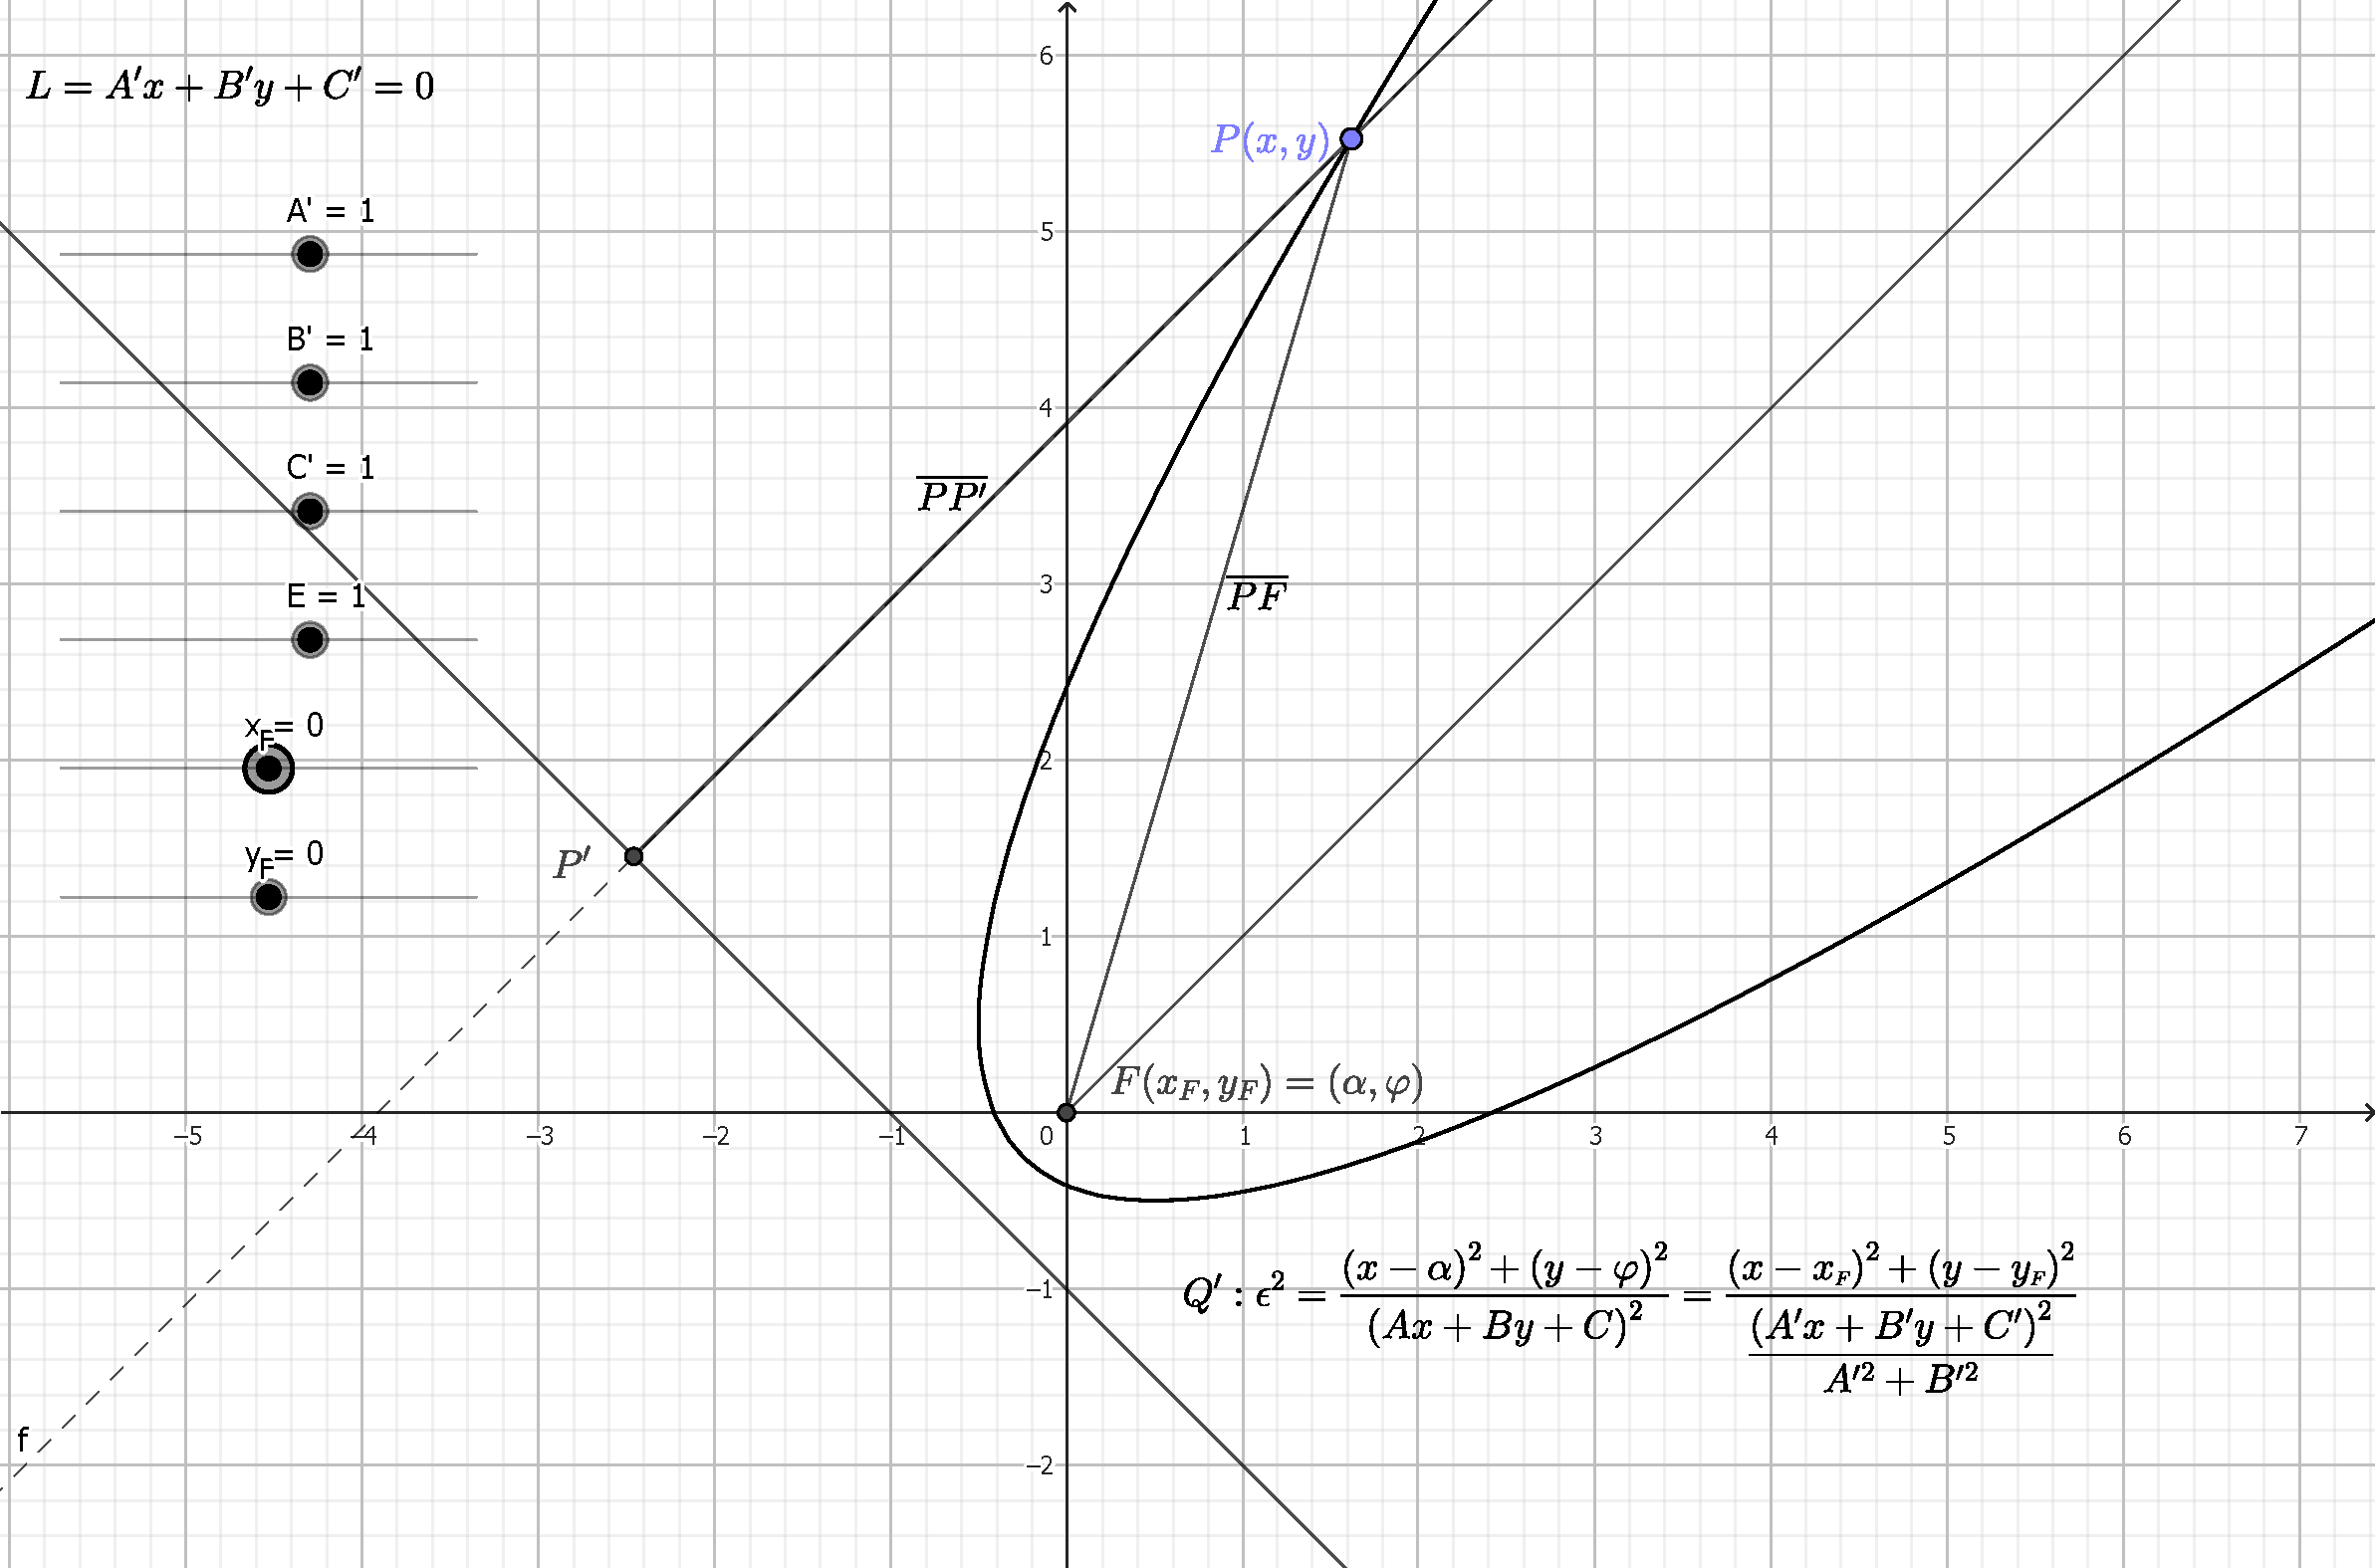
\includegraphics[width=0.75\linewidth]{img/conic-sections-parabola} \caption{conic sections: parabola}\label{fig:unnamed-chunk-5}
\end{figure}

\begin{figure}
\includegraphics[width=0.75\linewidth]{img/conic-sections-hyperbola} \caption{conic sections: hyperbola}\label{fig:unnamed-chunk-6}
\end{figure}

\hypertarget{cartesian-coordinate-standard-form-standard-equation}{%
\section{Cartesian coordinate: standard form / standard equation}\label{cartesian-coordinate-standard-form-standard-equation}}

\[
\begin{array}{ccccc}
\text{circle} & \left(\dfrac{y-k}{a}\right)^{2}+\left(\dfrac{x-h}{a}\right)^{2} & =1 &  & b=a\\
\text{ellipse} & \left(\dfrac{y-k}{b}\right)^{2}+\left(\dfrac{x-h}{a}\right)^{2} & =1 & \text{vertical} & b>a\\
 & \left(\dfrac{y-k}{b}\right)^{2}+\left(\dfrac{x-h}{a}\right)^{2} & =1 & \text{horizontal} & a>b\\
\text{parabola} & \left(y-k\right)-4c\left(x-h\right)^{2} & =0 & \text{vertical}\\
 & -4c\left(y-k\right)^{2}+\left(x-h\right) & =0 & \text{horizontal}\\
\text{hyperbola} & \left(\dfrac{y-k}{b}\right)^{2}-\left(\dfrac{x-h}{a}\right)^{2} & =1 & \text{vertical} & \dfrac{x-h}{a}=0\Rightarrow\dfrac{y-k}{b}=\pm1\\
 & -\left(\dfrac{y-k}{b}\right)^{2}+\left(\dfrac{x-h}{a}\right)^{2} & =1 & \text{horizontal} & \dfrac{y-k}{b}=0\Rightarrow\dfrac{x-h}{a}=\pm1
\end{array}
\]

\hypertarget{parametric-equation}{%
\section{parametric equation}\label{parametric-equation}}

\[
\begin{array}{cccccccc}
\text{circle} & \left(\dfrac{y-k}{a}\right)^{2}+\left(\dfrac{x-h}{a}\right)^{2} & =1 & \begin{pmatrix}x\\
y\\
1
\end{pmatrix}= & \begin{pmatrix}a & 0 & h\\
0 & a & k\\
0 & 0 & 1
\end{pmatrix} & \begin{pmatrix}\cos t\\
\sin t\\
1
\end{pmatrix} & =\begin{pmatrix}\cos t & 0 & h\\
0 & \sin t & k\\
0 & 0 & 1
\end{pmatrix} & \begin{pmatrix}a\\
a\\
1
\end{pmatrix}\\
\text{ellipse} & \left(\dfrac{y-k}{b}\right)^{2}+\left(\dfrac{x-h}{a}\right)^{2} & =1 & \begin{pmatrix}x\\
y\\
1
\end{pmatrix}= & \begin{pmatrix}a & 0 & h\\
0 & b & k\\
0 & 0 & 1
\end{pmatrix} & \begin{pmatrix}\cos t\\
\sin t\\
1
\end{pmatrix} & =\begin{pmatrix}\cos t & 0 & h\\
0 & \sin t & k\\
0 & 0 & 1
\end{pmatrix} & \begin{pmatrix}a\\
b\\
1
\end{pmatrix}\\
\text{parabola} & \left(y-k\right)-4c\left(x-h\right)^{2} & =0 & \begin{pmatrix}x\\
y\\
1
\end{pmatrix}= & \begin{pmatrix}1 & 0 & h\\
0 & 4c & k\\
0 & 0 & 1
\end{pmatrix} & \begin{pmatrix}t\\
t^{2}\\
1
\end{pmatrix} & =\begin{pmatrix}t & 0 & h\\
0 & t^{2} & k\\
0 & 0 & 1
\end{pmatrix} & \begin{pmatrix}1\\
4c\\
1
\end{pmatrix}\\
 & -4c\left(y-k\right)^{2}+\left(x-h\right) & =0 & \begin{pmatrix}x\\
y\\
1
\end{pmatrix}= & \begin{pmatrix}4c & 0 & h\\
0 & 1 & k\\
0 & 0 & 1
\end{pmatrix} & \begin{pmatrix}t^{2}\\
t\\
1
\end{pmatrix} & =\begin{pmatrix}t^{2} & 0 & h\\
0 & t & k\\
0 & 0 & 1
\end{pmatrix} & \begin{pmatrix}4c\\
1\\
1
\end{pmatrix}\\
\text{hyperbola} & \left(\dfrac{y-k}{b}\right)^{2}-\left(\dfrac{x-h}{a}\right)^{2} & =1 & \begin{pmatrix}x\\
y\\
1
\end{pmatrix}= & \begin{pmatrix}a & 0 & h\\
0 & b & k\\
0 & 0 & 1
\end{pmatrix} & \begin{pmatrix}\pm\cosh t\\
\sinh t\\
1
\end{pmatrix} & =\begin{pmatrix}\tan t & 0 & h\\
0 & \sec t & k\\
0 & 0 & 1
\end{pmatrix} & \begin{pmatrix}a\\
b\\
1
\end{pmatrix}\\
 & -\left(\dfrac{y-k}{b}\right)^{2}+\left(\dfrac{x-h}{a}\right)^{2} & =1 & \begin{pmatrix}x\\
y\\
1
\end{pmatrix}= & \begin{pmatrix}a & 0 & h\\
0 & b & k\\
0 & 0 & 1
\end{pmatrix} & \begin{pmatrix}\sinh t\\
\pm\cosh t\\
1
\end{pmatrix} & =\begin{pmatrix}\sec t & 0 & h\\
0 & \tan t & k\\
0 & 0 & 1
\end{pmatrix} & \begin{pmatrix}a\\
b\\
1
\end{pmatrix}
\end{array}
\]

\hypertarget{polar-coordinate}{%
\section{polar coordinate}\label{polar-coordinate}}

\[
\left(x-\alpha\right)^{2}+\left(y-\varphi\right)^{2}=\left[\epsilon\left(Ax+By+C\right)\right]^{2}
\]

\(\begin{cases}x=r\cos\theta\\y=r\sin\theta\end{cases}\)

\[
\left(r\cos\theta-\alpha\right)^{2}+\left(r\sin\theta-\varphi\right)^{2}=\left[\epsilon\left(Ar\cos\theta+Br\sin\theta+C\right)\right]^{2}
\]

If \(\begin{cases}F=\left(x_{{\scriptscriptstyle F}},y_{{\scriptscriptstyle F}}\right)=\left(\alpha,\varphi\right)=\left(0,0\right)\\L=Ax+By+C=x+p=0\end{cases}\)

\[
\begin{aligned}
\left(r\cos\theta\right)^{2}+\left(r\sin\theta\right)^{2}= & \left[\epsilon\left(r\cos\theta+p\right)\right]^{2}\\
r^{2}=\\
r= & \pm\epsilon\left(r\cos\theta+p\right)\\
= & \pm\left(r\epsilon\cos\theta+\epsilon p\right)\\
r\left(1\mp\epsilon\cos\theta\right)= & \epsilon p\\
r= & \dfrac{\epsilon p}{1\mp\epsilon\cos\theta}
\end{aligned}
\]

\url{https://www.geogebra.org/calculator/azksjxbq}

\(r=\dfrac{\epsilon p}{1-\epsilon\cos\theta}\) will not cross \(L=x+p=0\) on graphs, so maybe it is a more correct solution

\[
r=\dfrac{\epsilon p}{1-\epsilon\cos\theta}
\]

\begin{figure}
\includegraphics[width=0.75\linewidth]{img/conic-sections-polar-ellipse} \caption{polar conic sections: ellipse}\label{fig:unnamed-chunk-7}
\end{figure}

\begin{figure}
\includegraphics[width=0.75\linewidth]{img/conic-sections-polar-parabola} \caption{polar conic sections: parabola}\label{fig:unnamed-chunk-8}
\end{figure}

\begin{figure}
\includegraphics[width=0.75\linewidth]{img/conic-sections-polar-hyperbola} \caption{polar conic sections: hyperbola}\label{fig:unnamed-chunk-9}
\end{figure}

\url{https://ccjou.wordpress.com/2013/05/24/\%E5\%9C\%93\%E9\%8C\%90\%E6\%9B\%B2\%E7\%B7\%9A/}

\hypertarget{cartesian-coordinate-general-form-quadratic-equation}{%
\section{Cartesian coordinate: general form / quadratic equation}\label{cartesian-coordinate-general-form-quadratic-equation}}

\url{https://en.wikipedia.org/wiki/Matrix_representation_of_conic_sections}

\hypertarget{homogeneous-coordinate}{%
\section{homogeneous coordinate}\label{homogeneous-coordinate}}

\hypertarget{distance-from-a-point-to-a-line}{%
\chapter{distance from a point to a line}\label{distance-from-a-point-to-a-line}}

\begin{CJK}{UTF8}{bsmi}
點到直線距離
\end{CJK}

\begin{theorem}
\protect\hypertarget{thm:unnamed-chunk-1}{}\label{thm:unnamed-chunk-1}\[
\begin{array}{c}
\begin{cases}
P=P\left(x_{0},y_{0}\right)\\
L=L\left(x,y\right)=Ax+By+C=0,A^{2}+B^{2}\ne0
\end{cases}\\
\Downarrow\\
d\left(P,L\right)=\dfrac{\left|Ax_{0}+By_{0}+C\right|}{\sqrt{A^{2}+B^{2}}}
\end{array}
\]
\end{theorem}

\url{https://en.wikipedia.org/wiki/Distance_from_a_point_to_a_line}

\url{https://highscope.ch.ntu.edu.tw/wordpress/?p=47407}

\url{https://web.math.sinica.edu.tw/mathmedia/HTMLarticle18.jsp?mID=40312}

Proofs:

\hypertarget{by-shortest-overlineppprime}{%
\section{\texorpdfstring{by shortest \(\overline{PP^{\prime}}\)}{by shortest \textbackslash overline\{PP\^{}\{\textbackslash prime\}\}}}\label{by-shortest-overlineppprime}}

\[
\begin{aligned}
 & P^{\prime}=P^{\prime}\left(x,y\right)\in L=Ax+By+C=0\\
\Rightarrow & y=\dfrac{-1}{B}\left(Ax+C\right)
\end{aligned}
\]

\[
\begin{aligned}
\overline{PP^{\prime}}^{2}\left(x,y\right)= & \left(x_{0}-x\right)^{2}+\left(y_{0}-y\right)^{2}\\
= & \left(x_{0}-x\right)^{2}+\left(y_{0}-\dfrac{-1}{B}\left(Ax+C\right)\right)^{2}\\
= & \left(x-x_{0}\right)^{2}+\left(\dfrac{A}{B}x+\dfrac{C}{B}+y_{0}\right)^{2}=\overline{PP^{\prime}}^{2}\left(x\right)
\end{aligned}
\]

\[
\begin{aligned}
0=\dfrac{\partial}{\partial x}\overline{PP^{\prime}}^{2}\left(x\right)= & 2\left(x-x_{0}\right)+2\left(\dfrac{A}{B}x+\dfrac{C}{B}+y_{0}\right)\dfrac{A}{B}\\
= & \dfrac{2}{B^{2}}\left(B^{2}\left(x-x_{0}\right)+A^{2}x+AC+ABy_{0}\right)\\
= & \dfrac{2}{B^{2}}\left[\left(A^{2}+B^{2}\right)x-\left(B^{2}x_{0}-ABy_{0}-AC\right)\right]\\
x= & \dfrac{B^{2}x_{0}-ABy_{0}-AC}{A^{2}+B^{2}}
\end{aligned}
\]
or by completing the square to find \(x\)

\[
\begin{aligned}
 & \overline{PP^{\prime}}^{2}\left(x=\dfrac{B^{2}x_{0}-ABy_{0}-AC}{A^{2}+B^{2}}\right)\\
= & \left(\dfrac{B^{2}x_{0}-ABy_{0}-AC}{A^{2}+B^{2}}-x_{0}\right)^{2}+\left(\dfrac{A}{B}\dfrac{B^{2}x_{0}-ABy_{0}-AC}{A^{2}+B^{2}}+\dfrac{C}{B}+y_{0}\right)^{2}\\
= & \left(\dfrac{-A^{2}x_{0}-ABy_{0}-AC}{A^{2}+B^{2}}\right)^{2}+\left(\dfrac{A\left(B^{2}x_{0}-ABy_{0}-AC\right)+C\left(A^{2}+B^{2}\right)+B\left(A^{2}+B^{2}\right)y_{0}}{B\left(A^{2}+B^{2}\right)}\right)^{2}\\
= & \left(\dfrac{-A\left(Ax_{0}+By_{0}+C\right)}{A^{2}+B^{2}}\right)^{2}+\left(\dfrac{AB^{2}x_{0}+B^{3}y_{0}+B^{2}C}{B\left(A^{2}+B^{2}\right)}\right)^{2}\\
= & \dfrac{A^{2}\left(Ax_{0}+By_{0}+C\right)^{2}}{\left(A^{2}+B^{2}\right)^{2}}+\dfrac{B^{2}\left(Ax_{0}+By_{0}+C\right)^{2}}{\left(A^{2}+B^{2}\right)^{2}}\\
= & \dfrac{\left(Ax_{0}+By_{0}+C\right)^{2}}{A^{2}+B^{2}}\\
\overline{PP^{\prime}}= & \overline{PP^{\prime}}\left(x=\dfrac{B^{2}x_{0}-ABy_{0}-AC}{A^{2}+B^{2}}\right)=\dfrac{\left|Ax_{0}+By_{0}+C\right|}{\sqrt{A^{2}+B^{2}}}
\end{aligned}
\]

\hypertarget{by-perpendicular-foot}{%
\section{by perpendicular foot}\label{by-perpendicular-foot}}

\[
y=\dfrac{-A}{B}x-\dfrac{C}{B}=\dfrac{-1}{B}\left(Ax+C\right),\text{ if }B\ne0
\]

\[
L_{\perp}:\left(y=\dfrac{B}{A}x+K\right)\perp\left(y=\dfrac{-A}{B}x-\dfrac{C}{B}\right):L
\]

\[
L_{\perp}=L_{\perp}\left(x,y\right)=Bx-Ay+K=0
\]
\[
P=P\left(x_{0},y_{0}\right)\in L_{\perp}=B\left(x-x_{0}\right)-A\left(y-y_{0}\right)=0
\]

\[
L_{\perp}=Bx-Ay-\left(Bx_{0}-Ay_{0}\right)=0
\]
perpendicular foot = foot of the perpendicular \(P^{\prime}\)

\[
\begin{aligned}
P^{\prime}\in\left(L_{\perp}\cap L\right)= & \begin{cases}
L=Ax+By+C=0\\
L_{\perp}=Bx-Ay-\left(Bx_{0}-Ay_{0}\right)=0
\end{cases}\\
= & \begin{cases}
Ax+By=-C\\
Bx-Ay=Bx_{0}-Ay_{0}
\end{cases}\\
P^{\prime}=P^{\prime}\left(x,y\right)= & \left(\dfrac{\begin{vmatrix}-C & B\\
Bx_{0}-Ay_{0} & -A
\end{vmatrix}}{\begin{vmatrix}A & B\\
B & -A
\end{vmatrix}},\dfrac{\begin{vmatrix}A & -C\\
B & Bx_{0}-Ay_{0}
\end{vmatrix}}{\begin{vmatrix}A & B\\
B & -A
\end{vmatrix}}\right)\\
= & \left(\dfrac{\begin{vmatrix}C & B\\
-Bx_{0}+Ay_{0} & -A
\end{vmatrix}}{\begin{vmatrix}A & -B\\
B & A
\end{vmatrix}},\dfrac{\begin{vmatrix}A & C\\
B & -Bx_{0}+Ay_{0}
\end{vmatrix}}{\begin{vmatrix}A & -B\\
B & A
\end{vmatrix}}\right)\\
= & \left(\dfrac{B^{2}x_{0}-ABy_{0}-AC}{A^{2}+B^{2}},\dfrac{-ABx_{0}+A^{2}y_{0}-BC}{A^{2}+B^{2}}\right)
\end{aligned}
\]

\[
\begin{aligned}
 & d\left(P,L\right)=\overline{PP^{\prime}}\\
= & \left\Vert \left(x_{0},y_{0}\right)-\left(\dfrac{B^{2}x_{0}-ABy_{0}-AC}{A^{2}+B^{2}},\dfrac{-ABx_{0}+A^{2}y_{0}-BC}{A^{2}+B^{2}}\right)\right\Vert \\
= & \sqrt{\left(x_{0}-\dfrac{B^{2}x_{0}-ABy_{0}-AC}{A^{2}+B^{2}}\right)^{2}+\left(y_{0}-\dfrac{-ABx_{0}+A^{2}y_{0}-BC}{A^{2}+B^{2}}\right)^{2}}\\
= & \sqrt{\left(\dfrac{A^{2}x_{0}+ABy_{0}+AC}{A^{2}+B^{2}}\right)^{2}+\left(\dfrac{ABx_{0}+B^{2}y_{0}+BC}{A^{2}+B^{2}}\right)^{2}}\\
= & \sqrt{\dfrac{A^{2}\left(Ax_{0}+By_{0}+C\right)^{2}+B^{2}\left(Ax_{0}+By_{0}+C\right)^{2}}{\left(A^{2}+B^{2}\right)^{2}}}=\sqrt{\dfrac{\left(Ax_{0}+By_{0}+C\right)^{2}}{A^{2}+B^{2}}}\\
= & \dfrac{\left|Ax_{0}+By_{0}+C\right|}{\sqrt{A^{2}+B^{2}}}
\end{aligned}
\]

\hypertarget{by-normal-vector}{%
\section{by normal vector}\label{by-normal-vector}}

\[
\begin{cases}
\overset{\rightharpoonup}{n}=\left(A,B\right)\perp L=Ax+By+C=0\\
\overset{\rightharpoonup}{PP^{\prime}}=P^{\prime}-P=\left(x-x_{0},y-y_{0}\right)
\end{cases}
\]

\[
\begin{aligned}
 & \left|\overset{\rightharpoonup}{PP^{\prime}}\cdot\overset{\rightharpoonup}{n}\right|\\
= & \left\Vert \overset{\rightharpoonup}{PP^{\prime}}\right\Vert \left\Vert \overset{\rightharpoonup}{n}\right\Vert \left|\cos\theta\right|\\
\left\Vert \overset{\rightharpoonup}{PP^{\prime}}\right\Vert \left|\cos\theta\right|= & \left|\overset{\rightharpoonup}{PP^{\prime}}\cdot\widehat{\boldsymbol{n}}\right|\\
= & \dfrac{\left|\overset{\rightharpoonup}{PP^{\prime}}\cdot\overset{\rightharpoonup}{n}\right|}{\left\Vert \overset{\rightharpoonup}{n}\right\Vert }\\
= & \dfrac{\left|\left(x-x_{0},y-y_{0}\right)\cdot\left(A,B\right)\right|}{\left\Vert \left(A,B\right)\right\Vert }=\dfrac{\left|A\left(x-x_{0}\right)+B\left(y-y_{0}\right)\right|}{\sqrt{A^{2}+B^{2}}}\\
= & \dfrac{\left|-Ax_{0}-By_{0}+Ax+By\right|}{\sqrt{A^{2}+B^{2}}}\begin{subarray}{c}
Ax+By+C=0\\
=\\
Ax+By=-C
\end{subarray}\dfrac{\left|-Ax_{0}-By_{0}-C\right|}{\sqrt{A^{2}+B^{2}}}\\
= & \dfrac{\left|Ax_{0}+By_{0}+C\right|}{\sqrt{A^{2}+B^{2}}}
\end{aligned}
\]

PDF LaTeX \texttt{\textbackslash{}usepackage\{fdsymbol\}} to have \texttt{\textbackslash{}overrightharpoon} vector; however, there are too many side effects, including ugly mathptmx \(\sum\), \ldots{}

\begin{verbatim}
\usepackage{fdsymbol} % vector over accent, but will use mathptmx
% replace the rather ugly mathptmx \sum operator with the equivalent Computer Modern one
\let\sum\relax
\DeclareSymbolFont{CMlargesymbols}{OMX}{cmex}{m}{n}
\DeclareMathSymbol{\sum}{\mathop}{CMlargesymbols}{"50}
\end{verbatim}

\hypertarget{by-cauchy-inequality}{%
\section{by Cauchy inequality}\label{by-cauchy-inequality}}

\[
\begin{aligned}
Ax+By+C= & 0\\
Ax+By= & -C\\
\left(Ax+By\right)-\left(Ax_{0}+By_{0}\right)= & -C-\left(Ax_{0}+By_{0}\right)\\
A\left(x-x_{0}\right)+B\left(y-y_{0}\right)= & -\left(Ax_{0}+By_{0}+C\right)
\end{aligned}
\]

\[
\begin{aligned}
\overline{PP^{\prime}}^{2}= & \left(x_{0}-x\right)^{2}+\left(y_{0}-y\right)^{2}\\
\left[A^{2}+B^{2}\right]\overline{PP^{\prime}}^{2}= & \left[A^{2}+B^{2}\right]\left[\left(x_{0}-x\right)^{2}+\left(y_{0}-y\right)^{2}\right]\\
\ge & \left[A\left(x-x_{0}\right)+B\left(y-y_{0}\right)\right]^{2}\\
= & \left[-\left(Ax_{0}+By_{0}+C\right)\right]^{2}=\left(Ax_{0}+By_{0}+C\right)^{2}\\
\overline{PP^{\prime}}^{2}\ge & \dfrac{\left(Ax_{0}+By_{0}+C\right)^{2}}{A^{2}+B^{2}}\\
\overline{PP^{\prime}}\ge & \dfrac{\left|Ax_{0}+By_{0}+C\right|}{\sqrt{A^{2}+B^{2}}}
\end{aligned}
\]

\hypertarget{real-symmetric-matrix-diagonalizable}{%
\chapter{real symmetric matrix diagonalizable}\label{real-symmetric-matrix-diagonalizable}}

\begin{CJK}{UTF8}{bsmi}
https://ccjou.wordpress.com/2011/02/09/實對稱矩陣可正交對角化的證明/
\end{CJK}

\url{https://tex.stackexchange.com/questions/30619/what-is-the-best-symbol-for-vector-matrix-transpose}

\begin{theorem}
\protect\hypertarget{thm:real-sym-real-eigen}{}\label{thm:real-sym-real-eigen}\leavevmode

\begin{CJK}{UTF8}{bsmi}
實對稱矩陣的特徵值皆是實數,且對應特徵向量是實向量。
\end{CJK}

\[
\begin{array}{c}
\begin{cases}
\begin{cases}
A\in\mathcal{M}_{n\times n}\left(\mathbb{R}\right) & \textup{real matrix}\\
A^{\intercal}=A & \textup{symmetric matrix}
\end{cases} & \textup{real symmetric matrix}\\
A\boldsymbol{x}=\lambda\boldsymbol{x} & \begin{cases}
\lambda\in\mathbb{C} & \textup{complex eigenvalue}\\
\boldsymbol{0}\ne\boldsymbol{x}\in\mathbb{C}^{n} & \textup{complex eigenvector}
\end{cases}
\end{cases}\\
\Downarrow\\
\begin{cases}
\lambda\in\mathbb{R} & \textup{real eigenvalue}\left(1\right)\\
\boldsymbol{x}\in\mathbb{R}^{n} & \textup{real eigenvector}\left(2\right)
\end{cases}
\end{array}
\]

\end{theorem}

\begin{proof}
\(\left(1\right)\)

\[
\begin{aligned}
A\boldsymbol{x}= & \lambda\boldsymbol{x}\\
\overline{A}\overline{\boldsymbol{x}}=\overline{A\boldsymbol{x}}= & \overline{\lambda\boldsymbol{x}}=\overline{\lambda}\overline{\boldsymbol{x}}\\
\overline{\boldsymbol{x}}^{\intercal}\overline{A}^{\intercal}=\left(\overline{A}\overline{\boldsymbol{x}}\right)^{\intercal}= & \left(\overline{\lambda}\overline{\boldsymbol{x}}\right)^{\intercal}=\overline{\lambda}\overline{\boldsymbol{x}}^{\intercal}\\
\overline{\boldsymbol{x}}^{\intercal}A\overset{\text{symmetric}}{=}\overline{\boldsymbol{x}}^{\intercal}A^{\intercal}\overset{\text{real}}{=}\\
\overline{\boldsymbol{x}}^{\intercal}A= & \overline{\lambda}\overline{\boldsymbol{x}}^{\intercal}\\
\lambda\overline{\boldsymbol{x}}^{\intercal}\boldsymbol{x}=\overline{\boldsymbol{x}}^{\intercal}\left(\lambda\boldsymbol{x}\right)\underset{A\boldsymbol{x}=\lambda\boldsymbol{x}}{\overset{\cdot\boldsymbol{x}}{=}}\overline{\boldsymbol{x}}^{\intercal}A\boldsymbol{x}= & \overline{\lambda}\overline{\boldsymbol{x}}^{\intercal}\boldsymbol{x}\\
\lambda\overline{\boldsymbol{x}}^{\intercal}\boldsymbol{x}= & \overline{\lambda}\overline{\boldsymbol{x}}^{\intercal}\boldsymbol{x}\\
\left(\lambda-\overline{\lambda}\right)\overline{\boldsymbol{x}}^{\intercal}\boldsymbol{x}= & 0\wedge\begin{cases}
\overline{\boldsymbol{x}}^{\intercal}\boldsymbol{x}=\sum\limits _{i=1}^{n}\left|x_{i}\right|^{2}\\
\boldsymbol{x}\ne\boldsymbol{0}
\end{cases}\Rightarrow\overline{\boldsymbol{x}}^{\intercal}\boldsymbol{x}\ne0\\
\lambda-\overline{\lambda}= & 0\\
\lambda= & \overline{\lambda}\Leftrightarrow\lambda\in\mathbb{R}
\end{aligned}
\]
\end{proof}

\begin{proof}

\(\left(1\right)\) fast concept

\[
\begin{aligned}
{\color{orange}\left(\overline{A}\overline{\boldsymbol{x}}\right)^{\intercal}\boldsymbol{x}}=\left(\overline{\boldsymbol{x}}^{\intercal}\overline{A}^{\intercal}\right)\boldsymbol{x}\overset{\text{symmetric}}{=} & \left(\overline{\boldsymbol{x}}^{\intercal}\overline{A}\right)\boldsymbol{x}={\color{orange}\overline{\boldsymbol{x}}^{\intercal}\left(\overline{A}\boldsymbol{x}\right)}\\
\left(L\right)={\color{orange}\left(\overline{A}\overline{\boldsymbol{x}}\right)^{\intercal}\boldsymbol{x}=} & {\color{orange}\overline{\boldsymbol{x}}^{\intercal}\left(\overline{A}\boldsymbol{x}\right)}=\left(R\right)\\
\left(L\right)={\color{orange}\left(\overline{A}\overline{\boldsymbol{x}}\right)^{\intercal}\boldsymbol{x}}\overset{A\boldsymbol{x}=\lambda\boldsymbol{x}}{=} & \left(\overline{\lambda}\overline{\boldsymbol{x}}\right)^{\intercal}\boldsymbol{x}=\overline{\lambda}\overline{\boldsymbol{x}}^{\intercal}\boldsymbol{x}\\
\left(R\right)={\color{orange}\overline{\boldsymbol{x}}^{\intercal}\left(\overline{A}\boldsymbol{x}\right)}\overset{\text{real}}{=}\overline{\boldsymbol{x}}^{\intercal}\left(A\boldsymbol{x}\right)\overset{A\boldsymbol{x}=\lambda\boldsymbol{x}}{=} & \overline{\boldsymbol{x}}^{\intercal}\left(\lambda\boldsymbol{x}\right)=\lambda\overline{\boldsymbol{x}}^{\intercal}\boldsymbol{x}\\
\overline{\lambda}\overline{\boldsymbol{x}}^{\intercal}\boldsymbol{x}={\color{orange}\left(\overline{A}\overline{\boldsymbol{x}}\right)^{\intercal}\boldsymbol{x}=} & {\color{orange}\overline{\boldsymbol{x}}^{\intercal}\left(\overline{A}\boldsymbol{x}\right)}=\lambda\overline{\boldsymbol{x}}^{\intercal}\boldsymbol{x}\\
\overline{\lambda}\overline{\boldsymbol{x}}^{\intercal}\boldsymbol{x}= & \lambda\overline{\boldsymbol{x}}^{\intercal}\boldsymbol{x}
\end{aligned}
\]

\end{proof}

\begin{proof}

\(\left(2\right)\)

???

\begin{CJK}{UTF8}{bsmi}
推論特徵空間 $N(A-\lambda I)$ ($A-\lambda I$ 的零空間) 為 $\mathbb{R}^n$ 的子空間,故 $\boldsymbol{x}\in N(A-\lambda I)$  是一個非零實向量。
\end{CJK}

\end{proof}

\begin{theorem}
\protect\hypertarget{thm:unnamed-chunk-4}{}\label{thm:unnamed-chunk-4}\leavevmode

\begin{CJK}{UTF8}{bsmi}
實對稱矩陣對應相異特徵值的特徵向量互為正交。
\end{CJK}

\[
\begin{array}{c}
\begin{cases}
\begin{cases}
A\in\mathcal{M}_{n\times n}\left(\mathbb{R}\right) & \textup{real matrix}\\
A^{\intercal}=A & \textup{symmetric matrix}
\end{cases} & \textup{real symmetric matrix}\\
A\boldsymbol{x}=\lambda\boldsymbol{x} & \ref{thm:real-sym-real-eigen}\begin{cases}
\lambda\in\mathbb{R} & \textup{real eigenvalue}\\
\boldsymbol{x}\in\mathbb{R}^{n} & \textup{real eigenvector}
\end{cases}\\
\begin{cases}
A\boldsymbol{x}_{1}=\lambda_{1}\boldsymbol{x}_{1} & \left(e_{1}\right)\\
A\boldsymbol{x}_{2}=\lambda_{2}\boldsymbol{x}_{2} & \left(e_{2}\right)
\end{cases} & \lambda_{1}\ne\lambda_{2}
\end{cases}\\
\Downarrow\\
\boldsymbol{x}_{1}^{\intercal}\boldsymbol{x}_{2}=0\Leftrightarrow\boldsymbol{x}_{1}\perp\boldsymbol{x}_{2}
\end{array}
\]

\end{theorem}

\begin{proof}
\(\left(1\right)\)

\[
\begin{aligned}
A\boldsymbol{x}_{2}= & \lambda_{2}\boldsymbol{x}_{2}\\
\boldsymbol{x}_{1}^{\intercal}A\boldsymbol{x}_{2}\overset{\boldsymbol{x}_{1}^{\intercal}\cdot}{=} & \boldsymbol{x}_{1}^{\intercal}\lambda_{2}\boldsymbol{x}_{2}=\lambda_{2}\boldsymbol{x}_{1}^{\intercal}\boldsymbol{x}_{2}=\left(1\right)\\
A\boldsymbol{x}_{1}= & \lambda_{1}\boldsymbol{x}_{1}\\
\boldsymbol{x}_{1}^{\intercal}A^{\intercal}=\left(A\boldsymbol{x}_{1}\right)^{\intercal}= & \left(\lambda_{1}\boldsymbol{x}_{1}\right)^{\intercal}=\lambda_{1}\boldsymbol{x}_{1}^{\intercal}\\
\boldsymbol{x}_{1}^{\intercal}A^{\intercal}= & \lambda_{1}\boldsymbol{x}_{1}^{\intercal}\\
\boldsymbol{x}_{1}^{\intercal}A\boldsymbol{x}_{2}\overset{\text{symmetric}}{=}\boldsymbol{x}_{1}^{\intercal}A^{\intercal}\boldsymbol{x}_{2}\overset{\cdot\boldsymbol{x}_{2}}{=} & \lambda_{1}\boldsymbol{x}_{1}^{\intercal}\boldsymbol{x}_{2}=\left(2\right)\\
\lambda_{2}\boldsymbol{x}_{1}^{\intercal}\boldsymbol{x}_{2}\overset{\left(1\right)}{=}\boldsymbol{x}_{1}^{\intercal}A\boldsymbol{x}_{2}\overset{\left(2\right)}{=} & \lambda_{1}\boldsymbol{x}_{1}^{\intercal}\boldsymbol{x}_{2}\\
\lambda_{2}\boldsymbol{x}_{1}^{\intercal}\boldsymbol{x}_{2}= & \lambda_{1}\boldsymbol{x}_{1}^{\intercal}\boldsymbol{x}_{2}\\
\left(\lambda_{2}-\lambda_{1}\right)\boldsymbol{x}_{1}^{\intercal}\boldsymbol{x}_{2}= & 0\wedge\lambda_{1}\ne\lambda_{2}\\
\boldsymbol{x}_{1}^{\intercal}\boldsymbol{x}_{2}= & 0
\end{aligned}
\]
\end{proof}

\begin{proof}

\(\left(1\right)\) fast concept

\[
\begin{aligned}
{\color{orange}\left(A\boldsymbol{x}_{1}\right)^{\intercal}\boldsymbol{x}_{2}}=\left(\boldsymbol{x}_{1}^{\intercal}A^{\intercal}\right)\boldsymbol{x}_{2}\overset{\text{symmetric}}{=} & \left(\boldsymbol{x}_{1}^{\intercal}A\right)\boldsymbol{x}_{2}={\color{orange}\boldsymbol{x}_{1}^{\intercal}\left(A\boldsymbol{x}_{2}\right)}\\
\left(L\right)={\color{orange}\left(A\boldsymbol{x}_{1}\right)^{\intercal}\boldsymbol{x}_{2}=} & {\color{orange}\boldsymbol{x}_{1}^{\intercal}\left(A\boldsymbol{x}_{2}\right)}=\left(R\right)\\
\left(L\right)={\color{orange}\left(A\boldsymbol{x}_{1}\right)^{\intercal}\boldsymbol{x}_{2}}\overset{\left(e_{1}\right)}{=} & \left(\lambda_{1}\boldsymbol{x}_{1}\right)^{\intercal}\boldsymbol{x}_{2}=\lambda_{1}\boldsymbol{x}_{1}^{\intercal}\boldsymbol{x}_{2}\\
\left(R\right)={\color{orange}\boldsymbol{x}_{1}^{\intercal}\left(A\boldsymbol{x}_{2}\right)}\overset{\left(e_{2}\right)}{=} & \boldsymbol{x}_{1}^{\intercal}\left(\lambda_{2}\boldsymbol{x}_{2}\right)=\lambda_{2}\boldsymbol{x}_{1}^{\intercal}\boldsymbol{x}_{2}\\
\lambda_{1}\boldsymbol{x}_{1}^{\intercal}\boldsymbol{x}_{2}={\color{orange}\left(A\boldsymbol{x}_{1}\right)^{\intercal}\boldsymbol{x}_{2}=} & {\color{orange}\boldsymbol{x}_{1}^{\intercal}\left(A\boldsymbol{x}_{2}\right)}=\lambda_{2}\boldsymbol{x}_{1}^{\intercal}\boldsymbol{x}_{2}\\
\lambda_{1}\boldsymbol{x}_{1}^{\intercal}\boldsymbol{x}_{2}= & \lambda_{2}\boldsymbol{x}_{1}^{\intercal}\boldsymbol{x}_{2}
\end{aligned}
\]

\end{proof}

\hypertarget{references}{%
\chapter*{references}\label{references}}
\addcontentsline{toc}{chapter}{references}
\begin{CJK}{UTF8}{bsmi}
\hypertarget{refs}{}
\begin{CSLReferences}{0}{0}
\leavevmode\vadjust pre{\hypertarget{ref-R-bookdown}{}}%
\CSLLeftMargin{1. }%
\CSLRightInline{Xie, Y. \emph{\href{https://github.com/rstudio/bookdown}{Bookdown: Authoring Books and Technical Documents with r Markdown}}. (2023).}

\leavevmode\vadjust pre{\hypertarget{ref-xie2015}{}}%
\CSLLeftMargin{2. }%
\CSLRightInline{Xie, Y. \emph{\href{http://yihui.org/knitr/}{Dynamic Documents with {R} and Knitr}}. (Chapman; Hall/CRC, Boca Raton, Florida, 2015).}

\leavevmode\vadjust pre{\hypertarget{ref-noauthor_bookdown_2019}{}}%
\CSLLeftMargin{3. }%
\CSLRightInline{\href{https://community.rstudio.com/t/bookdown-books-on-the-web-downloading-and-converting-to-pdf/30268}{Bookdown books on the web: Downloading and converting to pdf - {R} {Markdown}}. \emph{Posit Community} (2019).}

\leavevmode\vadjust pre{\hypertarget{ref-ccjou2009}{}}%
\CSLLeftMargin{4. }%
\CSLRightInline{ccjou. \href{https://ccjou.wordpress.com/2009/10/21/\%e4\%ba\%8c\%e6\%ac\%a1\%e5\%9e\%8b\%e8\%88\%87\%e6\%ad\%a3\%e5\%ae\%9a\%e7\%9f\%a9\%e9\%99\%a3/}{二次型與正定矩陣}. (2009).}

\leavevmode\vadjust pre{\hypertarget{ref-ccjou2014}{}}%
\CSLLeftMargin{5. }%
\CSLRightInline{ccjou. \href{https://ccjou.wordpress.com/2014/06/05/\%e5\%a4\%9a\%e8\%ae\%8a\%e9\%87\%8f\%e5\%b8\%b8\%e6\%85\%8b\%e5\%88\%86\%e5\%b8\%83/}{多變量常態分布}. (2014).}

\end{CSLReferences}
\end{CJK}

\end{document}
